\documentclass[times, utf8, diplomski]{fer}
\usepackage{booktabs}
\usepackage{varwidth}
\usepackage{bm}
\usepackage{makecell}
\usepackage{floatrow}
\usepackage{pgfplots}\pgfplotsset{compat=1.16}

% \usepackage{hyperref}

\newtheorem{definition}{Definicija}         % definicija
\newcommand*{\captionsource}[2]{            % caption with source
    \RawFloats
    \caption{#1}
    \caption*{\textbf{Izvor:} #2}
}
\newcommand\aessbox{\operatorname{S-box}}   % S-box operation


\begin{document}

\thesisnumber{2104}

\title{
    Tehnike učenja višestrukosti za povećanje učinkovitosti
    analize koja koristi sporedna svojstva kriptografskih uređaja
}
\engtitle{
    Manifold learning techniques for performance
    improvement of side channel analysis of cryptographic devices
}

\author{Eugen Vušak}

\maketitle

% Ispis stranice s napomenom o umetanju izvornika rada. Uklonite naredbu \izvornik ako želite izbaciti tu stranicu.
\izvornik

\zahvala{}

\tableofcontents

% % list of figures and tables (connected)
% \listoffigures
% \begingroup
% \let\clearpage\relax
% \listoftables
% \endgroup

\chapter{Uvod}
U današnje vrijeme sve je više informacija zapisano u digitalnom obliku, zbog čega je njihova sigurnost postala bitnija nego ikada. Iz istog je razloga nastao značajan razvoj u grani kriptografije, primjer čega su kriptografski algoritmi poput AES-a i kriptografski sustav RSA. Takvi moderni algoritmi vrlo su robusni zbog svoje snažne matematičke pozadine čime se znatno otežavaju tradicionalni kriptografski napadi. Kriptografski algoritmi uglavnom su dizajnirani na vrlo apstraktnoj razini odvojenoj od fizičke implementacije na kojoj će se taj isti algoritam izvoditi. Dakle sa strane algoritma nije bitno hoće li se on izvoditi na generičnom procesoru, kakav možemo naći u osobnim računalima, ili pak na specijaliziranom sklopovlju izvedenom u obliku FPGA integriranog kruga ili ASIC-a. Drugim riječima, na kriptografski algoritam možemo gledati kao "crnu kutiju" u koju ulazi originalna poruka (i dodatni parametri), a izlazi kriptirana poruka. Takav teoretski pogled, ima tradicionalna kriptoanaliza, te je on neosporivo bitan.

Međutim stvarni svijet nije "crno-bijeli", te kriptografski algoritmi moraju biti implementirani na stvarnom, fizičkom uređaju koji je također ključan dio cijelog sustava. No takav uređaj nije ni približno savršen kao njegov teorijski opis, te će zbog svojih fizičkih svojstava uvijek emitirati dio informacija u okolinu. Dakle za sustav možemo reći da se više ponaša kao tzv. "siva kutija", gdje je dio informacija poznat promatraču, a one se mogu manifestirati u brojnim oblicima, poput svijetla emitiranog iz LED dioda na uređaju, topline ili zvuka. Upravo takva, sporedna svojstva praktične implementacije kriptografskih algoritama, koristi grana kriptoanalize pod nazivom Analiza sporednih kanala, (\englnp{Side-Channel Analysis}, dalje \emph{SCA}). Gotovo svi poznati napadi na kriptografske uređaje su napadi koji iskorištavaju njihova sporedna svojstva. Jedni od najpoznatijih takvih napada, zasigurno, su napadi "Meltdown" \citep{Lipp2018meltdown} i "Spectre" \citep{Kocher2018spectre} koji su koristili mane u dizajnu modernih procesora kako bi dohvatili informacije za koje se vjerovalo da su potpuno zaštićene. Protumjere su morale biti napisane direktno u mikrokod procesora čime su degradirane performanse procesora, a tek je na kasnijim modelima uvedena promjena u samom dizajnu procesora.

\medskip
Sigurnost informacija očito je vrlo važna, te kako bismo ju zaštitili potrebno je istraživati nove metode analize. Naime jedini način da popunimo sigurnosnu "rupu" je ako znamo da ona postoji. Ovaj diplomski rad temeljen je na radu od \cite{8836108}, na koji će se nadovezati razmatranjem primjena tehnika učenja mnogostrukosti \engl{Manifold Learning} s ciljem povećanja učinkovitosti SCA smanjenjem skupa značajki, tj. dimenzionalnosti, no zadržavanjem većine informacija. Učenje višestrukosti jedan je od načina smanjenja dimenzionalnosti koji u obzir uzima topologiju podataka, te pokušava smanjiti njihovu dimenzionalnost tako da se sačuvaju topološka svojstva originalnog prostora podataka.

\bigskip
Ovaj rad podijeljen je na sljedeći način. Prva i drugo poglavlje dati će teorijski uvod u dvije velike grane na kojima počiva ovaj rad, a one su redukcija dimenzionalnosti i analiza koja koristi sporedna svojstva uređaja respektivno.

Prvo poglavlje bavit će se tematikom analize koja koristi sporedna sredstva, bit će opisani osnovni koncepti ove grane kriptografije, načini klasifikacije napada. Uz to, u ovom poglavlju će biti pobrojani i detaljno opisani dosad poznati napadi, a konačno, na kraju i razne protumjere.

U drugom poglavlju, osim koncepta redukcije dimenzionalnosti bit će opisane dvije velike metode za redukciju; linearna i nelinearna. Za svaku će se ponaosob opisati temeljni način rada, a zatim i razne metode korištene u okviru njih. Na kraju poglavlja bit će prezentirana detaljna usporedba algoritama za redukciju dimenzionalnosti na četiri primjera raznih priroda.

Zatim će u trećem poglavlju biti opisana primjena metoda redukcije dimenzionalnosti u SCA, dati će se dodatna pozadina potrebna za razumijevanje metode, bit će opisana metodologija dobivanja rezultata. Ti rezultati će, zatim, biti izloženi i diskutirani nakon čega će biti donesen zaključak.

\chapter{Analiza koja koriste sporedna svojstva uređaja}

Kao što je već spomenuto, tradicionalno, u kriptoanalizi napadač \engl{adversary} zna samo kriptirane poruke, ako je riječ o napadu s kriptiranim tekstom \engl{ciphertext attack}, ili originalne i kriptirane poruke, ako govorimo o napadu s čistim tekstom \engl{plaintext attack}, te tako pokušava odgonetnuti nepoznate kriptirane poruke (slika \ref{fig:traditional_model}). Takav pristup omogućio je, i diskutabilno je nužan, za ogroman pomak u kriptografiji, te razvoj kriptografskih primitiva poput jednosmjernih hash funkcija, simetričnih i nesimetričnih kriptografskih algoritama i digitalnih potpisa. One su sastavni dio svih kriptosustava kao što su sigurni komunikacijski protokoli, RSA i novorastuće kriptovalute primjer od kojih je vrlo popularan Bitcoin.

No zbog fizičke prirode implementacije tih algoritama na elektroničkim uređajima postoji dodatni izvor informacija zanemaren u tradicionalnoj kriptoanalizi. Naime svaki elektronički uređaj ima neku vrstu odljeva informacija, koji se može manifestirati u raznim oblicima od elektromagnetskog zračenja poput svjetla ili električne energije potrebne za njegov rad do trajanja izvođenja ili zvuka. Takve fizičkih interakcije mogu biti prisluškivane od strane napadača te dati uvid u rad uređaja, a time i korisne informacije za provođenje napada, što je ilustrirano na slici \ref{fig:SCA_model}. Sigurnosni sustav siguran je koliko i njegov najslabiji dio. Zanimljiva analogija za sagledati je kuća koja ima najsofisticiranija protuprovalna vrata, ali ima otvoren prozor odmah pored. Taj prozor je analogan informacijama kod kojih je došlo do odljeva neželjenim putem i njih nazivamo \emph{sporednim svojstvima uređaja} \engl{side channel} dok grana koja analizira njihove eksploatacije je upravo SCA. Lagano je uočiti da, za razliku od tradicionalne kriptoanalize koja kriptosustave gleda kao samo teorijske matematičke tvorevine, SCA se fokusira na fundamentalnu implementaciju istih te se iz tog razloga često u literaturi može vidjeti da se SCA napadi nazivaju i \emph{implementacijski napadi} \engl{implementation attacks}. No to je ujedno i nedostatak ovakvih napada, jer za razliku od vrlo generičnih napada kriptoanalizom, ovakav napad cilja jedan ili malu skupinu uređaja.

\begin{figure}[htb]
    \centering
    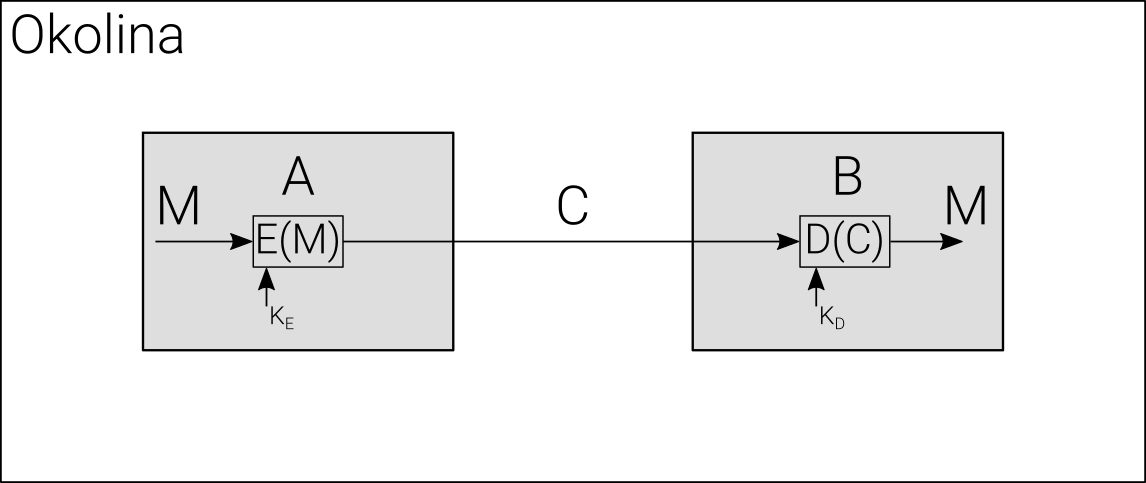
\includegraphics[width=12cm]{resources/images/SCA/traditional_model.png}
    \caption{Model tradicionalne kriptoanalize}
    \label{fig:traditional_model}
\end{figure}

\begin{figure}[htb]
    \centering
    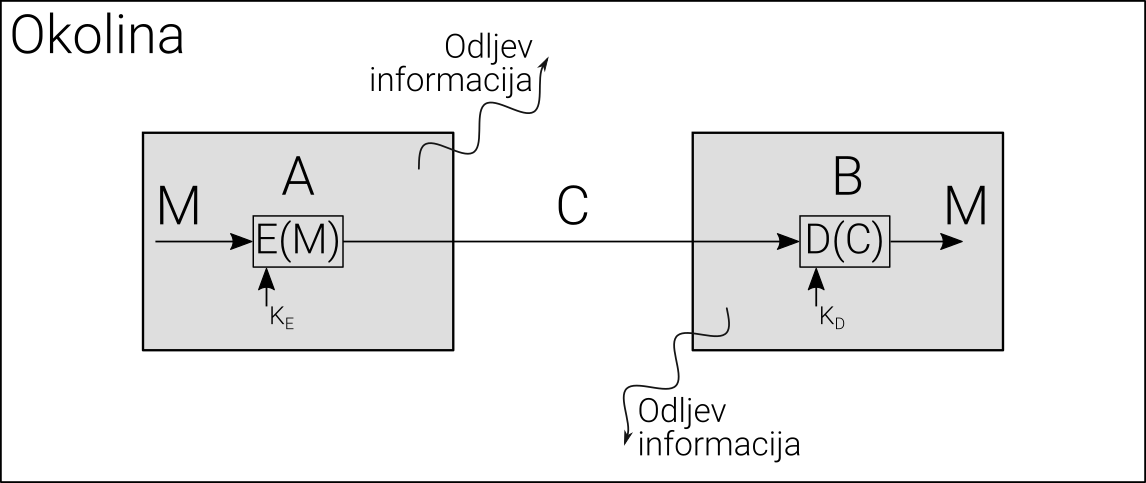
\includegraphics[width=12cm]{resources/images/SCA/SCA_model.png}
    \caption{Model SCA}
    \label{fig:SCA_model}
\end{figure}

Prema \cite{zhou2005side} jedna od najranijih instanci SCA napada se dogodila se još 1965. godine, kada je britanska tajna služba, MI6, pokušala probiti šifru koju je u to doba koristila egipatska ambasada, no slabi računalni resursi toga doba onemogućili su sve njihove pokušaje. Kako bi premostio taj problem, tadašnji GCHQ znanstvenik, P. Wright, predložio je da mikrofon bude postavljen blizu rotora kriptološkog uređaja korištenog od strane Egipćana i tako se omogućilo prisluškivanje zvukova kliktanja koje je uređaj proizvodio. Slušajući zvukove resetiranja rotora svako jutro britanska agencija je uspješno deducirala pozicije dva od tri rotora i time značajno smanjila računalne zahtjeve potrebne za dekripciju. MI6 je zbog ovog pothvata mogla prisluškivati komunikaciju ambasade godinama.

Moderne tehnike SCA su pionirane od strane Paula Kochera (\citeyear{kocher1996timing, kocher1999differential, kocher2004security}), koji je napisao da budući da na količinu električne energije uređaja utječu podaci koji se obrađuju, mjerenja potrošnje energije sadrže podatke o kalkulacijama kruga \citep{kocher2011introduction}. SCA metode napada pokazale su se znatno efektivnijima od konvencionalnih napada baziranih na matematičkoj analizi. Prilikom dizajniranja sigurnosnog sustava, dizajner na raspolaganju ima plato čvrstih formalnih metoda verifikacije kojima se u obzir uzimaju različiti tipovi napada pomoću kojih onda razmatra svojstva sigurnosti. Međutim, situacija je puno teža kada se odmaknemo od idealiziranih matematičkih modela do implementacije u stvarnom, fizičkom, svijetu. U ovakvoj situaciji postavlja se mnoštvo pitanja, poput koliki pristup uređaju će napadač imati, na koji način može manipulirati ulazima, kakve izlaze može identificirati i razaznati. No kao što smo rekli takvih izlaza ima puno, te ih je teško definirati. Kako bi se dizajnirao siguran sustav potrebno je puno iskustva, a za testiranje nije moguće koristiti formalne metode, već su potrebne simulacije i mjerenja na stvarnom uređaju nerijetko koristeći skupocjenu opremu. Zbog velike raznolikosti izvora informacija te nemogućnosti standardizacije, najteži dio dizajniranja sigurnog sustava je upravo detektiranje nedostataka. No "Historia est Magistra Vitae", povijest je učiteljica života, te je za bolje razumijevanje važno razumjeti postojeće napade koji će biti bolje objašnjeni u odjeljku \ref{sec:known_attacks}

\section{Osnove}

SCA napadi usko su vezani za postojanje fizički primjetnih fenomenima nastalim zbog izvođenja programa na današnjim mikrokontrolerskim uređajima. Na primjer mikroprocesori koriste električnu snagu i vrijeme kako bi izveli zadani zadatak, a pritom, zbog nesavršene efikasnosti uređaja emitiraju elektromagnetsko (skrać. \emph{EM}) zračenje jedno od kojih je toplina \citep{standaert2010introduction}. Iako postoji mnogo različitih izvora informacija koje se odlijevaju u okolinu, neke od kojih potencijalno još niti ne znamo, u ovom poglavlju, kako bi se ilustrirale tehnike SCA i dio pozadine od kuda one potiču, fokus će biti na dva tipa sporednih sredstava, a to su potrošnja energije i EM zračenje unutar CMOS tranzistora zbog njihove dominacije u svijetu integriranih krugova.


\subsection{Potrošnja energije CMOS uređaja} \label{sec:power_cmos}

Većina digitalnih uređaja zasniva se na CMOS vratima. To je sustav koji sa sastoji od dvije vrste tranzistora: pMOS tranzistora koji je spojen u načinu rada za pritezanje na napon napajanja \engl{pull-up} i nMOS tranzistora koji je spojen u načinu pritezanja na uzemljenje \engl{pull-down}. Tako je moguće izgraditi osnovne digitalne krugove, a zatim pomoću njih i kompleksnije sustave. Statička CMOS vrata imaju tri izrazita izvora disipacije. Prvi nastaje zbog unutarnjih struja samog tranzistora. Drugi izvor rezultat je činjenice da postoji kratak period prilikom promjene vrata kada i pMOS i nMOS tranzistori vode u isto vrijeme, zbog kojeg dolazi do takozvanih struja kratkog spoja \(I_d\) vidljivih na slici \ref{fig:short_circuit_current}.

\begin{figure}[htb]
    \centering
    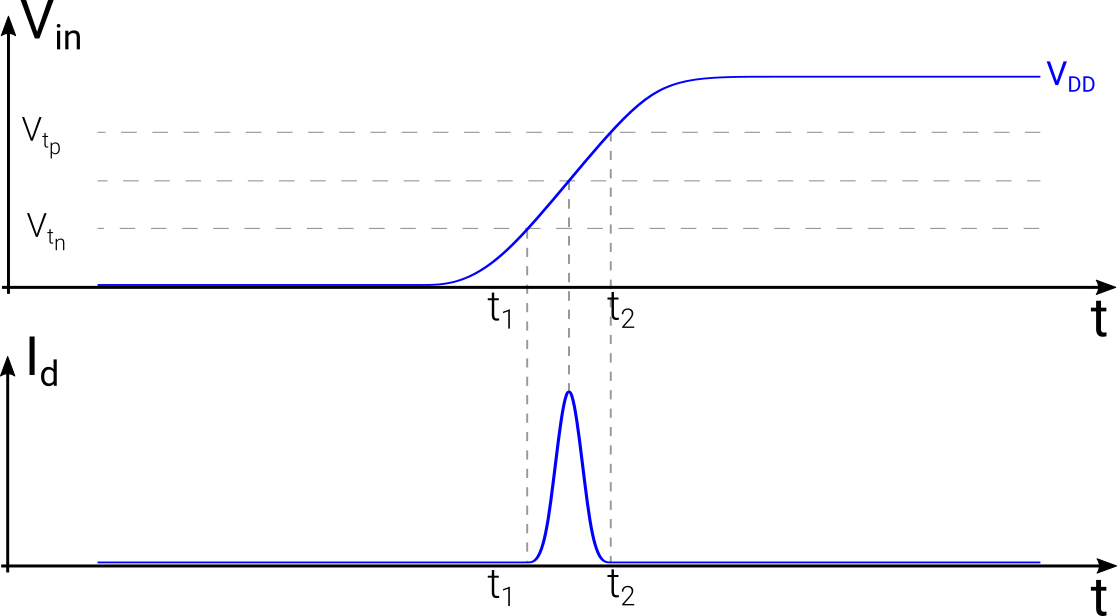
\includegraphics[width=12cm]{resources/images/SCA/short_circuit_current.png}
    \caption{Struja kratkog spoja prilikom promjene stanja}
    \label{fig:short_circuit_current}
\end{figure}

Treći razlog je zbog kapaciteta \(C_L\) tranzistora. Naime tranzistori imaju elektrode odvojene s tankim slojem dielektričnog materijala i time zapravo jesu fundamentalno i kondenzatori. Zbog toga postoji određena \emph{dinamička potrošnja energije} koja nastaje zbog punjenja i pražnjenja kondenzatora. Ona je posebno bitna u SCA jer je određena jednostavnom relacijom između unutarnjeg stanja uređaja i mjerljive fizikalne pojave. Taj odnos može biti izražena kao:
\begin{equation}
    P_d = C_L V_{DD}^2 P(0 \rightarrow 1) f
\end{equation}
gdje je \(P(0 \rightarrow 1)\) vjerojatnost da se dogodi promjena \(0 \rightarrow 1\), \(f\) radna frekvencija uređaja, a \(V_{DD}\) napon napajanja. Dakle kada mjerimo potrošnju energije šiljci će se pojavljivati prilikom pražnjenja i punjenja kondenzatora, točnije prilikom promjene stanja iz 1 u 0 ili obrnuto. Upravo ovakve povezanosti su izvor odljeva informacija.

\subsection{Elektromagnetsko zračenje CMOS uređaja}
Kao što je u prošlom odjeljku pokazan odnos između podataka i potrošnje energije, moguće je pokazati odnos između podataka i EM zračenja. Postoje dvije bitne povezanosti, prva je da je EM zračenje ovisno o jakosti struje koja je povezana s podacima, a druga orijentacija EM polja je ovisna o smjeru kretanja struje, za koju je također očito da je ovisna o podacima. Takvo EM zračenje često se teorijski modelira pomoću Biot-Savartovog zakona:
\begin{equation}
    dB = \frac{\mu I dl \times \hat{r}}{4 \pi r^2}
\end{equation}
Takvo zračenje također može biti opaženo mjerenjima te je neželjeni izvor informacija.

\subsection{Modeli odljeva}

Uzevši implementacijske detalje, poput onih opisanih u prošla dva poglavlja, razvijeni su brojni modeli odljeva koji se mogu koristiti za simuliranje napada ili povećavanje efikasnosti napada. Dva značajnija modela su model Hammingove udaljenosti i model Hammingove težine. Model Hammingove težine pretpostavlja da kada se računa vrijednost \(x_0\) tada je odljev u korelaciji s Hammingovom težinom te vrijednosti, \(H_W(x_0)\), dok model Hammingove udaljenosti pretpostavlja da kada u uređaju dođe do promjene iz vrijednosti \(x_0\) u vrijednost \(x_1\) tada vrijednost odljeva je u korelaciji s Hammingovom udaljenosti tih vrijednosti, tj. \(H_D(x_0, x_1) = H_W(x_0 \oplus x_1)\). Oba modela kao pretpostavku uzimaju da su događaji \(0 \rightarrow 1\) i \(1 \rightarrow 0\) utječu jednako na cjelokupnu potrošnju energije. Postoje kompleksniji modeli koji te pretpostavke umanjuju, primjerice koristeći različite odljeve za spomenute događaje ili dodjeljujući težinske vrijednosti doprinosima odljeva različitih dijelova sustava.

\subsection{Mjerenje}
Sa strane praktične implementacije SCA napada, dobro definirana mjerna shema je od primarne važnosti. Cilj je pretvoriti fizikalna svojstva ciljanog uređaja u digitalno iskoristive podatke. Elementi koji sačinjavaju takvu mjernu shemu generalno su:
\begin{itemize}
    \item ciljani uređaj, npr. integrirani ili FPGA krug koji izvodi neke kriptografske primitive, pametna kartica, itd.
    \item Vanjski izvor napajanja, generator pulsa i ostala električka oprema potrebna da uređaj radi ispravno.
    \item Sonda za mjerenje odljeva. Primjerice, otpornik male vrijednosti može se dodati u strujni krug napajanja te se tako može mjeriti potrošnja energije. Dodatno, EM zračenje može se mjeriti s jednostavnom ručno motanom zavojnicom.
    \item Uređaj za nadgledanje, npr. digitalni osciloskop s dovoljno velikom rezolucijom (tipično 1GS/s, 8 bitova rezolucije, ...) spojen na računalo za statističku analizu tragova.
\end{itemize}

Mjerne sheme imaju veliki utjecaj na efektivnost SCA napada. Pošto je šum glavni problem SCA napada, kvaliteta mjerenja se uglavnom kvantificira pomoću količine šuma u tragovima. Idealno, mjerenje bi trebalo biti izvedeno tako da sve njime dobivene informacije budu relevantne za analizu. Ovo naravno u praksi nije moguće.

\section{Klasifikacija napada} \label{sec:attacks}

SCA napadi uglavnom se klasificiraju u tri glavne skupine:

\begin{itemize}
    \item Klasifikacija prema kontroli nad procesom računanja
    \item Klasifikacija prema načinu pristupanja modulu
    \item Klasifikacija prema metodama korištenim prilikom analize
\end{itemize}

\subsection{Kontrole nad procesom računanja}

Prema različitim načinima kontrole napadača nad procesom izvođenja računa SCA napadi dijele se na dvije glavne kategorije: \textit{\textbf{pasivne}} i \textit{\textbf{aktivne}}. Ti napadi razlikuju se po interferenciji napadača na operativnost sustava. Kod pasivnih napada govorimo o napadu u kojemu napadač uspješno dohvati informacije o ciljanom sustavu ali operativnost tog sustava ostaje nepromijenjena, kakva bi i bila da se napad nije dogodio. Primjer takvog napada bilo bi prisluškivanje. Aktivni su napadi, s druge strane, oni kod kojih se direktno utječe na rad sustava. Ciljani sustav može ali ne mora moći detektirati da je došlo do napada, no vanjski promatrač može vidjeti promjenu u radu. Valja napomenuti da u ovakvom tipu napada nije zahtijevano da napadač dohvati informacije, već da samo ometa ciljani rad uređaja. Primjer ovakvog napada bila bi izmjena već poslane poruke.

\subsection{Načini pristupa modulu}

Prilikom analiziranja sigurnosti kripto procesora može biti korisno provesti sistematski presjek površine napada - skupa fizičkih, električkih i logičkih sučelja koji su izloženi potencijalnom napadaču. Vođeni ovom misli \cite{anderson2006cryptographic} podjeli su napade na sljedeće četiri skupine.

\paragraph{Invazivne napade \engl{Invasive attacks}}
To su oni napadi koji zahtijevaju direktan pristup unutarnjim komponentama kripto procesora. Na primjer napadač napravi rupu u unutrašnjost mikrokontrolera te direktno mjeri podatke s fizičke sabirnice. Iako je sondiranje dijelova mikročipa uvijek bilo dostupno proizvođačima poluvodičkih uređaja, sredinom 90-ih počela je pojava polovne opreme za testiranje poluvodiča na tržištima što je omogućilo invazivne napade široj populaciji. Tipična stanica za sondiranje sastoji se od mikroskopa montiranog na podlozi s minimalno vibracija. Mikroskop bi tipično sadržavao i laser s kojim bi se probijale rupe kroz pakiranje mikroprocesora. Proizvođači su razvili razne metode otpora na invazivne napade koje prilikom pokušaja napada trajno onesposobe uređaj. Također kako napredak tehnologije omogućuje da veličina komponenata korištenih u proizvodnji bude sve manja invazivni napadi postaju nepraktičniji i teži.

\paragraph{Polu-invazivne napade \engl{Semi-invasive attacks}}
Takvi napadi uključuju pristup uređaju ali bez potrebe za oštećenjem uređaja. Najraniji primjer ovakvog napada koristio je UV svijetlo kako bi se resetirao zaštitni biti na mikrokontroleru, kako bi se mogao pročitati sadržaj memorije. Još jedan od ranijih primjera bila je tehnologija testiranja poluvodiča prilikom koje je osvjetljavanjem nevodljivog CMOS transistora rezultiralo s mjerljivom strujom odljeva. No polu-invazivni napadi su postali praktični tek početkom 20-og stoljeća pojavom tehnika optičkog sondiranja. Ideja je da osvjetljavanjem transistora on postane provodljiv te da se tako uvede greška u njegovom radu. Takvi napadi mogu biti provedeni s jednostavnom opremom vrlo niske cijene. Korištenjem laserskih sondi, moguće je pasivno i čitanje memorijskog sadržaja ciljanog uređaja. To se postiže tako da se svaka memorijska ćelija osvijetli jedna po jedna, a rezultirana ionizacija prouzroči mjerljivu struju ako je sadržaj ćelije prazan.

\paragraph{Lokalno neinvazivne napade \engl{Local non-invasive attacks}} Ovakav tip napada uključuje promatranje ili manipulaciju rada uređaja koji se nalazi u neposrednoj blizini. Primjer ovakvog napada je mjerenje struje potrebne za rad procesa s visokom preciznošću te određivanje korelacije s trenutnim računanjem koje se izvodi kako bi se došlo do podataka, kao što je opisano u odjeljku \ref{sec:power_cmos}. Lokalno neinvazivni napadi spadaju u još generalniju skupinu napada, neinvazivne napade \engl{non-invasive attacks} zajedno s udaljenim napadima opisanim u sljedećem paragrafu. Bitna karakteristika neinvazivnih napada je da su potpuno neopazivi. Dodatno, ovakvi napadi uglavnom su jeftiniji od invazivnih napada, zbog čega predstavljaju veću prijetnju. Ovakav tip napada razmatrat će se u kasnijim poglavljima ovog rada.

\paragraph{Udaljene napade \engl{Remote attacks}} Prilikom napada ove vrste, rade se opservacije ili manipulacije normalnih ulaza i izlaza uređaja, a sam napad je neovisan o udaljenosti napadača od uređaja. Primjeri ovakvog napada uključuju vremensku analizu, kriptoanalizu i napade na aplikacijsko programsko sučelje. U ovu skupinu spadaju i tradicionalni kriptografski napadi koji iskorištavaju mane u kriptografskim primitivama i sigurnosnim protokolima. Kao što je već spomenuto ovakvi napadi također spadaju u neinvazivne napade.

\subsection{Metode korištene prilikom analize}

Prilikom podjele prema metodama korištenima prilikom analize podataka, SCA se dijeli na \textbf{jednostavnu} SCA (\englnp{Simple Side Channel Analysis}, dalje \emph{SSCA}) i \textbf{diferencijalnu} SCA (\englnp{Differential Side Channel Analysis}, dalje \emph{DSCA}).

SSCA karakterizira to da izlaz uglavnom ovisi o \emph{trenutnoj} operaciji koja se izvodi. Kod SSCA, tipično se koristi samo jedan trag \engl{trace} iz kojeg se tajni ključ može direktno odrediti. Zbog ovakvog pristupa SSCA je vrlo osjetljiv na šum, informacije iz sporednih sredstva koje nisu u korelaciji s podacima. Dakle bitno je da željeni signal, onaj povezan s traženim podacima bude izraženiji od šuma.

S druge strane, DSCA koristi korelaciju između procesiranih podataka i informacija sporednih sredstava. Kod DSCA generalno se koristi više tragova a zatim nad njima provodi statistička analiza kako bi se odredile informacije o ključu. DSCA se najčešće sastoji od sakupljanja informacija, a zatim njihove analize. Kako bi se efikasno analizirala korelacija podataka sa stvarnim, mjerljivim, informacijama koristi se hipotetski model uređaja koji je pod napadom. Taj model se koristi kako bi se predvidjela sporedna sredstva uređaja; to može biti samo jedan izvor informacija ili se može koristiti za modeliranje više različitih izvora. Ako se trag koristi samo jednom govorimo o \textbf{napadu prvog reda} \engl{first-order attack}, a ako se koristi dva ili više puta govorimo o \textbf{napadima drugog reda} \engl{second-order attack} i \textbf{napadima višeg reda} \engl{higher-order attack}, respektivno \citep{zhou2005side}.

\section{Postojeći napadi} \label{sec:known_attacks}

\subsection{Napadi analizom trajanja}

Napadi analizom trajanja \engl{timing attacks} su oni napadi koji se baziranu na tome da zbog optimizacija, kriptografski algoritmi uglavnom izvode operacije u ne konstantnom vremenu. Varijacije u trajanju izvođenja dakle mogu sadržavati informacije o operacijama koje su u tijeku. Ova ideju predstavio je \cite{kocher1996timing} a praktično je izvedena od \cite{dhem1998practical} koji su pokazali da je moguće osobnim računalom tadašnjice dekriptirati 512-bitni ključ u nekoliko sati s 300 000 mjerenja, te 128-bitni ključ s 10 000 mjerenja, čime su pokazali ozbiljnost ovakvih napada. \cite{brumley2005remote} su zatim pokazali da je, koristeći vremenske napade, moguće otkriti RSA privatne ključeve iz web servera baziranog na popularnom OpenSSL-u preko lokalne mreže. Pokazali su kako modificirana verzija Kocherovog napada može biti uspješno izvedena u ovakvom scenariju, tako što su napravili ~1/3 milijuna upita (~2 sata).

Jedna od jednostavnijih obrana je da parametri operacije ne budu ovisni o ulaznim podacima. Primjerice tako da sa slučajno generiranim podacima transformiramo parametre prije operacije a zatim poništimo obrnutom operacijom kasnije. Druga vrsta obrane je eliminacija grananja u računu kako bi trajanje bilo jednako za vrijednosti podataka. Iako ovakav način uspješno uklanja mogućnost ovakvog napada, on ujedno i donosi velike kazne u obliku vremena izvođenja. Noviji način rješavanja ovog problema je dizajniranje samog sklopovlja da sve operacije traju jednako, neovisno o tome koji podaci se obrađuju.


\subsection{Napadi greškom}

Pokazalo se da sklopovne greške i kvarovi nastali za vrijeme operacija kriptografskog sustava mogu dovesti do ozbiljnih sigurnosnih propusta. Ponašanje sustava za vrijeme stanja greške može pružiti uvid u njegov rad i dati informacije potrebne za uspješno dohvaćanje prividno sigurnih informacija. Napadi greškom \engl{fault attacks} predstavljaju praktične i efektivne napade protiv kriptografskih sklopovlja kao što su pametne kartice, a pomoću njih su gotovo svi kriptografski algoritmi probijeni. Napadi greškom jako variraju ovisno o ciljanom modulu, te mogućnostima napadača i tipu greške koja može biti izazvana.

Postoje dvije velike skupine sporednih sredstava omogućenih greškama. Prvi sredstvo je slanje namjerno iskvarenih podataka s ciljem da modul ne može uspješno rukovati takvim podacima. Drugo sredstvo je mogućnost stavljanja modula u ekstremne uvjete te tako uvesti grešku u njega. Neke od mogućih izvora smetnji mogu biti nagla promjena napona, temperature, svijetla, brzine pulsa...

Napadi greškom, predstavljeni prvi puta od \cite{boneh1997importance}, opisani su kao teoretski model napada na RSA potpise i Fiat-Shamir i Schnorr identifikacijske protokole.

Jedna od najjednostavnijih protumjera je, ako pretpostavimo da napadač ne može dva puta uvesti istu pogrešku, provesti neke operacije simetričnih algoritama dva puta, no to će naravno umanjiti performanse. Ili u slučaju javnih ključeve, dodatno provjeriti potpis s privatnim ključem neposredno prije slanja. Dodatno su predloženi drugi načini zaštite kao što su dodavanje kontrolne sume i randomizacija izvođenja.

\subsection{Napadi analizom snage}

Kao što je već opisano, potrošnja energije kriptografskih uređaja prilikom rada može dati dodatne informacije o operacijama koje se izvršavaju i uključenim podacima. Napadi koji iskorištavaju ovu činjenicu spadaju u skupinu napada analizom snage \engl{power analysis attacks}. Napadi ove vrste pokazali su se iznimno uspješnima za većinu tradicionalnih implementacija simetričnih i asimetričnih algoritama, te je u vrijeme pisanja ovog rada velika većina istraživanja u polju SCA upravo temeljena na njima. Polje analize snage dijeli se na \textbf{jednostavnu} analizu snage (\englnp{Simple Power Analysis, dalje \emph{SPA}}), \textbf{diferencijalnu} analizu snage (\englnp{Differential Power Analysis}, dalje \emph{DPA}) i \textbf{korelacijsku} analizu snage (\englnp{Correlation Power Analysis}, dalje \emph{CPA}).

U SPA napadima, cilj je pomoću analiziranja mjernih vrijednosti električne energije kroz vrijeme, odrediti koji uzorci vrijednosti predstavljaju koju instrukciju. Ideja je tako odrediti koja operacija se izvodi u koje vrijeme te koji su parametri te operacije. Primjerice, serija XOR operacija na osciloskopu izgleda drugačije nego serija operacija množenja. No kompleksni sustavi uglavnom izvode više operacija u isto vrijeme, zbog čega se stvara dodatni šum koji otežava SPA napade što nas dovodi do drugog tipa napada.

U DPA napadima, analiza snage provodi se i za vrijeme normalnih, kriptografskih operacija, te se ti podaci koriste kako bi se "oduzeli"
od onih dobivenih analizom snage za vrijeme izvođenja kriptografskih operacija. Na taj se način može umanjiti šum i poboljšati mogućnost uspješnog napad. Ovaj pristup, iako kompliciraniji, sličan je uklanjanju pozadinske buke iz zvuka. DPA i SPA napade razvili su \cite{kocher1999differential}, gdje su uspješno pokazali praktičan napad na implementacijsko sklopovlje DES algoritma.

Treća vrsta napada, su CPA napadi. Oni su statistički napadi koji koriste Pearsonov koeficijent korelacije. CPA je novija metoda te ima brojne prednosti naspram DPA, jedan od kojih je to da zahtjeva manji broj tragova potrebnih za uspješan napad. Ovu metodu prvi su opisali \cite{brier2004correlation}.

Neke od predloženih metoda obrane na razini sklopovlja jesu korištenje unutarnjeg izvora napajanja, randomiziranje redoslijeda izvođenja instrukcija, randomiziranje preimenovanja registara i korištenje dva kondenzatora, jedan koji se puni od vanjskog izvora i drugi koji pruža napajanje uređaju. S programske strane, jedna od predloženih mjera je uvođenje slučajnih instrukcija kako bi se promijenio uzorak potrošnje energije.

\subsubsection{Primjer DPA napada na DES algoritam}

Radi boljeg razumijevanja opisani su koraci izvođenja DPA napada na primjeru DES algoritma \citep{standaert2010introduction}:

\begin{enumerate}
    \item{\textbf{Odabir ciljanog algoritma i implementacije.}} Napadač prvo odredi algoritam (npr. DES) i ciljanu implementaciju (npr. ASCI ili FPGA) s koje namjera dohvatiti podatke.
    \item{\textbf{Odabir izvora odljeva i mjerne sheme.}} Napadač zatim odredi vrstu odljeva koji namjerava iskoristit (npr. potrošnja snage ili EM zračenje) i način na koji će mjerenjem pretvoriti taj odljev korisne podatke.
    \item{\textbf{Odabir ciljanog signala.}} SCA napadi uglavnom zasebno napadaju razne dijelove sustava, tj. tajnog ključa. Dakle, napadač bira koji dio ključa želi odrediti. Ovo može, na primjer, biti šest bitova ključa koji ulaze u prvu DES S-kutiju S0.
    \item{\textbf{Odabir ulaznih podataka.}} Ovisno o mogućnostima napadača, on može ili birati koji podaci ulaze u uređaj u obliku poruke ili ako to nije moguće pretpostavlja se da može nadzirati podatke koji ulaze.
    \item{\textbf{Određivanje unutarnjih vrijednosti algoritma.}} Za poznate ulazne poruke, napadač odredi vrijednosti ovisne o ključu unutar ciljanog uređaja koje se izračunavaju tijekom izvođenja algoritma. Iz računskih razloga, korisne su samo vrijednosti koje su ovisne o malom djelu ključa. Primjerice, moguće je predvidjeti prva četiri bita nakon permutacije u prvom krugu DES-a, za svaku od 64 moguće vrijednosti koje ulaze u S0. Kao rezultat ovoga napadač je predvidio unutarnje vrijednosti implementacije za $q$ poruka i za svaku razred mogućih ključeva $s^*$, koje sprema u vektore $\bm{v}_{s^*}^{(q)}$.
    \item{\textbf{Modeliranje odljeva.}} Za isti skup razreda mogućih ključeva dobivenih u prošlom koraku, napadač modelira funkciju stvarnog odljeva ciljnog uređaja. Primjerice, ako pretpostavimo da potrošnja CMOS uređaja ovisi o promjeni stanja, Hammingova težina ili udaljenost može biti korištena kako bi se predvidio odljev.
    \item{\textbf{Mjerenje odljeva.}} Mjerenjem stvarnog odljeva uređaja dobije se vektor odljeva $\bm{l_q} = \left[ l_1, l_2, \dots, l_q \right]$. On sadrži $q$ tragova koji odgovaraju $q$ različitih ulaza.
    \item{\textbf{Odabir relevantnih tragova.}} S obzirom na to da tragovi mogu sadržavati veliki broj uzoraka, generalno se oni filtriraju vizualno ili koristeći neke statističke metode. Kao rezultat ove faze dohvaćen je smanjeni vektor $R(\bm{l_q})$
    \item{\textbf{Statistička usporedba.}} Konačno, za svakog kandidata razreda ključeva, napadač radi statističku usporedbu predviđenog odljeva sa stvarnim mjerenim podacima. Ako je napad uspješan, očekivano je da model za odgovarajući ključi iz razreda daje najbolje rezultate usporedbe.
\end{enumerate}


\subsection{Napadi analizom EM zračenja}
Još jedan od opisanih sporednih sredstava je EM zračenje. Dakle uređaji zbog svoje operacije emitiraju EM polje, a kada se elektromagnetska zavojnica postavi u to polje, zbog Faradayevog zakona, u njoj će biti inducirana električna struja. Takva, mjerljiva, struja daje napadaču uvid u rad uređaja. Jedan od popularnijih napada ove vrste naziva se RFID skimming, a uključuje očitavanje RFID informacija s beskontaktne kartice prilikom korištenja. Uređaji potrebni za ovakav napad potpuno su legalni te se mogu kupiti u normalnim trgovinama električke opreme. Dodatno, većina modernih pametnih telefona ima NFC čitač koji se može koristiti u iste svrhe. Grana koja se bavi ovim napadima naziva se elektromagnetska analiza (\englnp{Electromagnetic Analysis}, dalje \emph{EMA}) te je po mnogim svojstvima slična analizi snage. Isto kao i analize snage, postoje dvije kategorije napada: \textbf{jednostavna} EMA (\englnp{Simple Electromagnetic Analysis}, dalje \emph{SEMA}) i \textbf{diferencijalna} EMA (\englnp{Differential Electromagnetic Analysis}, dalje \emph{DEMA}), a one se razlikuju na prijašnje opisane načine. Postojanje ovakvih sporednih kanala, u vojnim je krugovima, poznato već dulje vrijeme, vidljivo iz deklasificiranog dokumenta \citep{mcconnell1992national} američke nacionalne sigurnosne agencije \engl{National Security Agency, NSA} u kojem se raspravlja TEMPEST napad, daje se uputstvo instalacije opreme, te se istražuju razna komprimirana sredstva.

Protumjere protiv EM napada spadaju u dvije skupine, prva od kojih je smanjivanje jačine signala. Ovakva mjera uglavnom je na razini sklopovlja te uključuje redizajniranje uređaja i/ili stavljanje oklopa kako bi se umanjila količina EM zračenja vidljivog izvan modula. Druga skupina su metode smanjivanja količine informacije sadržane u signalu. To se postiže randomizacijom te čestim osvježavanjem ključa prilikom rada.

\subsection{Napadi koji koriste zvuk}

Zvuk je jedan od najranijih sporednih kanala, ali nedavno mu je ponovno pridodana pažnja kada su \cite{shamir2004acoustic} pokazali da postoji korelacija između zvuka proizvedenog od procesora i operacija koje se izvode. Ovakvi napadi uglavnom ne moraju brinuti o akustičnom šumu okoline, poput ventilatora od računala jer su ciljani zvukovi uglavnom frekvencija viših od 10Khz. A zbog razlika u sklopovlju, temperaturama i ostalim okolnim uvjetima, zvukovi različitih računalnih jedinica uglavnom imaju različite zvučne potpise. Dodatno, snimanjem pritisaka tipki može se odrediti unos s tipkovnice (uključujući tipkovnice bankomata) na temelju različitih zvukova koji svaka tipka proizvodi. Pomoću pravog mikrofona, zvuk ispisnih glava printeru može se upotrijebiti za rekonstrukciju ispisanog sadržaja. Uz to, nedavno je pokazano kako se samo snimanjem zvuka zavojnice \engl{coin whine} u radu LCD monitora može utvrditi što se na njemu prikazuje.
%\citep{gray-fow_2019}.

Neke od predloženih protumjera jesu korištenje opreme za prigušivanje zvuka, kao što su zvučno izolirane kutije dizajnirane specifično kako bi umanjile relevantne frekvencije. Suprotno tome, dovoljno jak širokopojasni izvor šuma može maskirati informativne signale, iako ergonomske zabrinutosti mogu ovakvu mjeru učiniti neprivlačnom.

\subsection{Napadi koji koriste vidljivu svjetlost}
\cite{kuhn2002optical} je demonstrirao da je moguće rekonstruirati sliku s CRT monitora ako taj monitor nije u vidokrugu napadača, već sve što je dostupno je difuzni odraz s primjerice obližnjeg zida. Pretpostavio je dodatno da se ista tehnika može iskoristiti i za druge izvore vidljive svjetlosti poput LED dioda. Kasnije su \cite{loughry2002information} pokazali kako postoji odnos između statusnih LED dioda računala i podataka koji se koriste u računu.

\subsection{Napadi koji koriste poruke o pogrešci}
U mnogim standardima, poput SSL/TLS, IPSEC, WTLS, poruke su prvo formatirane, a zatim enkriptirane ulančanim blokovskim šiframa (CBC). Na strani primatelja se za vrijeme dekripcije mora provjeriti valjanost formata. Informacija se lako odljeva iz komunikacijskih protokola u odabranom napadu, budući da primatelj uglavnom šalje potvrdu ili poruku o pogrešci. Ovo može postati korisno sporedno sredstvo za kriptoanalizu, a napadi koji ga koriste nazivaju se napadi koji koriste poruke o pogrešci \engl{Error message attack}. U praksi ovakva sredstva se pojavljuju jer napadač ima mogućnost da uvede predvidljive modifikacije u originalnoj poruci kroz modifikaciju kriptirane poruke. Ovakvi napadi pokazali su se uspješnima i kod simetričnih i asimetričnih kriptografskih algoritama. Najistaknutiji i uvjerljivi primjer napada koji koriste poruke o pogrešci vjerojatno je Bleichenbacherov (\citeyear{bleichenbacher1998chosen}) napad na RSA sustav. Zbog toga konsenzus je da je bitno uključiti snažnu provjeru integriteta u RSA enkripciju. Kod novijih inačica većine modernih algoritama, utjecaji ovakvog napada većinski su uklonjeni.

\subsection{Napadi bazirani na priručnoj memoriji}

Velika većina modernih procesora, uz primarnu i sekundarnu memoriju, implementira i treći tip memorije; priručnu memoriju \engl{cache}.
Ta memorija uglavnom je implementirana u samom procesoru te služi kao međuspremnik između procesora i radne memorije. Ona se koristi zbog činjenice da je brzina procesora puno veća od brzine radne memorije. Ako priručne memorije ne bi bilo procesor bi često morao čekati podatke iz radne memorije, a ta bi komunikacija postala usko grlo \engl{bottleneck} sustava. No uz korištenje priručne memorije podaci za koje se očekuje pristup spremaju se u priručnu memoriju i tako se znatno smanjuje vrijeme čekanja podataka i ubrzava rad sustava. Ako procesor zatraži podatak koji se nalazi u priručnoj memoriji, to nazivamo pogodtkom \engl{cache hit}, a ako to nije slučaj to nazivamo promašajem \engl{cache miss}. Promašaji pričuvne memorije iznimno su bitan pojam u polju programske optimizacije, ali pokazalo se da mogu biti vrlo bitni i u polju SCA. Naime, ako se dogodi promašaj, generirat će se kašnjenje u izvođenju zbog navedenih razloga. Mjerenje trajanja tog kašnjenja napadaču omogućuje da sazna kada se promašaj dogodio te frekvenciju pojavljivanja istih. Upravo to je ideja napada baziranih na priručnoj memoriji \engl{Cache-based attacks}. Originalna ideja ovakvog napada je predložena od strane \cite{kelsey1998side}. Napadi "Spectre" i "Meltdown" spomenuti u uvodu, jedni su modernijih napada koji koriste slabosti nastale zbog priručne memorije.

Razne mjere obrane su predložene, poput uklanjana priručne memorije, ali efikasno rješenje koje ne ovisi o izvedbi je još uvijek otvoreno pitanje.

\subsection{Napadi bazirani na frekvenciji}

Ovu relativno noviju ideju, predložio je \cite{tiu2005new}. Metoda je efektivna čak i kad tragovi nisu poravnati u eksperimentu, uvjet koji nije bio ispunjen dotadašnjim DEMA istraživanjima. Glavne mete ovakvog napada su prijenosni uređaj, poput mobitela i digitalnih osobnih asistenata. Dodatno, za predloženu diferencijalnu frekvencijsku analizu (\englnp{Differential Frequency Analysis}, dalje \emph{DFA}) prvog reda, pokazano je da je uspješna usprkos dodavanju slučajnog kašnjenja. No ova je metoda neuspješna kada se u AES protokol implementira protumjera razdijeljenom maskom \engl{Split Mask}.

\subsection{Napadi bazirani na skeniranju}

Kako su logički uređaji postajali sve kompleksniji, zahtijevalo se puno više vremena i truda potrebnog za ručno stvaranje i validiranje testova. Također je bilo sve teže odrediti koji postotak funkcionalnosti test pokriva, a sami testovi trajali su predugo. Ovako opisana tehnika testiranja naziva se funkcijsko testiranje. No zbog nepraktičnosti, industrija je krenula s takozvanim "dizajniranje za testiranje" \engl{design to test, DFT} pristupom, gdje je sam dizajn modificiran kako bi bilo jednostavnije testirati sklopovlje. De facto standard ovakvog testiranja je test "skeniranjem" \engl{scan test}. Bistabili sadržani u dizajnu modificirani su kako bi im se omogućilo da za vrijeme testiranja funkcioniraju kao stimulans i točke na kojima se mogu validirati ispravnosti, a da i dalje za vrijeme normalne operacije izvršavaju svoju standardnu ulogu.

\begin{figure}[htb]
    \centering
    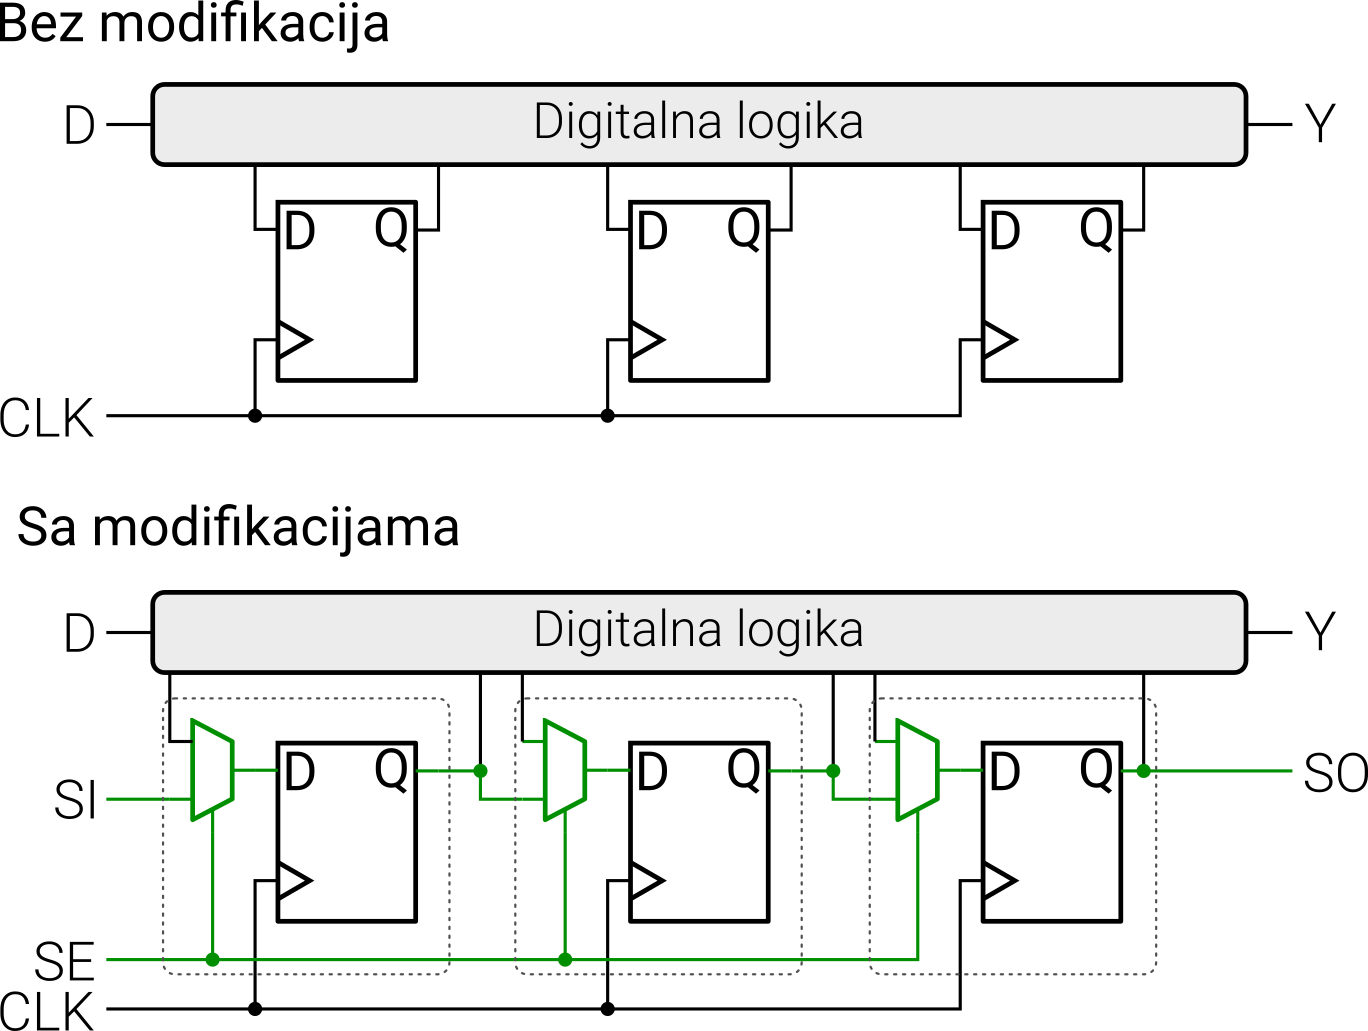
\includegraphics[width=11cm]{resources/images/SCA/scan-test.png}
    \caption{Ne modificirani i modificiran dizajn}
    \label{fig:scan-test}
\end{figure}

Budući da test skeniranjem mijenja bistabile koji su već uključeni u dizajn kako bi omogućio da djeluju i kao stanice za skeniranje, utjecaj testnog kruga je relativno mali, obično dodaje samo oko 1-5\% na ukupan broj vrata. \citep{semiconductorengineering_2019}
Očito je da su testovi skeniranja bitni za razvoj digitalnih uređaja, no isto tako \cite{yang2004scan} pokazali su da je i korisno sporedno sredstvo u tzv. napadima baziranim na skeniranju \engl{scan-based attacks}, tako što su iskorišteni već postojeći skenirajući lanci za dobivanje tajnog ključa iz sklopovske implementacije DES algoritma. Naravno s pažljivim dizajniranjem i odspajanjem lanaca nakon testiranja ovakve je napade moguće izbjeći.

\section{Protumjere}

Kako su se napadi razvijali, tako su i razvijale protumjere za njih. Postoji mnogo raznih strategija obrane od napada koji koriste sporedna sredstva, neke generalne jesu:
\begin{itemize}
    \item ukloniti korelaciju između izlaznih tragova (npr. pomoću dodavanja slučajnih vremenskih pomaka, umetanja lažnih instrukcija, randomizacijom redoslijeda izvođenja, itd..);
    \item zamijeniti kritičke instrukcije s onima čiji "potpis" nije jednostavno analizirati ili redizajnirati sklopovske komponente koje izvode aritmetičke operacije i/ili prebacivanje podataka iz memorije;
    \item napraviti algoritamske promjene kriptografskih primitiva kako bi napadi bili neučinkoviti na dobivenoj implementaciji (npr. maskiranje podataka i ključa sa slučajnom maskom generiranom pri svakom pokretanju)
\end{itemize}

Pokazano je da su algoritamske tehnike među svim tim vrstama protumjera najsvestranije, sve prožimajuće i mogu biti najefikasnije. Također, u mnogim su kontekstima one najjeftinije za provedbu. Programske mjere uključuju uvođenje lažnih instrukcija, randomizacijom redoslijeda izvođenja, uravnoteživanje Hammingove težine unutarnjih podataka i dijeljenje bitova. Na razini sklopovlja, protumjere obično uključuju randomizaciju takta, randomizaciju ili kompenzaciju potrošnje energije, randomizaciju izvršavanja instrukcijskog skupa i/ili korištenja registara. Ovakve mjere uglavnom su mnogo skuplje za provedbu, a njihov se učinak može umanjiti raznim tehnikama obrade signala. Dok programske mjere protiv SCA napada znatno ometaju izvedbu kriptografskih algoritama u pogledu memorije ili vremena izvođenja ili oboje. Jedan od glavnih izazova je postići sigurnu implementaciju sa što manje dodatnih troškova.

Odabir odgovarajuće razine protumjera može ovisiti o vrijednosti ciljanih podataka i moći protivnika (na primjer, njegovom znanju, resursima, itd.). Procjenjivanje razine otpora treba obaviti barem iz sljedeća tri ugla: moć protivnika (uključujući njegovo znanje, resurse i vještine i dr.), moć napada (koja je usko povezana s najsuvremenijom tehnologijom) i djelotvornost protumjera. Do sada se pokazalo da kombinacija sklopovskih i algoritamskih mjera zaštite daje vrlo dobar omjer sigurnosti i troškova. \citep{zhou2005side}.

\subsection{Randomizacija}

U SCA napadima, napadač pokušava povezati uzorke inherentne sporednim svojstvima s operacijama i podacima koji se obrađuju. Kako bi se to otežalo, jedna metoda je randomizirati podatke koji istjecaju kroz razne sporedna sredstva, kao što su potrošnja energije, EM zračenje ili duljina trajanja izvršavanja. Ideja je tako, sa strane napadača, smanjiti korelaciju, te tako i mogućnost dobivanja korisnog znanja o unutarnjem radu sustava.
U slučaju kriptosustava koji koriste eliptične krivulje, metoda randomiziranih projektivnih koordinata je praktična protumjera protiv napada SCA u kojima napadač ne može predvidjeti pojavu određene vrijednosti jer su koordinate slučajno generirane. U ovakvom slučaju standardni DPA koristi korelacijsku funkciju koja može razlikovati je li određeno sredstvo povezano s opaženom operacijom. Kako bismo to izbjegli potrebno randomizirati i parametre eliptičkih krivulja.

\subsection{Zasljepljivanje}

Zasljepljivanje je koncept u kriptografiji koji omogućuje klijentu, da postoji poslužitelj koji računa matematičku funkciju \(y = f(x)\), gdje klijent pruža ulaz \(x\) i dohvaća odgovarajući izlaz \(y\), ali poslužitelj ne bi saznao ništa o \(x\) ni \(y\). Ovaj koncept koristan je kada klijent ne može računati matematičku funkciju \(f\) sam \citep{Bleumer2011}.

Kao primjer, sagledajmo sljedeću situaciju: klijent želi dekriptirati podatak \(x\), tj. želi odrediti \(y \equiv x^d \pmod{n}\), uz ulaz \(x\). Kako poslužitelj ne bi mogao znati ni \(x\) a ni \(y\) moramo iskoristiti tehnike zasljepljivanja; klijent odabere slučajan broj \(r\) a zatim odredi \(s \equiv r^e \pmod{n} \). Tada je podatak koji šalje poslužitelju \( X \equiv xs \pmod{n}\). Poslužitelj zatim računa \(Y \equiv X^d \pmod{n}\), a izlaz \(Y\) zatim dohvaća klijent, koji ga pretvara u \(y \equiv \frac{Y}{r} \pmod{n}\). Vidljivo je da vrijedi
\begin{equation}
    y \equiv
    \frac{Y}{r} \equiv
    \frac{X^d}{r} \equiv
    \frac{(xs)^d}{r} \equiv
    \frac{x^d s^d}{r} \equiv
    \frac{x^d r}{r} \equiv
    x^d \pmod{n},
\end{equation}
što je upravo ono što smo htjeli izračunati, ali poslužitelj je znao samo vrijednost \(X\) i \(Y\), bez poznavanja \(x\) i \(y\).

Tehnike zasljepljivanja su najefektivnija mjera obrane napada analizom potrošnje energije i napada koji koriste trajanje.

\subsection{Maskiranje}

Maskiranje podataka je proces sakrivanja originalnih podataka pomoću modificiranog sadržaja. Ta tehnika je najrasprostranjenija protumjera protiv  napada analizom potrošnje energije i napada koji koriste trajanje na programskoj razini. Ona je također jedna od najboljih programskih protumjera protiv SCA napada. Maskiranje podataka zasniva se na jednostavnoj ideji, da se poruka i ključ maskiraju sa slučajno generiranom maskom na početku izračuna, nakon čega se ostatak izvodi jednako kao i bez maske. Naravno, na kraju je potrebno da maska bude poznata kako bi se podaci mogli obnoviti. Taj proces naziva se korekcija maske, \engl{mask correction}.

\chapter{Smanjenje dimenzionalnosti}

Smanjenje dimenzionalnosti \engl{dimensionality reduction} je jednostavno rečeno proces smanjivanja dimenzija skupa značajki.

Kada pričamo o podacima iz stvarnog svijeta, skup podataka uglavnom je sastavljen od velikog broja značajki. Redukcijom dimenzionalnosti pomažemo ukloniti nepotrebne značajke, smanjujemo računalne zahtjeve (vremenske i prostorne) i uklanjamo šum. Time omogućavamo bolju generalizaciju te smanjujemo mogućnost prenaučavanja \engl{overfitting}.

\paragraph{Hughesov fenomen}
pokazuje da kako broj značajki raste, raste i učinak klasifikatora sve dok ne dosegnemo optimalni broj značajki. Dodavanje više značajki će dalje smanjivati učinak, vidljivo na slici \ref{fig:hughes}. Ovaj fenomen prvi je objavio i detaljno objasnio \cite{hughes1968mean} te je po njemu dobio ime. Intuitivno objašnjene je da kako bi istrenirali dobar sustav za predviđanje on mora "vidjeti" puno mogućih kombinacija vrijednosti kako bi naučio uzorke u podacima. S više značajki postoji puno više kombinacija tako da je potrebno i puno više primjera. Hughes je također pokazao da ukoliko bi imali beskonačan izvor primjera rast dimenzija bi kontinuirano rezultirao i rastom točnosti klasifikatora, no to naravno nije moguće u stvarnom svijetu.
\begin{figure}[htb]
    \centering
    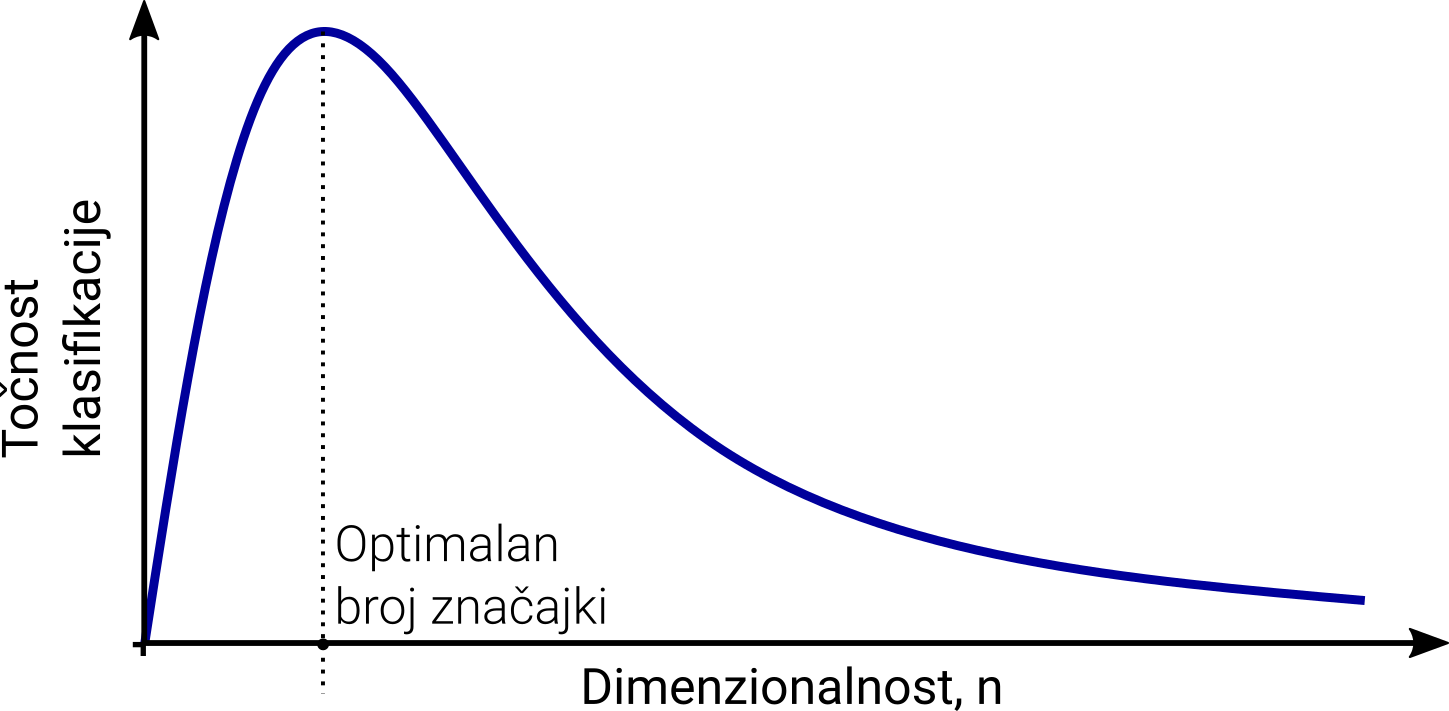
\includegraphics[width=12cm]{resources/images/reduction/hughes.png}
    \caption{Odnos dimenzionalnosti i točnosti klasifikacije}
    \label{fig:hughes}
\end{figure}

Ovo je ujedno i oblik prokletstva dimenzionalnosti. Dakle kako naša dimenzionalnost raste u jednom trenutku sposobnost generalizacije klasifikatora pada.

\bigskip
Redukcija dimenzionalnosti može se napraviti na razne načine. Najosnovniji od kojih je odabir značajki \engl{feature selection}. Odabir se može izvoditi ili ručno ili algoritamski. Jedan od popularnijih primjera je postavljanje praga na varijancu \engl{variance threshold}. Dakle ako značajka ima jako malu varijancu kroz primjere sigurno je pretpostaviti da neće mnogo pridonijeti predviđanju.

\medskip
Osim odabirom značajki redukcija se može raditi transformacijom prostora, koja može biti linearna ili nelinearna. Ako se radi o linearnoj transformaciji, govorimo o linearnoj redukciji dimenzionalnosti, neke od čijih metoda su PCA, analiza faktora \engl{Factor analysis} i LDA. Jednako, ako je riječ o nelinearnoj transformaciji prostora tada pričamo o nelinearnoj redukciji dimenzionalnosti. Nelinearna redukcija dimenzionalnosti često se naziva i učenje mnogostrukosti. Ove dvije metode bit će objašnjene u odjeljcima \ref{sec:lin_reduc} i \ref{sec:nonlin_reduc} respektivno.

\medskip
Još jedna vrlo zanimljiva metoda redukcije dimenzionalnosti koja daje izvanredne rezultate su autoenkoderi. Auto enkoderi se u svojoj suštini sastoje od dvije neuronske mreže, prva, koja se naziva enkoder, uzima originalni ulaz \(x \in \mathbb{R}^n\) te ga smanjuje u takozvanu latentnu reprezentaciju \(h \in \mathbb{R}^m\), gdje je \(m < n\). Druga mreža, pod imenom dekoder, pretvara izlaz prvog u idealno kopiju originalnog ulaza \(x' \approx x\). Ovaj proces vidljiv je na slici \ref{fig:autoencoder}.

\begin{figure}[htb]
    \centering
    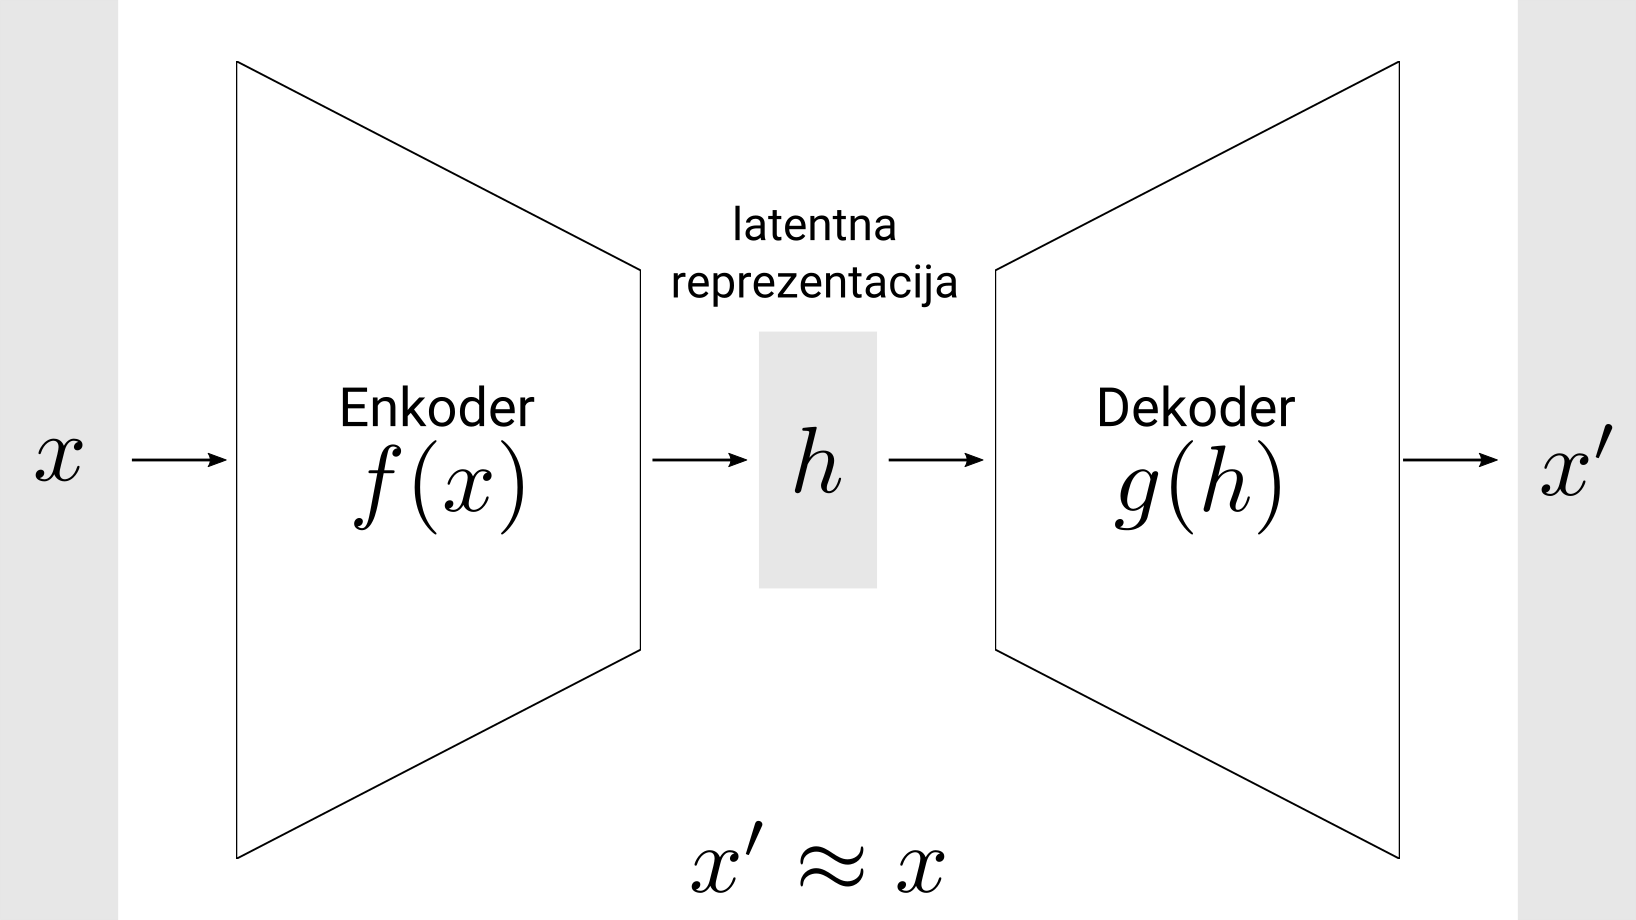
\includegraphics[width=12cm]{resources/images/reduction/autoencoder.png}
    \caption{Autoenkoder}
    \label{fig:autoencoder}
\end{figure}

\section{Linearna redukcija dimenzionalnost}\label{sec:lin_reduc}

Linearna redukcija dimenzionalnosti \engl{linear dimensionality reduction} je najraširenija metoda redukcije dimenzionalnosti. Moguće ju je vidjeti u poljima poput statistike analize, strojnog učenja i primijenjenim područjima matematike kroz stoljeća. Postala je neophodan alat za analiziranje visokodimenzionalnih, podataka s mnogo šuma. Ovakve metode stvaraju niskodimenzionalno linearno mapiranje originalnih visokodimenzionalnih podataka, ali tako da zadrže željene značajke.

\begin{definition}[Linearna transformacija]
    Neka $V$ i $W$ budu vektorski prostori na istom polju $K$. Tada za funkciju $f: V \mapsto W$ kažemo da je linearna transformacija (mapiranje) ako uz $\forall u,v \in V$ i $\forall c \in K$, vrijede sljedeća svojstva:
    \begin{center}
        \begin{varwidth}{\textwidth}
            \begin{enumerate}
                \item $f(u + v) = f(u) + f(v)$
                \item $f(cu) = cf(u)$
            \end{enumerate}
        \end{varwidth}
    \end{center}
\end{definition}
Dakle može se reći da je linearna transformacija ona koja očuva operacija zbrajanja i množenja.

Postoje mnogo raznih metoda linearne redukcije dimenzionalnosti samo neke od kojih su analize glavnih komponenata \engl{Principal Component Analysis, PCA}, analiza faktora \engl{Factor Analysis, FA}, linearna diskriminantna analiza, \engl{Linear Discriminant Analysis, LDA}, kanonička korelacijska analiza \engl{Canonical Correlations Analysis, CCA} i mnoge druge. Za potrebe ovog rada bit će obrađena PCA analiza, ali pregled i uvid u druge metode linearne analize moguće je vidjeti u \cite{cunningham2015linear}.

\subsection{Analiza glavnih komponenti - PCA}

PCA je daleko jedna od najpopularnijih metoda redukcije dimenzionalnosti, prvi put prezentirana od Karla Pearsona (\citeyear{pearson1901liii}) kao minimizacija kvadratnog zbroja rezidualne pogreške između originalnih i projiciranih podataka. Moderne inačice PCA uglavnom rade ekvivalentnu maksimizaciju variance. Statistički, PCA traži linije, ravnine i hiper-ravnine u n-dimenzionalnom prostoru tako da koordinate imaju najveću moguću varijancu podataka. Primjer je vidljiv na slici \ref{fig:pca}. Prva glavna komponenta ($pc_1$) je linija koja predstavlja smjer najveće varijance podataka. Za drugu komponentu ($pc_2$) vrijedi da je ortogonalna na prvu, da prolazi kroz centroid, a da pokazuje smjer drugog najvećeg smjera varijance. Jednako tako opisuju se i sve sljedeće komponente.
\begin{figure}[htb]
    \centering
    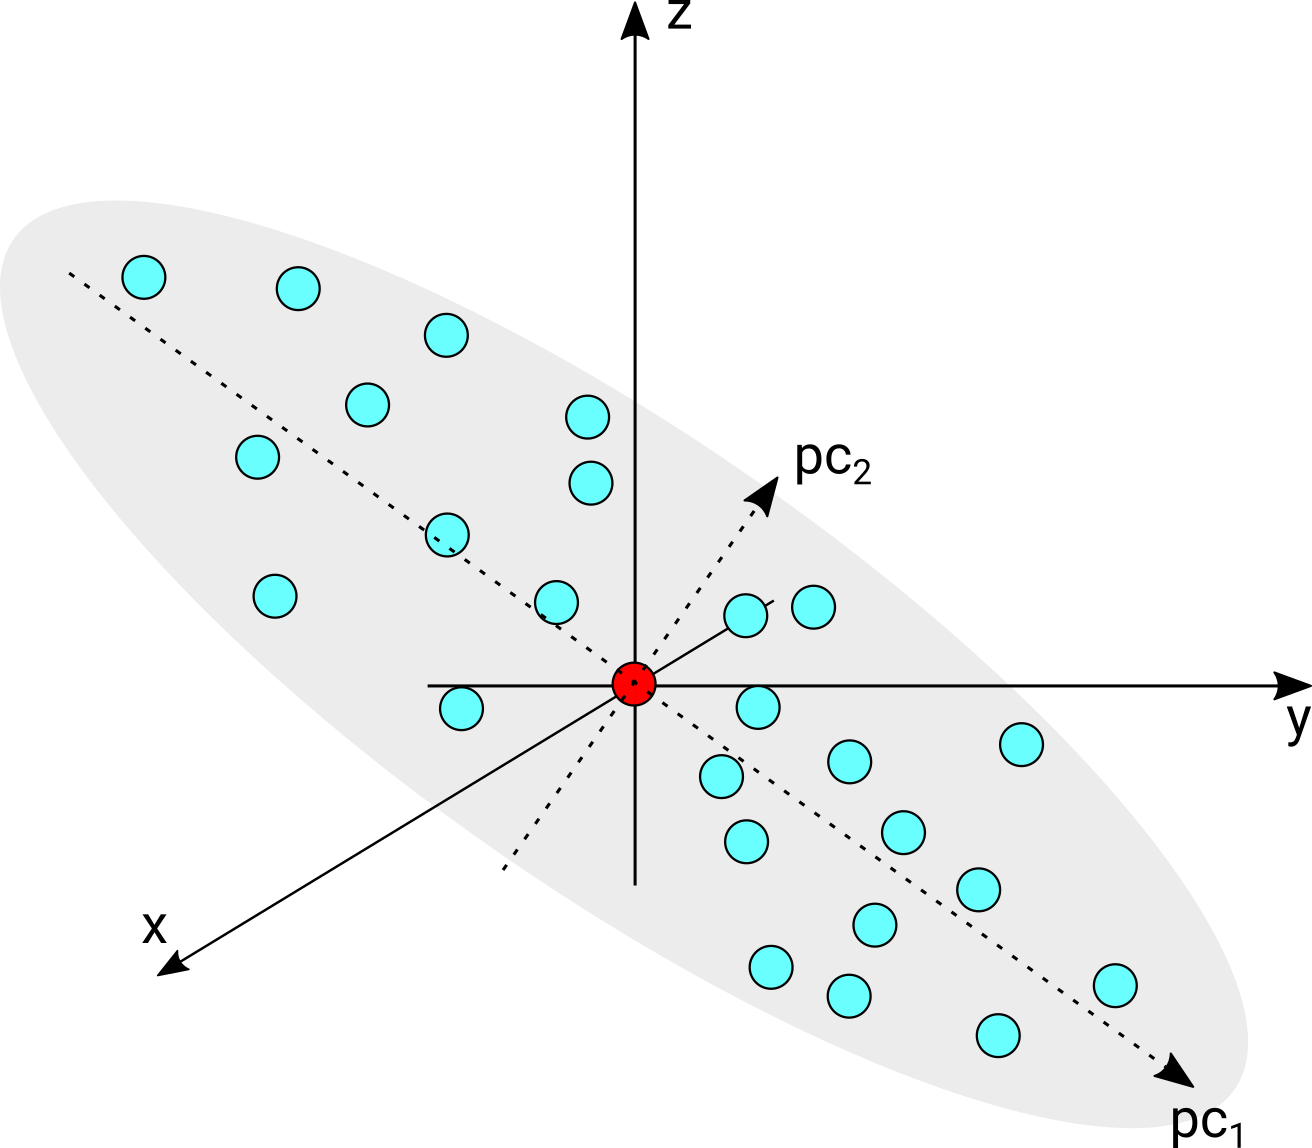
\includegraphics{resources/images/reduction/pca.png}
    \caption{Primjer PCA}
    \label{fig:pca}
\end{figure}

PCA se sastoji od nekoliko koraka.
Prvi korak je standardizacija. Podaci se transformiraju kako bi imali srednju vrijednost $\mu$ jednaku 0 i standardnu devijaciju $\sigma$ jednaku 1 prema jednadžbi \ref{eq:standardization} za svaki \(x\).
\begin{equation}
    z = \frac{x - \mu}{\sigma}
    \label{eq:standardization}
\end{equation}
Time efektivno centroid naših podataka pomičemo u ishodište koordinatnog sustava. Na slici \ref{fig:pca} ovaj korak je već izveden te je centroid označen crvenom bojom.

Sljedeći korak je odrediti glavne komponente. Kako bismo to odredili potrebno je prvo izračunati kovarijancijsku matricu koristeći formulu \ref{eq:covar}.
\begin{equation}
    cov(X, Y) = \frac{1}{i - 1}\sum_{n=1}^{n} (X_i - \bar{x})(Y_i - \bar{y})
    \label{eq:covar}
\end{equation}
Cilj ovog koraka je razumjeti kako se varijable skupa ulaznih podataka razlikuju od srednje vrijednosti u odnosu jedna na drugu ili drugim riječima kako bi se utvrdilo postoji li međusobna veza. Valja naglasiti da zbog činjenice da je $cov(x, x) = var(x)$, na glavnoj dijagonali kovarijancijske matrice nalaze se varijance originalnih značajki, a zbog toga što je operacija računanja kovarijance komutativna tj. vrijedi $cov(x,y) = cov(y, x)$, matrica je simetrična u odnosu na glavnu dijagonalu.

Nakon što znamo kovarijancijsku matricu, potrebno je izračunati njene vlastite vektore \engl{eigenvectors} i vlastite vrijednosti \engl{eigenvalues} kako bismo odredili glavne komponente.

\begin{definition}
    Za danu kvadratnu matricu $A \in \mathbb{R}^{n \times n}$, ponekad je moguće pronaći ne-nul vektor $v \in \mathbb{R}^n$ i odgovarajući skalar $\lambda$ takav da vrijedi
    \begin{equation}
        Av = \lambda v.
        \label{eq:eigen}
    \end{equation}
    Tada za svaki ne-nul vektor $v$ koji zadovoljava \ref{eq:eigen} zovemo vlastiti vektor od $A$, a odgovarajući skalar $\lambda$ vlastitu vrijednost.
\end{definition}
Očito je da jednadžba \ref{eq:eigen} može biti zapisana i kao
\begin{equation}
    (A - \lambda I)v = 0.
\end{equation}

Glavne komponente su nove varijable koje se grade kao linearne kombinacije početnih varijabli. Te se kombinacije izvode na takav način da su nove varijable (tj. glavne komponente) nekorelirane, a većina informacija unutar početnih varijabli se komprimira u prve komponente. Dakle ideja je da n-dimenzionalni podaci rezultiraju s n glavnih komponenti, ali se maksimalno moguće informacija "stavlja" u prvu komponentu, za zatim maksimalno preostalih informacija u drugu i tako dalje. Tako može se uzeti nekoliko prvih dimenzija, a ne izgubiti mnogo informacija. To je moguće jednostavno odrediti koristeći izračune vlastite vektore i pripadne vlastite vrijednosti, tako da se "uzmu" vlastiti vektori koji imaju najveću pripadnu vlastitu vrijednost i od njih napravi takozvani vektor značajki \engl{feature vector}. Dakle vektor značajki je jednostavno rečeno matrica koja kao stupce sadrži, po pripadnoj vlastitoj vrijednosti poredane, vlastite vektore koji su odlučeni biti zadržani. Dakle ako je cilj da konačna dimenzija prostora bude $m$ tada će ta matrica imati $m$ stupaca.

Osim standardnog PCA postoje i druge inačice kao što su iterativni PCA i nelinearni PCA koji koristi razne jezgrene \engl{kernel} funkcije.

\newpage
\section{Nelinearna redukcija dimenzionalnost}\label{sec:nonlin_reduc}

Nelinearna redukcija dimenzionalnosti u literaturi često se naziva i učenje mnogostrukosti \engl{manifold learning}. Za razumijevanje potrebno je prvo objasniti mnogostrukost.

\paragraph{Mnogostrukost}
U matematici, n-dimenzionalna topološka mnogostrukost ili samo mnogostrukost je apstraktni topološki prostor koji je lokalno euklidski, tj. za koji vrijedi da oko svake točke postoji susjedstvo koje je topološki jednako kao otvorena jedinična kugla u n-dimenzionalnom prostoru $\mathbb{R}^n$. Za ilustraciju ove ideje, dovoljno je sagledati vjerovanja da je Zemlja ravna ploča u kontrastu modernih dokaza da je okrugla. Ta nedosljednost uglavnom proizlazi iz činjenice da na malim mjerilima kojima ljudi vide Zemlju ona doista izgleda ravno. Generalno, svi objekti koji su približno "ravni" na malim mjerama su mnogostrukosti \citep{rowland}.
Za potrebe ovog rada, iako ne potpuno ispravno, dovoljno je gledati na mnogostrukost kao generalizaciju jednostavne n-dimenzionalne površine.

\paragraph{Hipoteza o mnogostrukosti} jedna je od najvažnijih hipoteza cijelom strojnom učenju. Ona kaže da podaci iz stvarnog života, poput slika, leže na niskodimenzionalnoj mnogostrukosti ugrađenoj u visokodimenzionalni prostor. Intuicija kaže da bi ona trebala vrijediti jer slični podaci će u prostoru biti relativno blizu. Ako za primjer uzmemo kameru koja može rotirati oko dvije osi, tj. ima dva stupnja slobode, te tako iz više položaja slika objekt. Recimo da kamera uzima slike rezolucije 640x480, tada će svaka naša slika imati 307200 značajki, točnije ležat će u 307200-dimenzionalnom prostoru. No znamo da te slike ovise o položaju naše kamere koji je moguće opisati samo s dvije značajke (rotacijom oko svake od osi), te imamo razloga vjerovati da naše slike leže na dvodimenzionalnoj mnogostrukosti koja je ugrađena u taj 307200-dimenzionalni prostor.

\paragraph{Učenje mnogostrukosti} leži na hipotezi o mnogostrukosti. To je skupni naziv za metode pronalaženja niskodimenzionalne mnogostrukosti ugrađene u visokodimenzionalni prostor za koji hipoteza o mnogostrukosti tvrdi da postoji.

\section{Algoritmi za učenje mnogostrukosti}

Postoji mnogo algoritama za učenje mnogostrukosti, no ovdje ćemo navesti samo one implementirane u poznatoj knjižnici jezika python – scikit-learn. Dodatno razmatrat će se i relativno novija metoda UMAP implementirana u umap-learn python knjižnici.

\subsection{Multidimenzionalno skaliranje - MDS}

Multidimenzionalno skaliranje (\englnp{Multidimensional scaling}, skrać. \emph{MDS}) grupni je naziv za skup metoda koje predstavljaju mjere sličnosti između parova objekata kao udaljenost između točaka u niskodimenzionalnom prostoru. Podaci, na primjer, mogu biti korelacija između objekata, tada je MDS reprezentacija ravnina koja prikazuje točke koje su bliže jedno drugoj što je njihova korelacija veća. U općem slučaju MDS može se koristiti za analiziranje sličnosti i različitosti u podacima, tako što sličnost ili različitost modelira kao udaljenosti u geometrijskom prostoru \citep{borg2005modern}.

\begin{figure}[htb]
    \centering
    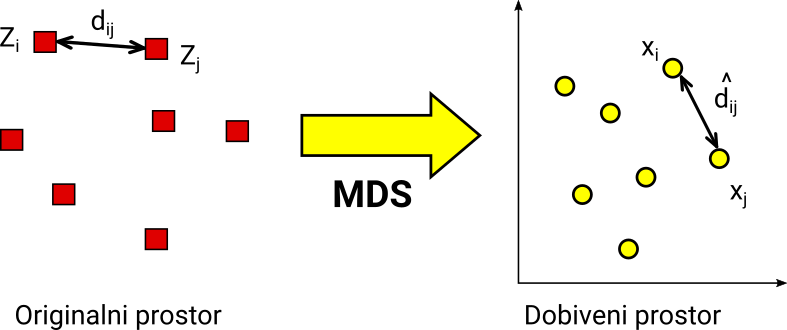
\includegraphics[width=12cm]{resources/images/reduction/mds_mapping.png}
    \caption{Prikaz preslikavanja MDS-a}
    \label{fig:mds_mapping}
\end{figure}

\begin{definition}
    Neka je matrica $S$ matrica sličnosti, a $X$ koordinate od $n$ ulaznih točaka. Također neka su razlike $\hat{d}_{ij}$ transformacija od $S$ odabrana na neki optimalan način. Tada definiramo mjeru $Stress$ kao:
    \begin{equation}
        Stress_r(X) = \sum_{i < j} (d_{ij}(x) - \hat{d}_{ij}(X))^2
    \end{equation}
\end{definition}
Ova mjera je ujedno i željena funkcija gubitka koja se minimizira. $Stress$ je mjera stupnja do koje udaljenost između uzoraka u smanjenom dimenzionalnom prostoru odgovara stvarnoj multivarijatnoj udaljenosti uzorka. Niže vrijednosti mjere $Stress$ ukazuju na veću sukladnost i zato su poželjne. Visoke vrijednosti ukazuju da nije postojao niskodimenzionalni raspored točaka koji bi održavao njihove sličnosti. Generalno pravilo je da bi vrijednost ove mjere idealno trebala biti manja od 0.2 il čak 0.1.
Ovisno o transformacija koje se koriste kako bi se izračunali $\hat{d}_{ij}$, MDS algoritmi dijele se u dvije kategorije; metrički i nemetrički MDS.

\subsubsection{Metrički MDS}
Metrički MDS \engl{Metric MDS} je onaj kod kojeg ulazna sličnost matrice proizlazi iz metrike udaljenosti. Razmaci između dvije točke zatim su postavljeni da budu što je moguće bliži vrijednostima originalnih sličnosti podataka.

Dakle možemo reći da vrijedi:
\begin{equation}
    \hat{d}_{ij} = f(S_{ij})
\end{equation}
A najčešće za tu funkciju vrijedi da je transformacija skalarom $b$, tj. vrijedi:
\begin{equation}
    \hat{d}_{ij} = bS_{ij}
\end{equation}
U najosnovnijoj inačici metričkom MDS-a za skalar $b$ vrijedi da je $b = 1$ i tada za je očito da vrijedi:
\begin{equation}
    \hat{d}_{ij} = S_{ij}
\end{equation}
Takav MDS naziva se \emph{apsolutni MDS}.

Na slici \ref{fig:mds_mapping_hr_metric} može se vidjeti primjer metričkog mapiranja udaljenosti najvećih hrvatskih gradova specificiranih u tablici \ref{tab:hr_cities}. Ovakvo mapiranje samo je jedno od beskonačno mnogo različitih. Rezultantni prostor može biti, primjerice, zrcaljen, rotiran, a točke mogu biti i drukčije raspoređene. Jedino bitno svojstvo koje se čuva je međusobna udaljenost točaka.

\begin{table}[htb]
    \centering
    \captionof{table}{Udaljenost između gradova u Hrvatskoj}
    \begin{tabular}{|c|c|c|c|c|c|}
        \hline
        Grad   & Zagreb & Split & Rijeka & Osijek & Zadar \\\hline
        Zagreb & 0      & 259   & 132    & 213    & 198   \\\hline
        Split  & 259    & 0     & 257    & 289    & 118   \\\hline
        Rijeka & 132    & 257   & 0      & 333    & 148   \\\hline
        Osijek & 213    & 289   & 333    & 0      & 316   \\\hline
        Zadar  & 198    & 118   & 148    & 316    & 0     \\\hline
    \end{tabular}
    \label{tab:hr_cities}
\end{table}
\begin{figure}[htb]
    \centering
    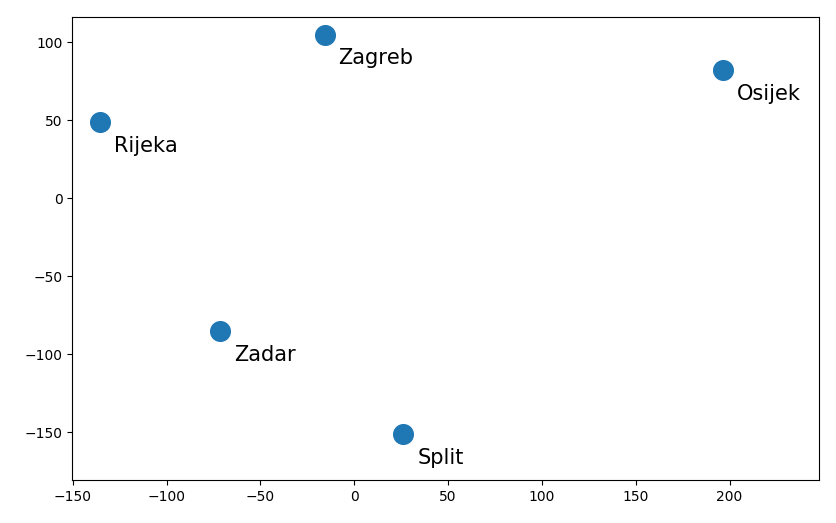
\includegraphics[width=11cm]{resources/images/reduction/mds_mapping_hr_metric.png}
    \caption{Metričko MDS preslikavanje gradova iz tablice \ref{tab:hr_cities}}
    \label{fig:mds_mapping_hr_metric}
\end{figure}


\subsubsection{Nemetrički MDS}
Nemetrički MDS \engl{Nonmetric MDS} ima glavnu razliku od metričkog a to je da pokušava sačuvati redoslijed udaljenosti originalnih podataka. Iz tog razloga traži monotonu vezu između udaljenosti u ugrađenom prostoru i sličnosti/različitosti.

Dakle budući da se nemetrički MDS fokusira na redoslijeda u podacima, za njega možemo definirati sljedeću relaciju:
\begin{equation}
    S_{ij} < S_{kl} \iff \hat{d}_{ij} < \hat{d}_{kl}
\end{equation}

Na slici \ref{fig:mds_mapping_hr_nonmetrc} vidljiv je rezultat istog primjera udaljenosti hrvatskih gradova iz tablice \ref{tab:hr_cities} ali izveden pomoću nemetričkog MDS-a.

\begin{figure}[htb]
    \centering
    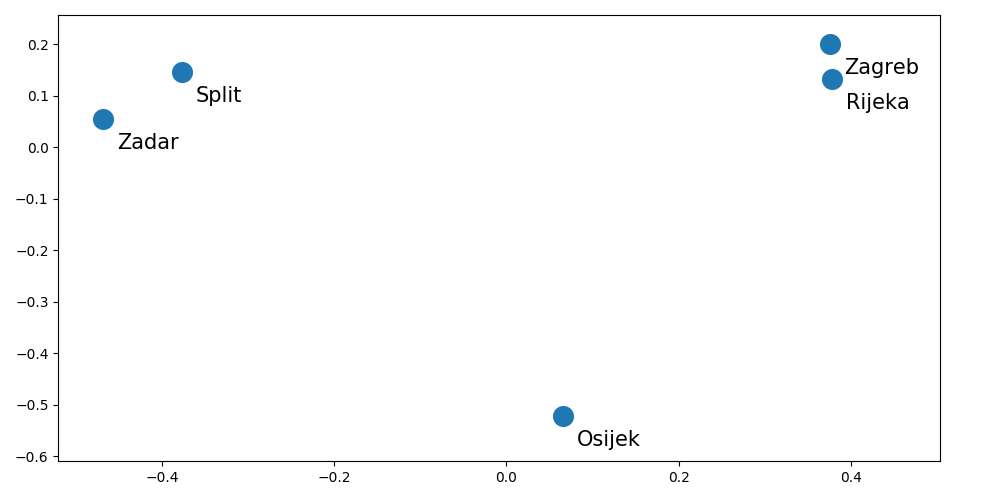
\includegraphics[width=11cm]{resources/images/reduction/mds_mapping_hr_nonmetric.png}
    \caption{Nemetričko MDS preslikavanje gradova iz tablice \ref{tab:hr_cities}}
    \label{fig:mds_mapping_hr_nonmetrc}
\end{figure}
Vidljivo je kako udaljenosti nisu zadržane ali je redoslijed gradova zadržan.

\subsection{Izometrično preslikavanje - Isomap}

Izometrično preslikavanje (engl. Isometric mapping) ili skraćeno Isomap je vrlo široko korištena metoda učenja mnogostrukosti, također jedna od najranijih. Ona je na neki način proširenje MDS-a. MDS radi preslikavanje koristeći euklidske udaljenosti parova primjera, dok Isomap koristi geodetske udaljenosti inducirane pomoću grafikona susjedstva ugrađenog u klasično skaliranje. Isomap definira geodetsku udaljenost kao zbroj težine bridova duž najkraćeg puta između dva čvora.

\begin{figure}[htb]
    \centering
    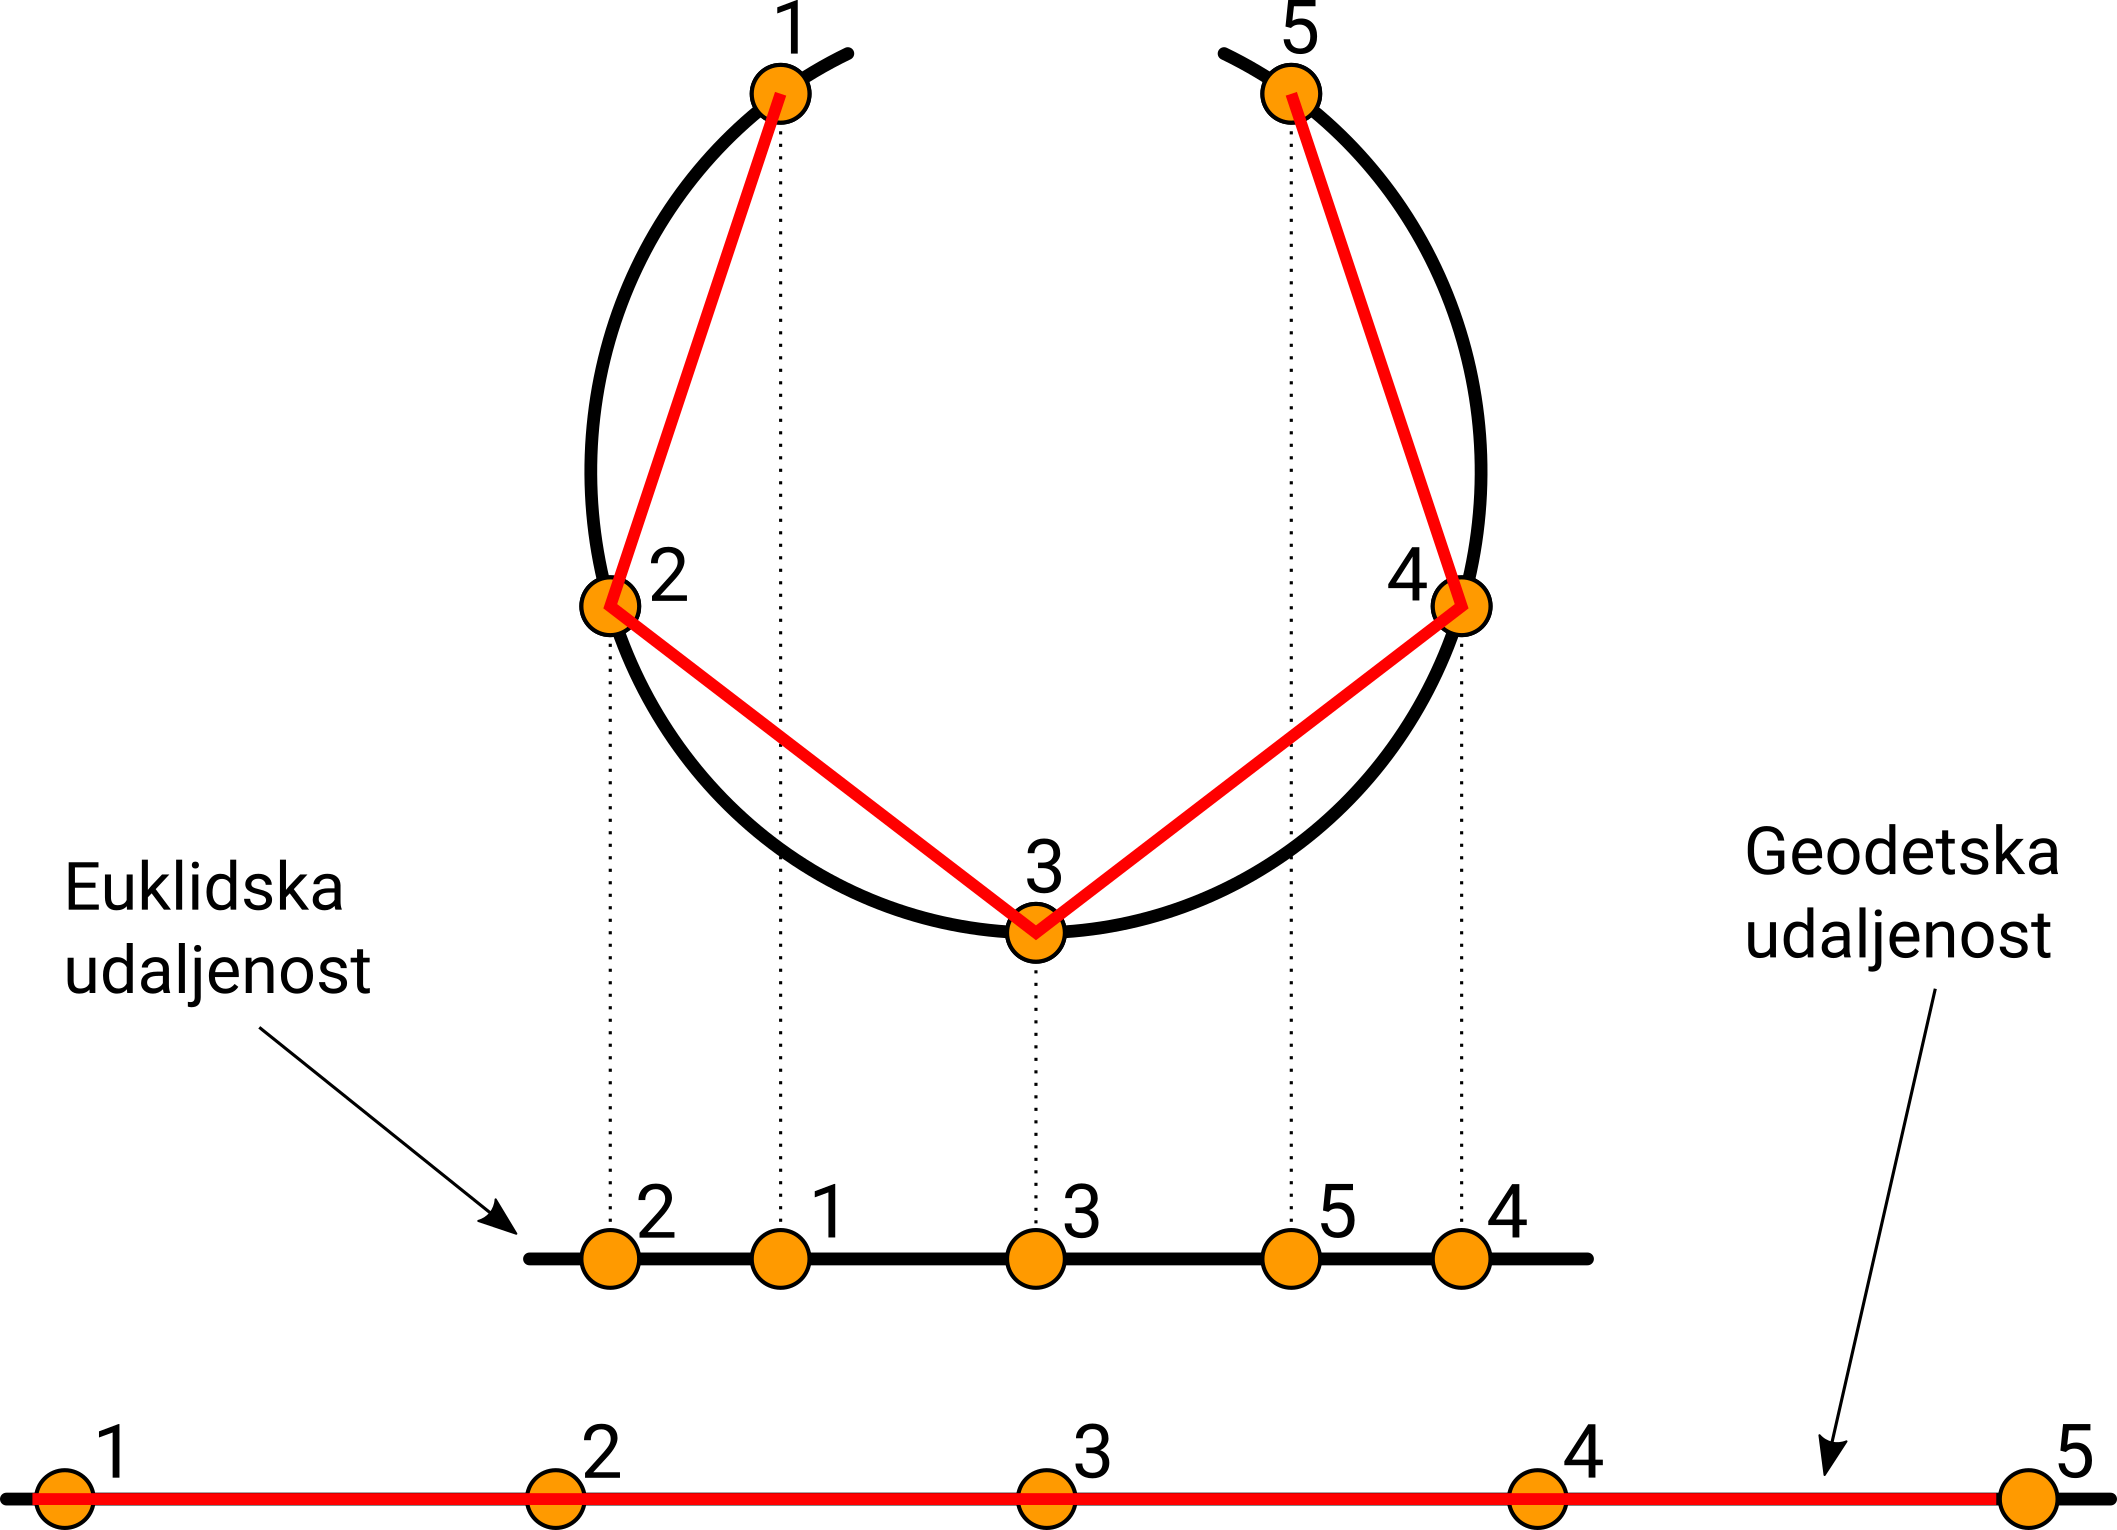
\includegraphics[width=12cm]{resources/images/reduction/euclid_vs_geodetic.png}
    \caption{Razlika između euklidske i geodetske udaljenosti}
    \label{fig:euclid_vs_geodetic}
\end{figure}

Algoritam Isomap (u najkraćim crtama):
\begin{itemize}
    \item određivanje susjednih točaka za svaku točku (npr. k-NN, ball tree\dots)
    \item izgradnja gradnja susjedstva (točke su povezane ako su susjedi, inače ne)
    \item Računanje najkraće udaljenosti između svih čvorova (npr: Dijkstra)
          \begin{itemize}
              \item[$\rightarrow$] geodetske udaljenosti
          \end{itemize}
    \item Računanje niskodimenzionalne mnogostrukosti (npr. MDS)
\end{itemize}

\bigskip
Zbog potrebe za računanje najbližih susjeda u svim točkama a zatim najkraćih udaljenosti u grafu susjednosti, Isomap je računski vrlo zahtjevan za velike skupove podataka.

\subsection{Lokalno linearno ugrađivanje - LLE}
Lokalno linearno ugrađivanje (\englnp{Locally Linear Embedding}, skrać \emph{LLE}) je algoritam za učenje mnogostrukosti koji se temelji na jednostavnim geometrijskim intuicijama; da je mnogostrukost približno linearna lokalno na djelu oko točke. On za razliku od npr. MDS-a, koji gleda globalnu struktura, gleda samo lokalnu strukturu najbližih nekoliko susjeda zbog čega se bolje skalira na veće skupove podataka (slika \ref{fig:connections}).

\begin{figure}[htb]
    \centering
    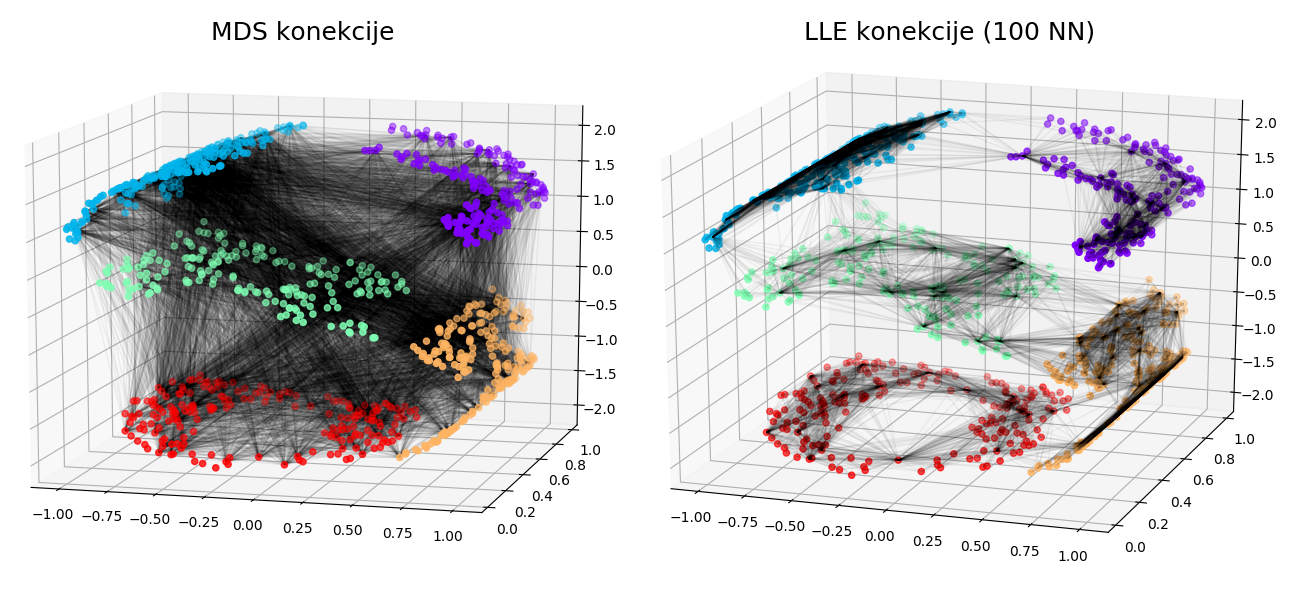
\includegraphics[width=\textwidth]{resources/images/reduction/connections.png}
    \caption{Usporedba provjerenih udaljenosti algoritmima MDS i LLE}
    \label{fig:connections}
\end{figure}

Pretpostavimo da se podaci sastoje od $N$ vektora realnih podataka $\vec{X_i}$, svaki dimenzionalnosti $D$ uzorkovanih s neke konveksne glatke temeljne mnogostrukosti. Pod uvjetom da postoji dovoljno podataka, za očekivati je da svaka točka podataka i njezini susjedi leže na ili vrlo blizu malog lokalno linearnog dijela temeljne mnogostrukosti. Tada se geometrija tog malog djela prostora može karakterizirati linearnom kombinacijom, tj. linearnim koeficijentima koji rekonstruiraju svaku točku iz svojih susjeda.

U najjednostavnijoj inačici LLE algoritma, prvi korak je odrediti lokalno susjedstvo točaka, to se radi pomoću algoritma k najbližih susjeda. Pogrešku rekonstrukcije tada možemo mjeriti pomoću funkcije gubitka koju jednostavno definiramo kao:
\begin{equation}
    \epsilon(W) = \sum_i \vert{\vec{X_i} - \sum_{j \in N(i)} W_{ij} \vec{X_j}}^2
    \label{eq:lle1}
\end{equation}
gdje je $N(i)$ susjedstvo od $X_i$.\\
Minimizacijom gubitka $\epsilon$ zatim se mogu odrediti težine $W$.

Konačno, koristeći dobivene težine, određuje se niskodimenzionalni vektori $\vec{Y_i}$ koji predstavljaju mapiranu vrijednost originalnih podataka opisanih vektorima $\vec{X_i}$. To se radi tako da se minimizira gubitak koji definiramo sljedećom jednadžbom:
\begin{equation}
    \Phi(Y) = \sum_i \vert{\vec{Y_i} - \sum_{j} W_{ij} \vec{Y_j}}^2
    \label{eq:lle2}
\end{equation}

Algoritam LLE (u najkraćim crtama):
\begin{itemize}
    \item Odrediti susjede svake točke vektora $\vec{X_i}$
    \item Izračunati težine $W_{ij}$ koje najbolje rekonstruiraju svaku točku $\vec{X_i}$ iz svojih susjeda minimizirajući funkciju gubitka $\epsilon$ definiranu jednadžbom \ref{eq:lle1}
    \item Izračunati vektore $\vec{Y_i}$ koji su najbolja rekonstrukcija pomoću težina $W_{ij}$ minimizirajući funkciju gubitka $\Phi$ definiranu jednadžbom \ref{eq:lle2}
\end{itemize}

\begin{figure}[htb]
    \centering
    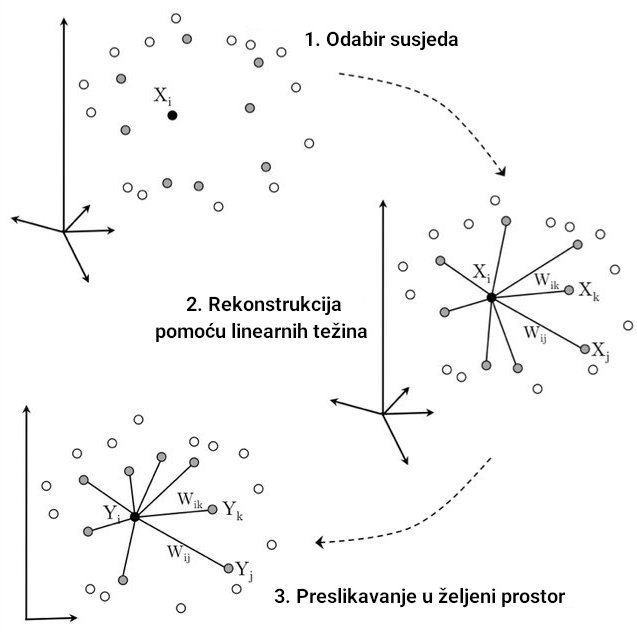
\includegraphics[width=12cm]{resources/images/reduction/lle_steps.jpg}
    \captionsource{Ilustracija algoritma LLE}{\cite{saul2003think}}
    \label{fig:lle_steps}
\end{figure}

Pokazalo se kako LLE nije uvijek stabilan. Kada je broj susjeda veći od broja ulaznih dimenzija, matrica koja definira svako lokalno susjedstvo je nedovoljnog ranga.
\newpage

\subsection{Modificirano lokalno linearno ugrađivanje - MLLE}

Modificirano lokalno linearno ugrađivanje (\englnp{Modified Locally Linear Embedding}, skrać. \emph{MLLE}) je poboljšanje LLE algoritma koji su predložili \cite{zhang2007mlle}, te je pokušaj rješavanja problema regularizacije LLE metode. MLLE to radi tako da za svaku točku koristi linearnu kombinaciju \emph{više} vektora $\vec{W_{i}}$ za rekonstrukciju točke $\vec{X_i}$ u kontrastu sa samo jednim metode LLE. Ovom jednostavnom metodom uspješno se postiže veća stabilnost ugrađivanja.

\subsection{Hessijsko svojstveno preslikavanje - HLLE}

Hessijsko svojstveno preslikavanje (engl. Hessian Eigenmapping) također poznato kao LLE baziran na Hessijanu (skrać. HLLE) je još jedna metoda rješavanja regularizacijskog problema od LLE algoritma, dosadašnju pretpostavku konveksnosti mnogostrukosti. Ovaj algoritam se bazira na kvadratnoj formi $\mathcal{H}(f) = \int_M H_f(m)\|_F^2 dm$ definiranoj na funkciji $f: M \mapsto \mathbb{R}$. Ovdje $H_f$ označava Hessijana od $f$. Za definiranje Hessijana, koriste se ortogonalne koordinate na tangentnom prostoru od $M$ \citep{Donoho5591}. Taj Hessijan se koristi u svakom susjedstvu za rekonstrukciju lokalne linearne strukture.
\begin{equation}
    \mathcal{H}_{i,j} = \sum_l \sum_r ((H^l)_{r,i}(H^l)_{r,j})
\end{equation}


\subsection{Spektralno ugrađivanje - SE}
Spektralno ugrađivanje \engl{Spectral embedding} je tehnika ugrađivanja mnogostrukosti u niskodimenzionalni prostor koja koristi spektar (vlastite vrijednosti) matrice sličnosti. Ova metoda dolazi iz polja multivarijatne statistike i grupiranja podataka te se često koristi za određivanje  grupa u podacima zbog čega se još i naziva Spektralno grupiranje \engl{Spectral clustering}. Algoritam se sastoji od tri bitna koraka \citep{belkin2003laplacian}:
\begin{itemize}
    \item Izrađivanje matrice sličnosti pomoću težinskog grafa susjedstva (npr. k-NN) $\rightarrow A$
    \item Određivanje Laplacove matrice $L = D - A$, gdje je $D$ matrica stupnjeva grafa susjedstva
    \item Dekompozicija svojstvenih vrijednosti \engl{Eigenvalue decomposition}
\end{itemize}

\subsection{Lokalno tangentno poravnanje prostora - LTSA}

Lokalno tangentno poravnanje prostora (\englnp{Local Tangent Space Alignment}, skrać. \emph{LTSA}) je metoda za pronalaženje ugrađene mnogostrukosti koja je vrlo slična metodi LLE (i izvedenim metodama kao HLLE i MLLE) te je bazirana na istoj pretpostavci, lokalne linearnosti. No ova metoda, kao što je vidljivo iz imena, oslanja se na koncept tangentnog prostora $T_xM$ mnogostrukosti $M$ u točki $x$. Ukoliko bi se neki objekt kretao po mnogostrukosti u točki $x$ bi imao neki vektor brzine koji je tangentan prostoru, drugim riječima to je tangentni vektor. Skupina takvih vektora iz mogućih krivulja koje prolaze kroz točku $x$ definiraju tangentni prostor u njoj. Za 2D mnogostrukost ugrađenu u 3D prostor tangentni prostor bi bio ravnina (slika \ref{fig:tanget_space}).

\bigskip
\begin{figure}[htb]
    \centering
    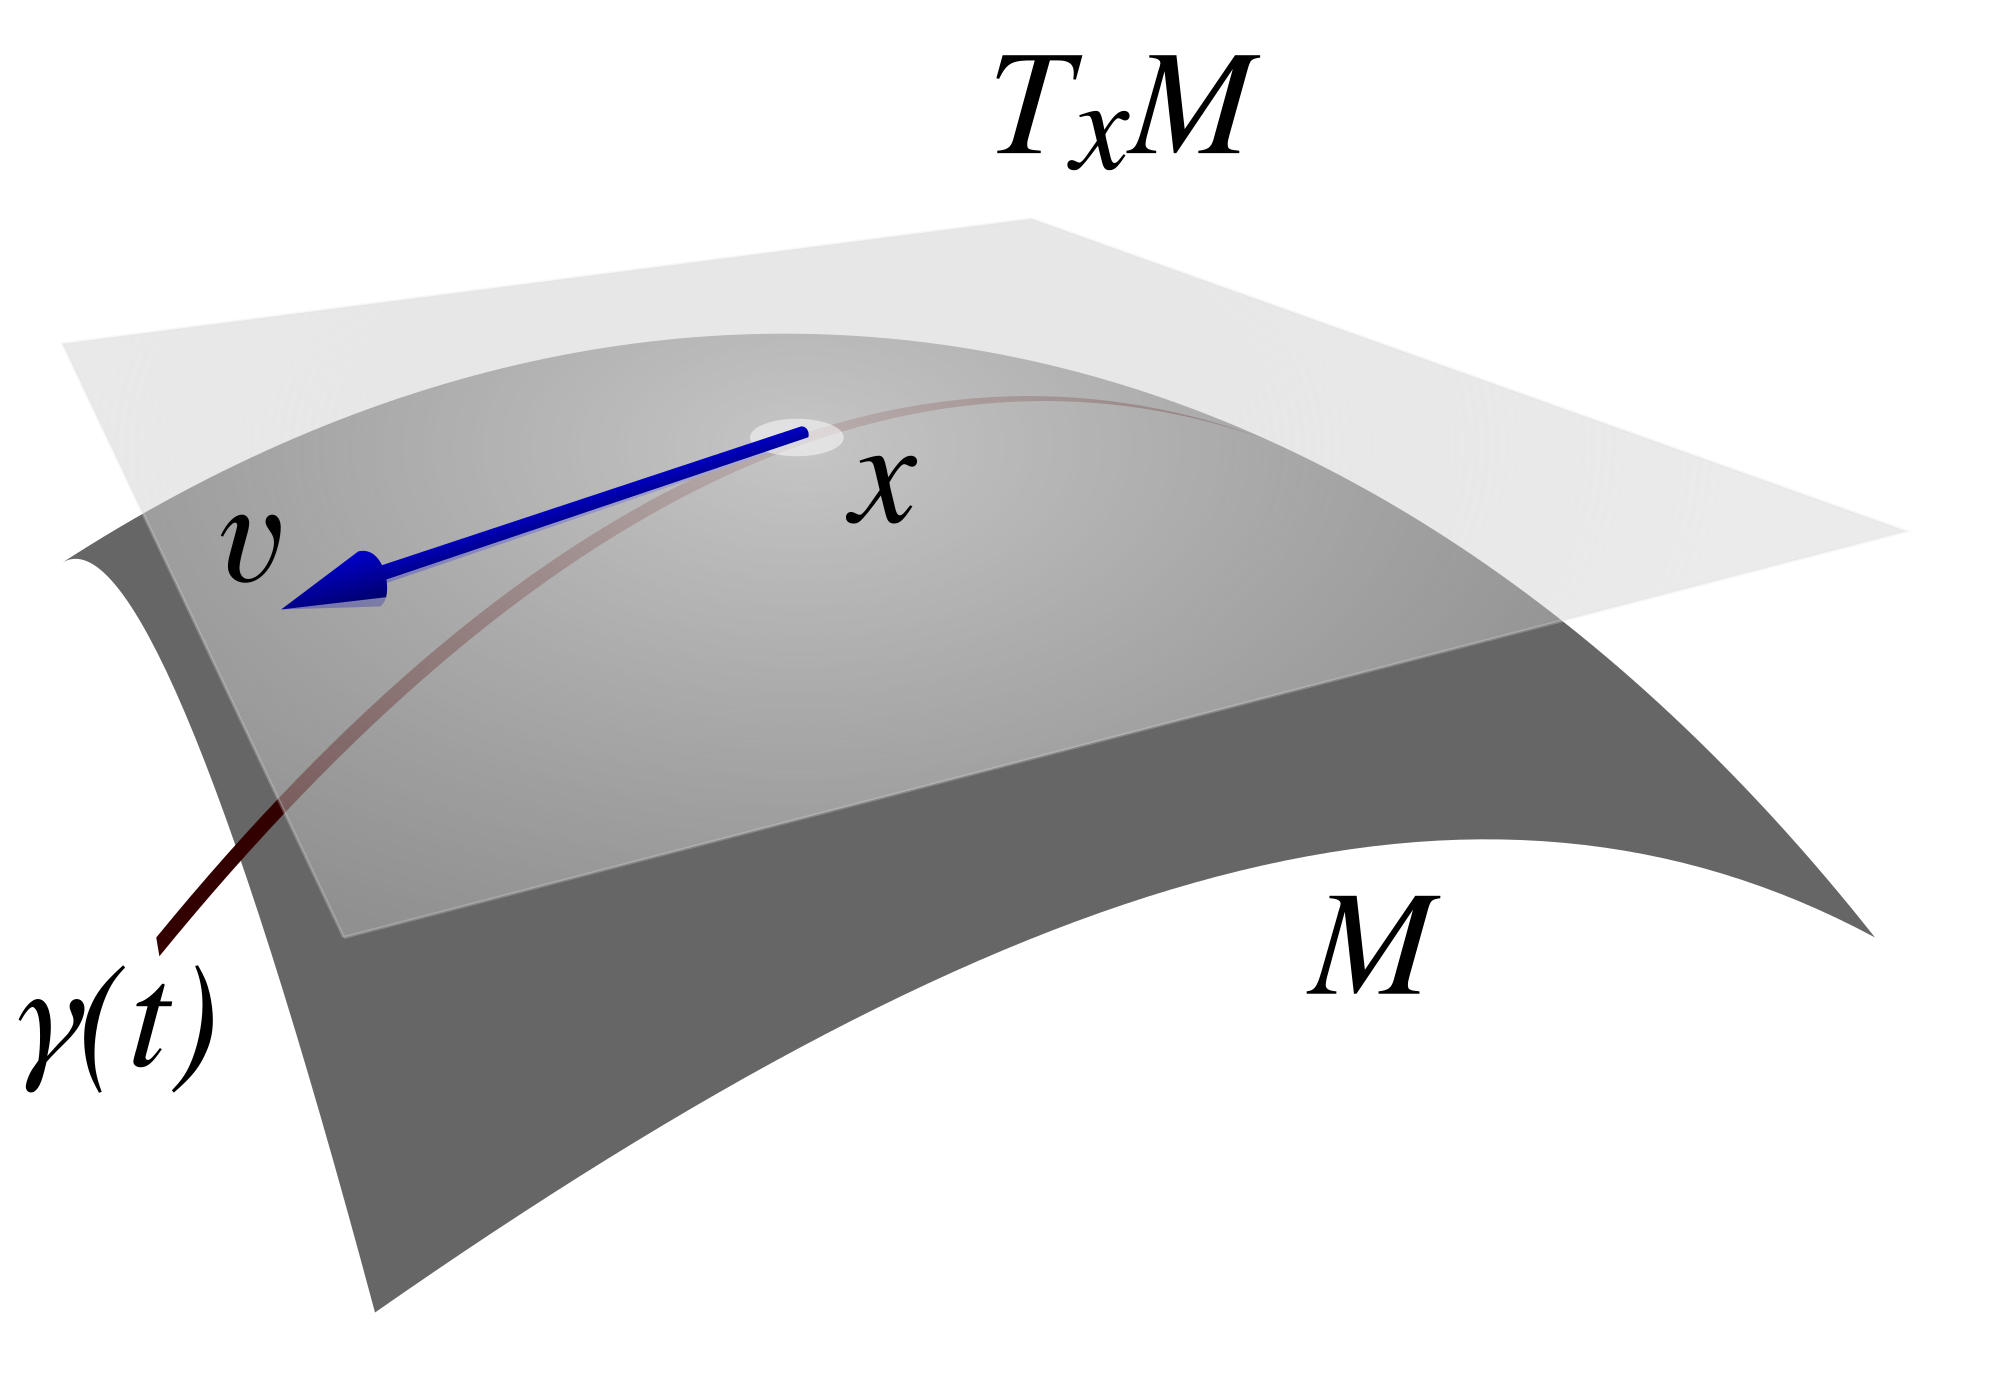
\includegraphics[width=10cm]{resources/images/reduction/tanget_space.png}
    \captionsource{Tangentni prostor $T_{x}M$ i tangentni vektor $v \in T_{x}M$, na krivulji koja prolazi $ x \in M$.}{\cite{wikimedia2008tangent}}
    \label{fig:tanget_space}
\end{figure}
\bigskip

Ideja LTSA je da postoji linearno preslikavanje iz visokodimenzionalnog prostora u kojem leže originalni podaci u njegov lokalni tangentni prostor i da za odgovarajući niskodimenzionalni prostor postoji preslikavanje u isti taj lokalni tangentni prostor. Za LTSA i HLLE pokazano je da su matematički vrlo slični uz sine razlike, poput toga da LTSA uključuje trenutnu točku u susjedstvo, dok HLLE ne, te da iako koriste različite metode za rješavanje jednadžbe poravnanja, rješenje je jednako ako se uzme da HLLA koristi isti način izgradnje susjedstva kao LTSA \citep{7837655}


\subsection{Ugradnja pomoću t-distribuiranog stohastičkog susjeda -\\ t-SNE}
Ugradnja pomoću t-distribuiranog stohastičkog susjeda (engl. t-distributed Stochastic Neighbor Embedding, skrać. t-SNE) relativno je novija traži nižedimenzionalnu strukturu tako da svojstva grupiranja ostanu sačuvana gradeći neizrazitu \engl{fuzzy} topološku strukturu. Ovu metodu su objavili su \cite{maaten2008visualizing} kao metodu za vizualizaciju podataka visokodimenzionalnih podataka tako da se svakoj točki da lokacija u dva ili tri dimenzijskoj mapi. To radi tako da pretvara srodstvo točaka u vjerojatnosti. Srodstva u izvornom prostoru predstavljena su Gaussovim zajedničkim vjerojatnostima, dok u ugrađenom prostoru su predstavljeni t-razdiobama. t-SNE metoda je varijacija ugrađivanja stohastičkog susjeda \engl{Stochastic Neighbor Embedding} koja je puno jednostavnija za optimizaciju te pruža vizualno puno bolje rezultate tako što smanjuje tendenciju podataka da se gomilaju u centru mape.
\begin{figure}[htb]
    \centering
    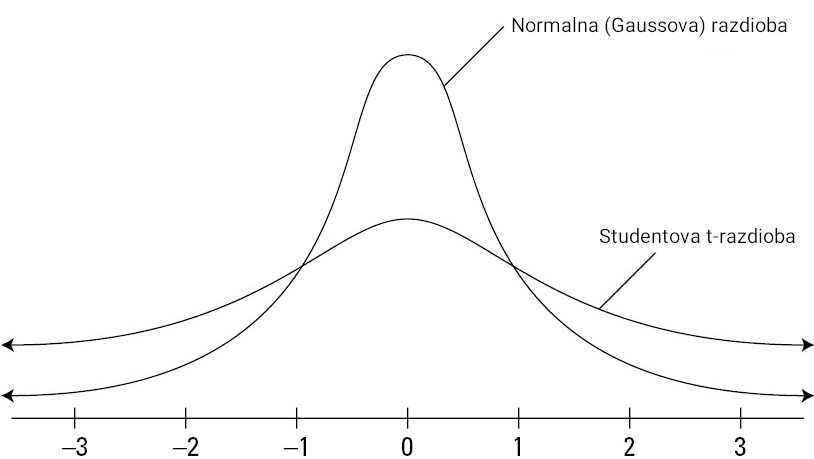
\includegraphics[width=9cm]{resources/images/reduction/tsne.jpg}
    \caption{Prikaz Normalne (Gaussove) razdiobe i Studentov t-razdiobe}
    \label{fig:tsne}
\end{figure}

t-SNE koristi Studentovu t-razdiobu za dobiveni prostor a ne Normalnu kao za originalni prostor, što je zato što Normalna razdioba ima vrlo male vjerojatnosti pri rubovima (vidljivo na slici \ref{fig:tsne}), te bi se podaci zgušnjavali prema sredini grupe. Dok Studentova t-razdioba nema taj problem te to omogućuje da t-SNE bude posebno osjetljiv na lokalnu strukturu.

Kako bismo dobili distribuciju u ugrađenom prostoru Kullback-Leiblerova divergencija zajedničkih vjerojatnosti u izvornom prostoru i ugrađenom prostoru se minimizirana gradijentnim spustom. Treba primijetiti da KL divergencija nije konveksna, stoga je ponekad korisno program pokrenuti više puta koristeći drugo sjeme za ostvarenje slučajnosti. t-SNE je računalno vrlo zahtjevan te na uzorku s puno primjera potrebno je i nekoliko sati da završi, te se iz tog razloga i svoje svojstvenosti da sačuva grupiranje uglavnom koristi za vizualizaciju podataka.

\subsection{Uniformna aproksimacija i projekcija mnogostrukosti -\\ UMAP}

Posljednja velika metoda u redukciji dimenzionalnosti, objavljena je od strane \cite{mcinnes2018umap} te pruža iznimne rezultate vizualno slične onima od t-SNE metode ali, zbog svoje snažne matematičke pozadine, ima mogućnost generalizacije na neviđenim podacima. Također UMAP metoda se puno bolje skalira s podacima te je na, primjerice, skupu podataka "GoogleNews" 19 puta brža od t-SNE metode čije izvođenje traje 4.5 sati dok UMAP isti posao odradi u 14 minuta. Doduše, ova metoda pretpostavlja dva svojstva; da su podaci uniformno distribuirani i da je mnogostrukost lokalno povezana. Drugo svojstvo ne znači da je potrebno da cijela mnogostrukost bude povezana, već samo da ne postoji npr. točka koja je sama udaljena od svih. Ova pretpostavka je razumna za podatke iz stvarnog svijeta. Što se uniformnosti tiče, kako bi se osiguralo korisnik mora biti svjestan ovoga te po potrebi napraviti pretprocesiranje početnog skupa podataka. Kao i t-SNE, ali i mnogo metoda navedenih u ovom radu, UMAP gradi graf susjedstva. Za to koristi stabla slučajnih projekcija (\englnp{Random projection trees}, skrać. \emph{RP-trees}) i spustom najbližih susjeda (\englnp{Nearest Neighbor Descent}, skrać. \emph{NN-descent}). Ovi vrlo efikasni algoritmi omogućuju brz pronalazak najbližih susjeda i izgradnju grafa.

Umjesto Studentove t-distribucije za modeliranje udaljenosti u niskodimenzionalnom prostoru, UMAP koristi sličnu obitelj krivulja definiranu sljedećom jednadžbom:
\begin{equation}
    q_{ij} = (1 + a(y_i - y_j)^{2b})^{-1}
\end{equation}
A parametre $a$ i $b$ pronalazi pomoću nelinearne regresije najmanjih kvadrata na dijelovima funkcije.

Također, UMAP koristi binarnu unakrsnu entropiju (\ref{eq:binCE}) kao funkciju gubitka umjesto KL divergencije kao što to t-SNE radi.
\begin{align}
    CE(X, Y) & = \sum_i \sum_j \left[ p_{ij}(X) \log \left( \frac{p_{ij}(X)}{q_ij(Y)} \right)
    \right. \nonumber                                                                         \\ &\hphantom{ \sum_i \sum_j \big[} + \left.
        ( 1 - p_{ij}(X)) \log \left(\frac{1 - p_{ij}(X)}{1 - q_{ij}(Y)}\right) \right]
    \label{eq:binCE}
\end{align}
Laički rečeno, prvi član unutar sume omogućuje mapiranje grupa ispravno, dok drugi član omogućuje mapiranje razmaka ispravno zbog čega  UMAP može opisati globalnu strukturu.

Konačno, umjesto gradijentog spusta (GD), UMAP koristi stohastički gradijentni spust (SGD) što ujedno ubrzava vrijeme izvođenja i zahtjeva manje memorije.

\section{Usporedba algoritama za učenje mnogostrukosti}

Iako matematika priča zanimljivu priču o navedenim algoritmima, kako bi se najbolje ilustrirale njihove sličnosti, različitosti i granice u ovom poglavlju uspoređivat će se kako pojedini algoritmi rade na određenim primjerima.

U prvom djelu poglavlja bit će napravljen jednostavan ilustrativni primjer. Kako bi se to izvelo za definiranje mnogostrukosti će biti napravljeno suprotno od zadatka učenja mnogostrukosti, točnije prvo će se definirati mnogostrukost u dvodimenzionalnom prostoru, a zatim će se ona ugraditi u trodimenzionalni prostor. Na ovaj način od algoritama za redukciju dimenzionalnosti imamo dobro definiran cilj; "poništiti" ugradnju, tj. želimo da rezultat redukcije bude originalna mnogostrukost. Ugrađivanje će biti izvedeno koristeći linearnu i nelinearnu transformaciju kako bi se pokazale razne težine ugrađivanja.

Originalna dvodimenzionalna mnogostrukost (vidljiva na slici \ref{fig:ferko}) definirana je podacima u obliku riječi „FERKO”, gdje će svako slovo dobiti svoju zasebnu klasu (to će biti prikazano pomoću boje). Taj primjer odabran je kako bi se lako vidjelo bilo kakvo izobličenje, te da se rotacije i zrcaljenja jasno vide.

Također, radi provjere pristranosti algoritama, jedan primjer koji će biti korišten jesu slučajno generirani podaci.

Drugi dio poglavlja prikazat će usporedbu primjera na stvarnom skupu podataka, gdje mnogostrukost unaprijed nije poznata. Skup korišten u ovom radu je skup modnih artikala "Fashion-MNIST" koji se sastoji od crno bijelih slika veličine 28x28 razvrstanih u 10 razreda, svaki za jedan artikal. Broj susjeda koji koristimo bit će 100 za sve primjere.

\begin{figure}[htb]
    \centering
    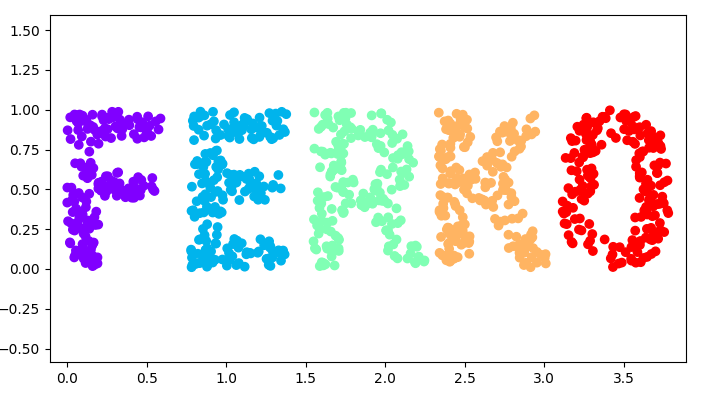
\includegraphics[width=12cm]{resources/images/reduction/compare/ferko.png}
    \caption{Dvodimenzionalna mnogostrukost}
    \label{fig:ferko}
\end{figure}

\paragraph{Primjer 1.}
Prvi primjer korišten u ovom radu je spomenuta mnogostrukost sa slike \ref{fig:ferko}, ali ugrađena u trodimenzionalni prostor koristeći linearnu transformaciju. To je postignuto projiciranjem mnogostrukosti koristeći metodu slučajne projekcije. Rezultantna mnogostrukost prikazana je na slici \ref{fig:ferko3d}

\begin{figure}[htb]
    \centering
    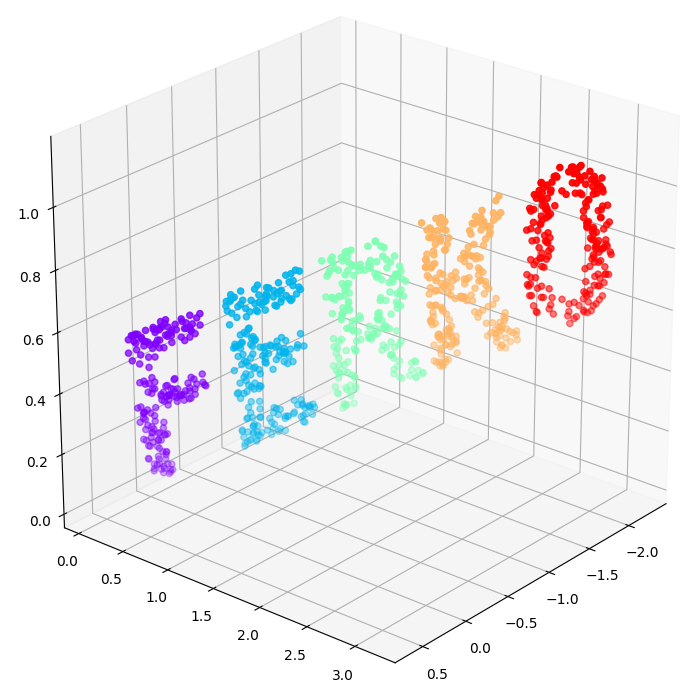
\includegraphics[width=6.5cm]{resources/images/reduction/compare/ferko3d.png}
    \caption{Mnogostrukost ugrađena u trodimenzionalni prostor}
    \label{fig:ferko3d}
\end{figure}

Na ovako jednostavnom primjeru očekivano je da svi algoritmi osim algoritama t-SNE i UMAP uspješno pronađu mnogostrukost. Zašto ne t-SNE i UMAP? Oni se razlikuju od ostalih algoritama za učenje mnogostrukosti tako što ne pokušavaju zadržati topologiju, već svojstva grupa. Iz tog razloga za očekivati je da će t-SNE i UMAP grupirati točke u zasebne grupe, svaku za svoje slovo, ali da će i dalje udaljenosti slova ostati slične. Dakle da će slovo F biti najdalje slovu O ( točnije da će ljubičasta grupa biti najdalje crvenoj grupi). Rezultati za sve algoritme vidljivi su na slici \ref{fig:x3d}.

Kao što je bilo očekivano većina algoritama uspješno je naučila mnogostrukost na do skaliranje, rotaciju i zrcaljenje u ovom primjeru, mogu se primijetiti samo mali defekti na slovu F kod Isomap algoritma. No vidljivo je da spektralno ugrađivanje (grupiranje), t-SNE i UMAP nisu rekonstruirali originalnu mnogostrukost. To je zato što su ti algoritmi namijenjeni za pronalaženje grupa u visokodimenzionalnom prostoru i preslikavanju tih grupa u niskodimenzionalni. Ali kod oba algoritma može se primijetiti da su zadržani odnosi između grupa. Kao što je prije bilo očekivano grupe koje su prije bile najdalje i dalje jesu, tj. može se vidjeti da klase i dalje idu istim redoslijedom (ljubičasta do crvena) ali ne nužno u istom smjeru. Također kod t-SNE i UMAP algoritama postoje oblici koji donekle liče na originalna slova.

\begin{figure}[htb]
    \centering
    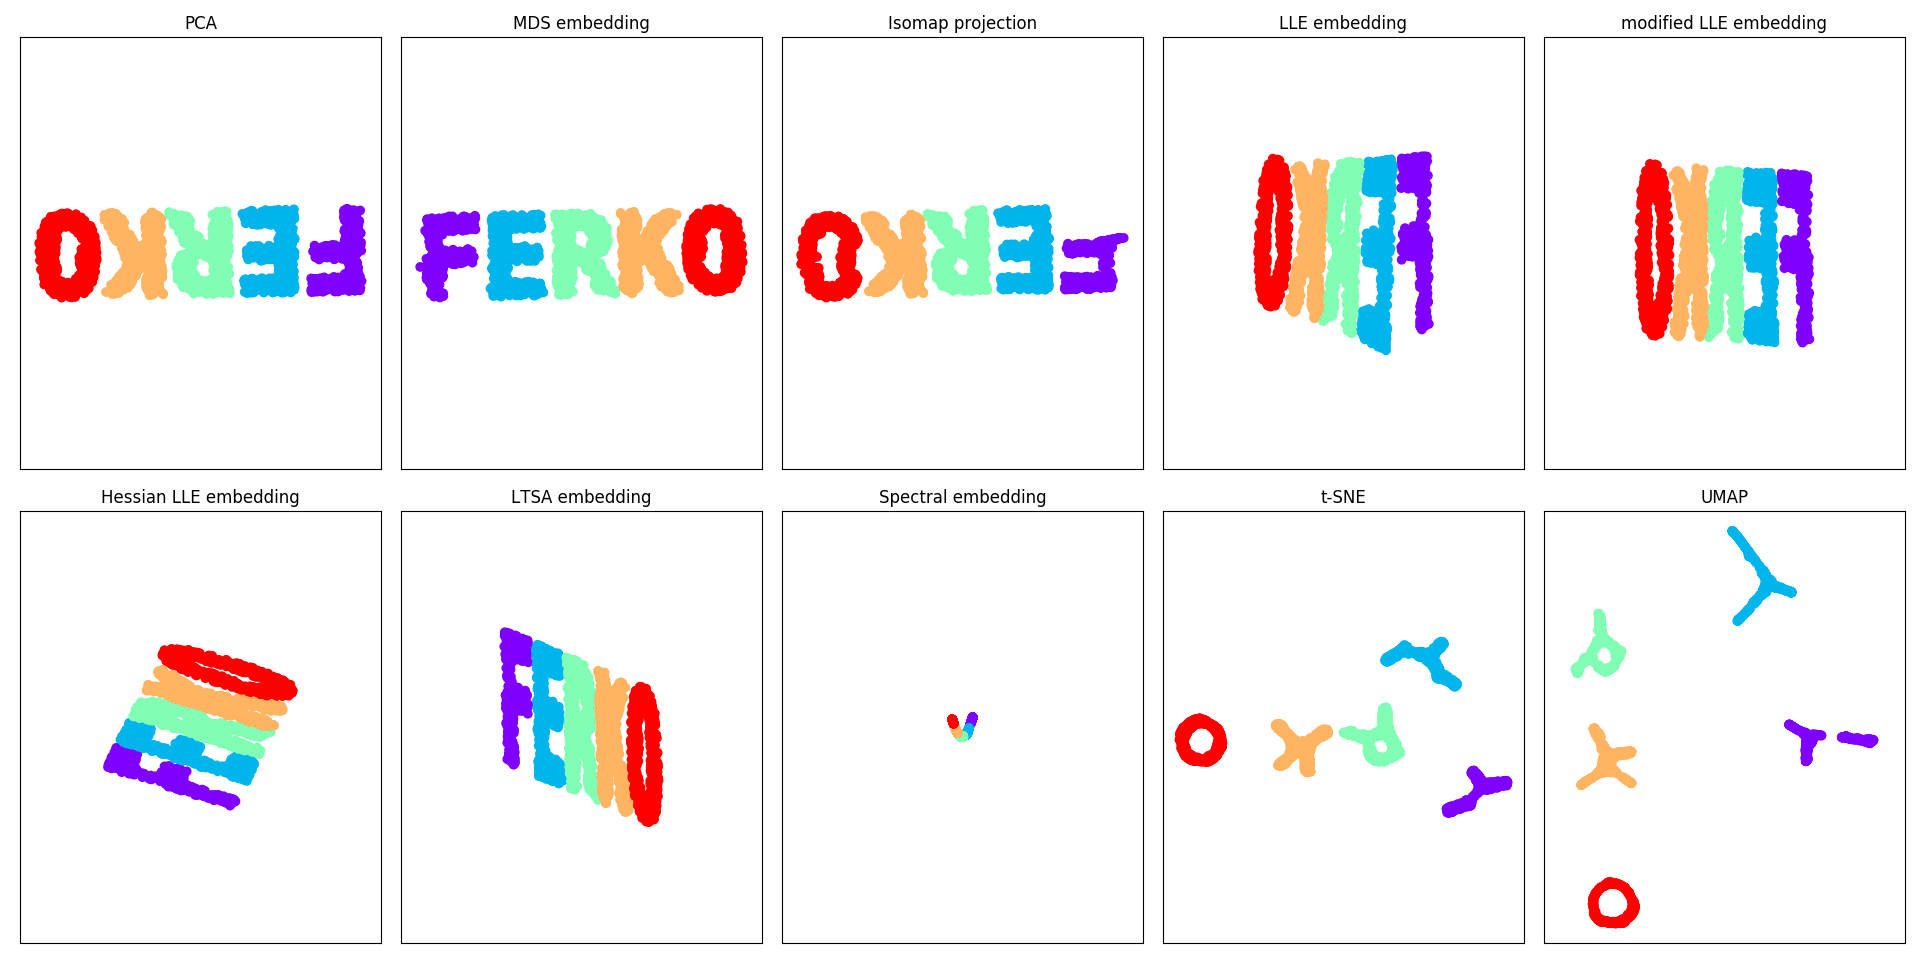
\includegraphics[width=\textwidth]{resources/images/reduction/compare/x3d.png}
    \caption{Prikaz rezultata algoritama za učenje mnogostrukosti na linearnom primjeru}
    \label{fig:x3d}
\end{figure}

\paragraph{Primjer 2.} Prošli primjer bio je vrlo jednostavan linearan primjer no kako bi uspješno bile demonstrirane prednosti nekih algoritama nad drugima potrebno je pogledati malo složeniji primjer. Iz tog razloga, primjer dva koristi mnogostrukost "savinutu" u oblik slova "S" i takvu ugraditi u trodimenzionalni prostor. Ovako definirana mnogostrukost vizualizirana je na slici \ref{fig:ferkoS}.

\begin{figure}[htb]
    \centering
    \includegraphics[width=\textwidth]{resources/images/reduction/compare/ferkoS.png}
    \caption{Mnogostrukost u obliku slova "S" ugrađena u trodimenzionalni prostor (iz dvije različite perspektive)}
    \label{fig:ferkoS}
\end{figure}

Mnogostrukost je postignuta transformacijom koju definiraju sljedeće relacije:
\begin{align}
     & \vec{t} = 0.75 \pi \cdot (\vec{x} - 2);
    \\
     & \vec{x'} = \sin(\vec{t});
    \\%;\quad
     & \vec{y'} = \vec{y};
    \\%;\quad
     & \vec{z'} = sign(\vec{t}) \cdot (\cos(\vec{t}) - 1)
    \label{eq:makeS}
\end{align}

\bigskip
Na ovakvom primjeru očekujemo da neće svi algoritmi uspješno pronaći ugrađenu mnogostrukost. Jedna od takvih metoda zasigurno je PCA koja zbog svoje linearne prirode ne može definirati odgovarajuću transformacijsku funkciju potrebnu za željeno mapirane u dvodimenzionalni prostor. Dodatno, očekivano je i za MDS da će imati poteškoće u transformaciji zbog korištenja euklidskih udaljenosti umjesto geodetskih što je vizualno opisano na slici \ref{fig:euclid_vs_geodetic}. Za LLE je teško predvidjeti rezultat zbog velike ovisnosti algoritma o broju najbližih susjeda koji se koriste. Te nedostatke rješavaju MLLE i HLLE algoritmi od kojih dakle očekujemo da uspješno riješe ovaj problem. Očekivano ponašanje algoritma LTSA je slično onome od algoritma HLLE zbog matematičke sličnosti dviju metoda. Za spektralno ugrađivanje, t-SNE i UMAP ne bi trebala postojati velika razlika u pristupu ova dva primjera zbog čega očekujemo slične rezultate kao i prije.

\begin{figure}[htb]
    \centering
    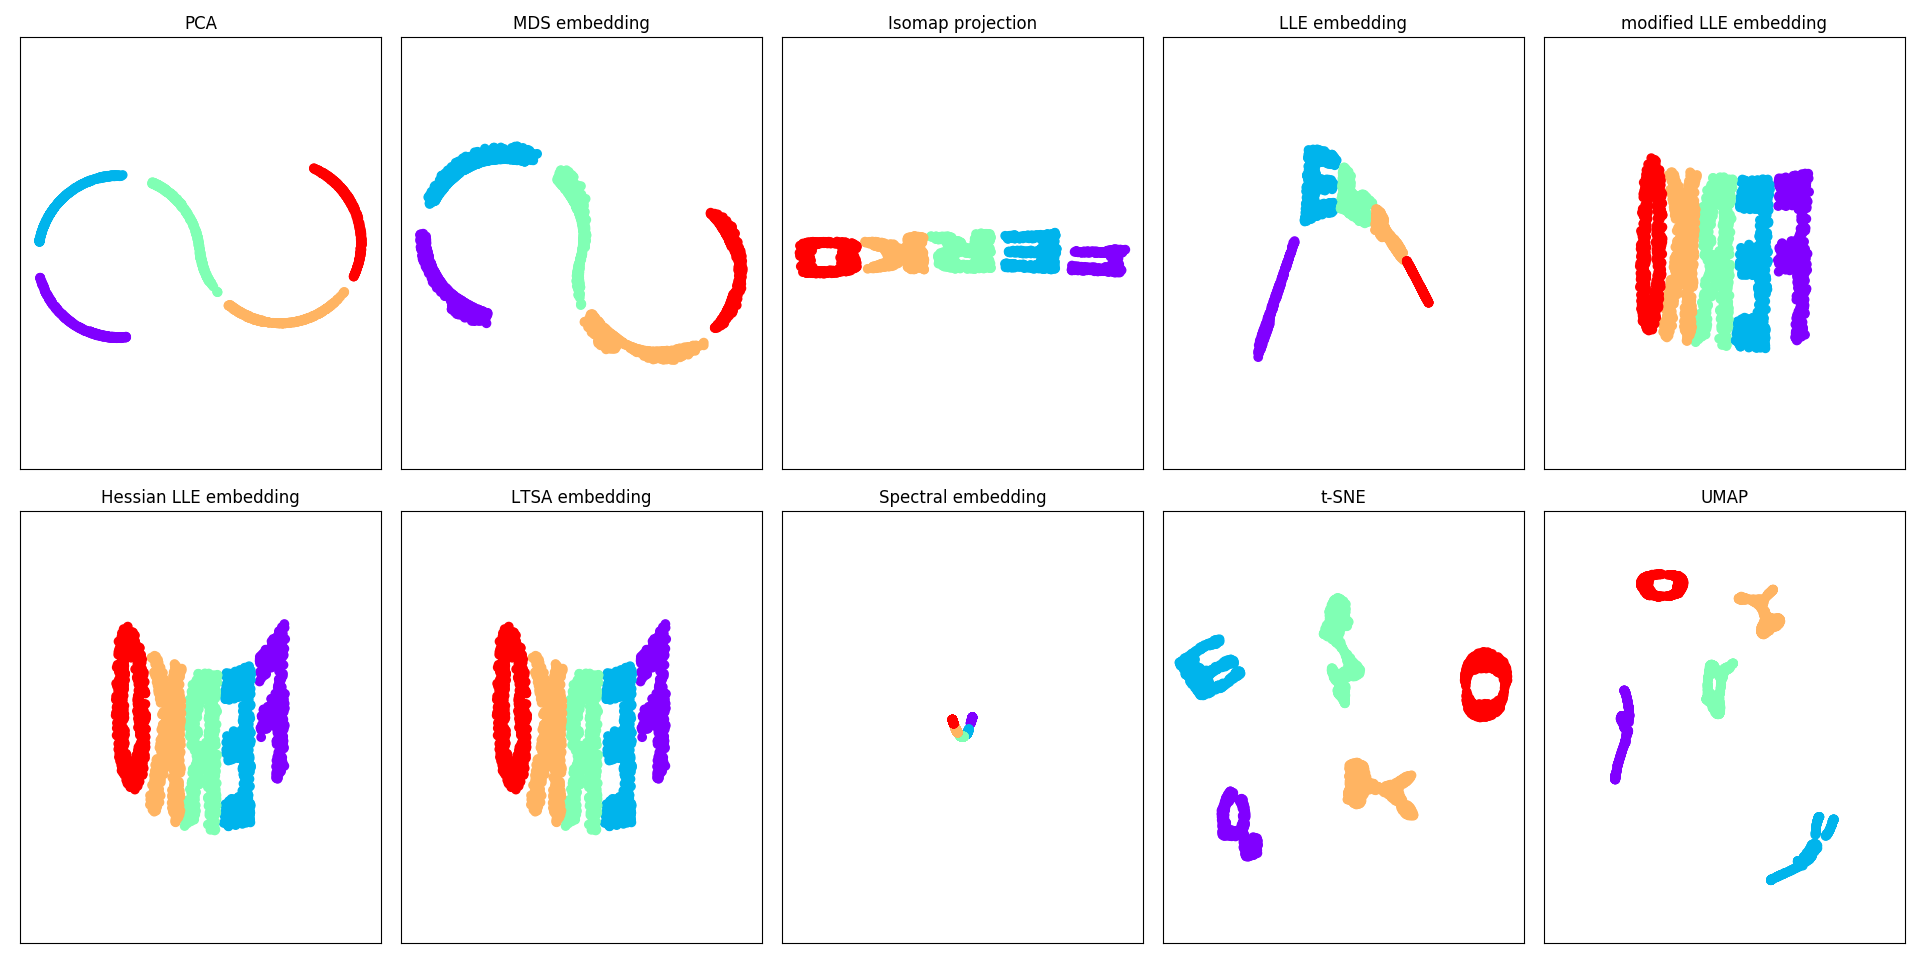
\includegraphics[width=\textwidth]{resources/images/reduction/compare/xs.png}
    \caption{Prikaz rezultata algoritama za učenje mnogostrukosti na nelinearnom (S) primjeru}
    \label{fig:xs}
\end{figure}

Iz ovog rezultata primjera (slika \ref{fig:xs}), za PCA algoritam možemo vidjeti da iako nije uspješno odredio ugrađenu mnogostrukost, uspješno je odredio smjerove dviju najvećih varijanci u podacima. Također su vidljivi nedostaci MDS algoritma. Kako bi zadržao odnose euklidske udaljenosti MDS je odbacio y os. Isto tako vidljivo je značajno poboljšanje koje geodetske udaljenosti korištene u Isomap algoritmu donose. Problem regularizacije vrlo je očit u rezultatu LLE algoritma, ali vidljivo je i značajno poboljšanje koje donose modifikacije algoritama MLLE i HLLE. Algoritam LTSA očekivano je sličan algoritmu HLLE i očekivano je uspješan u ovom problemu. t-SNE i Spektralno ugrađivanje, t-SNE i UMAP rezultirali su s gotovo jednakim rezultatima kakvi su bili na prošlom primjeru, što je bilo i za očekivati.


\paragraph{Primjer 3.}
S ciljem utvrđivanja postoji li pristranost u algoritmima, dobra je praska provjeriti kako se ti algoritmi ponašaju na slučajno generiranim podacima. Naravno za ovakav primjer očekujemo da algoritmi ne pronađu nikakvu ugrađenu mnogostrukost te da rezultantni nižedimenzionalni prostor izgleda jednako slučajan. Algoritmi koji održavaju svojstva grupa, kao što su spektralno ugrađivanje, t-SNE i UMAP mogli bi unijeti svoju pristranost prema grupiranju točaka. Rezultati ovog primjera vidljivi su na slici \ref{fig:xr}.

\begin{figure}[htb]
    \centering
    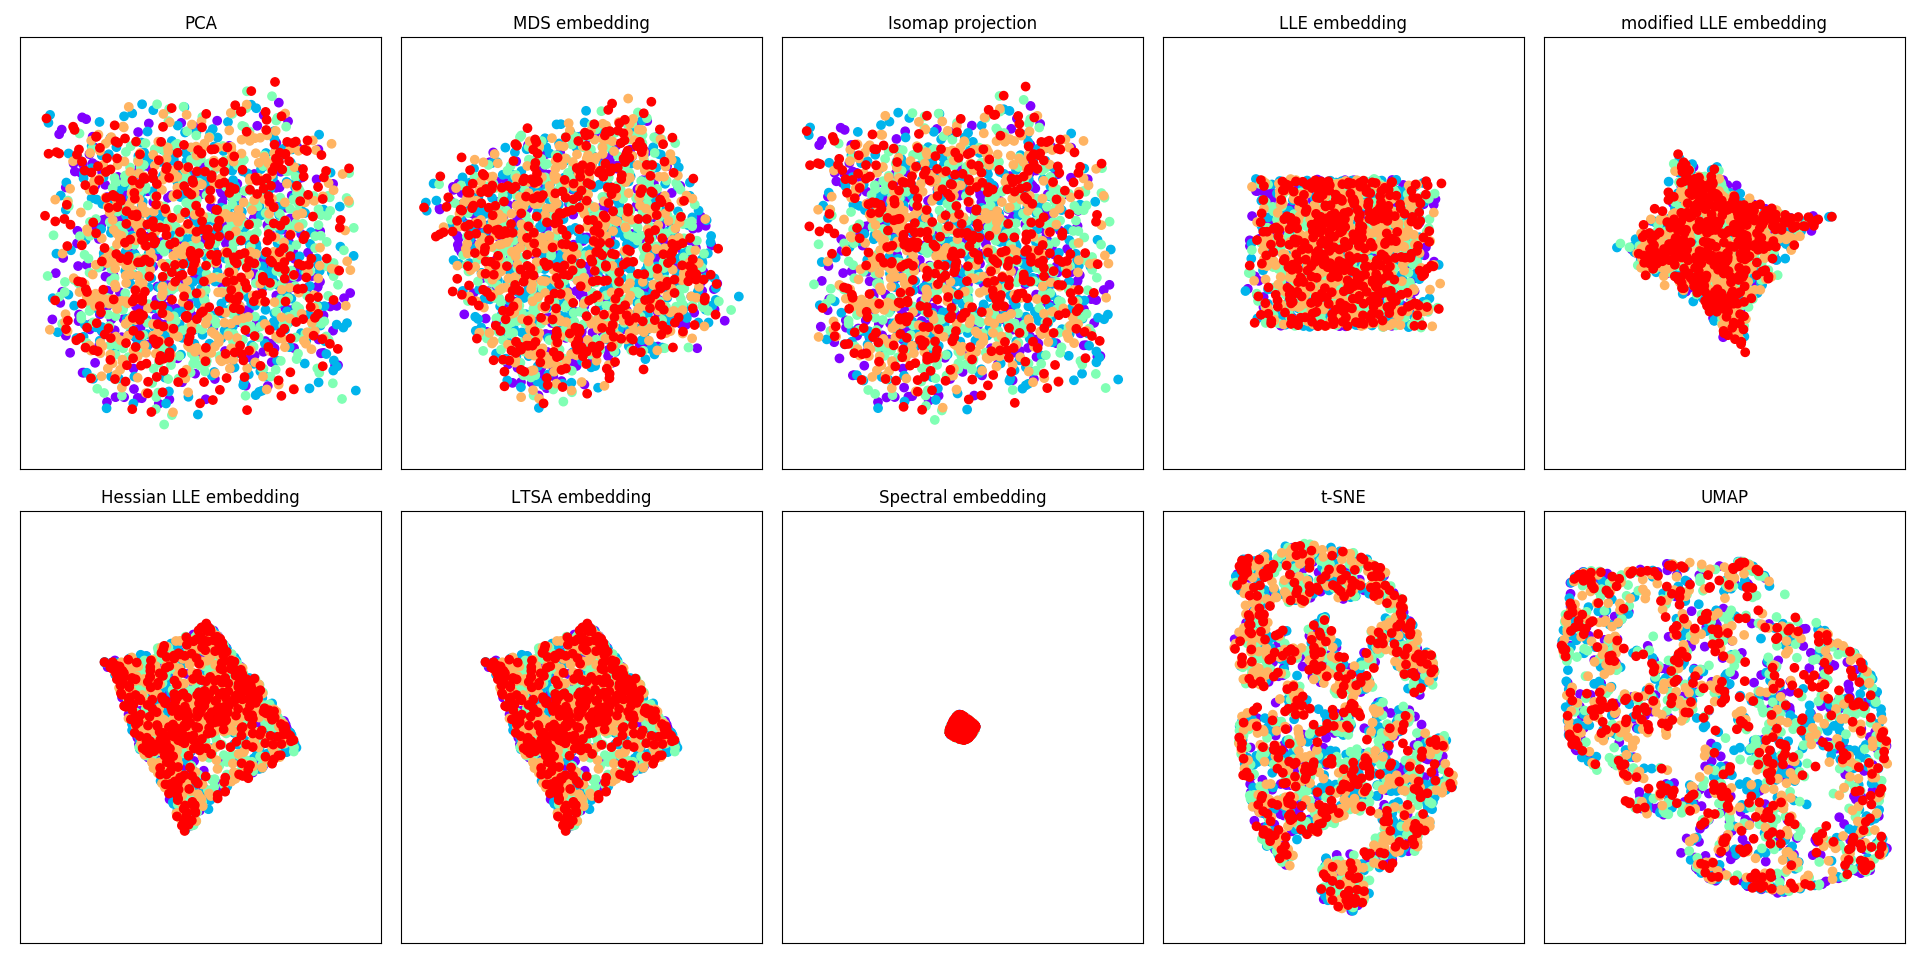
\includegraphics[width=\textwidth]{resources/images/reduction/compare/xr.png}
    \caption{Prikaz rezultata algoritama za učenje mnogostrukosti na primjernu slučajno generiranih podataka}
    \label{fig:xr}
\end{figure}

Iz rezultata, moguće je vidjeti kako većina algoritama ne unosi mnogo pristranosti. Algoritam spektralnog ugrađivanja svrstao je podatke u jednu grupu, ali zato algoritmi t-SNE i UMAP, usprkos nepostojećoj temeljnoj strukturi forsiraju stvaranje grupa. Dodatno, valja naglasiti da je ovaj problem više istaknut kod t-SNE algoritma.

\paragraph{Skup podataka "Fashion MNIST"}

Fashion MNIST je skup podataka odjevnih predmeta kompanije Zalando, a dostupan je na github.com/zalandoresearch/fashion-mnist. Sastoji od skupa za učenje koji sadrži 60000 primjera i od skupa za testiranje koji sadrži dodatnih 10000 primjera. Svaki primjer je crno-bijela slika odjevnog artikla veličine 28x28 (dakle ima 784 značajke) grupirane u 10 razreda. Primjeri slika kakve nalazimo u ovom skupu podataka mogu se vidjeti na slici \ref{fig:fmnist} Ideja Fashion MNIST skupa podataka je da bude direktna zamjena za MNIST; set rukom pisanih znamenaka koji je vrlo popularan u svijetu strojnog učenja. Iz tog razloga skup Fashion MNIST dizajniran je da ima jednaku veličinu slika i strukturu skupova za učenje i testiranje kao i MNIST.

\begin{figure}[htb]
    \centering
    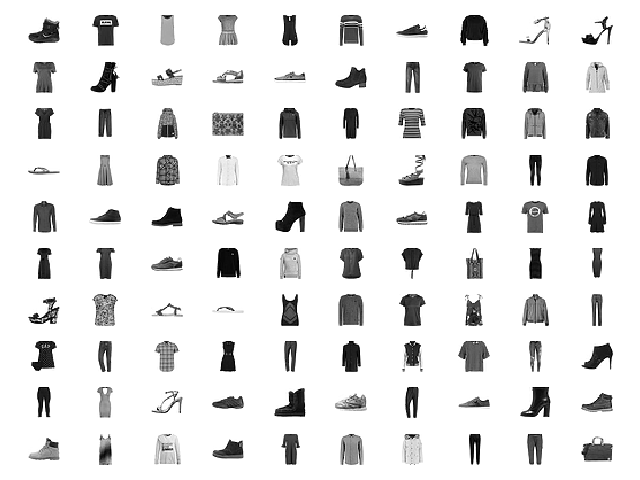
\includegraphics[width=11cm]{resources/images/reduction/compare/fmnist.png}
    \caption{Dio skupa podataka Fashion MNIST}
    \label{fig:fmnist}
\end{figure}

S obzirom na postojanje mnogih primjera korištenja algoritama za redukciju dimenzionalnosti na MNIST skupu podataka, jedan od kojih je \cite{scikit-learn} u ovom radu odlučeno je pokazati kako ovi algoritmi funkcioniraju na zahtjevnijem setu podataka kao što je Fashion MNIST koji predstavlja problem koji je bliži onima iz stvarnog svijeta.

\begin{figure}[htb]
    \centering
    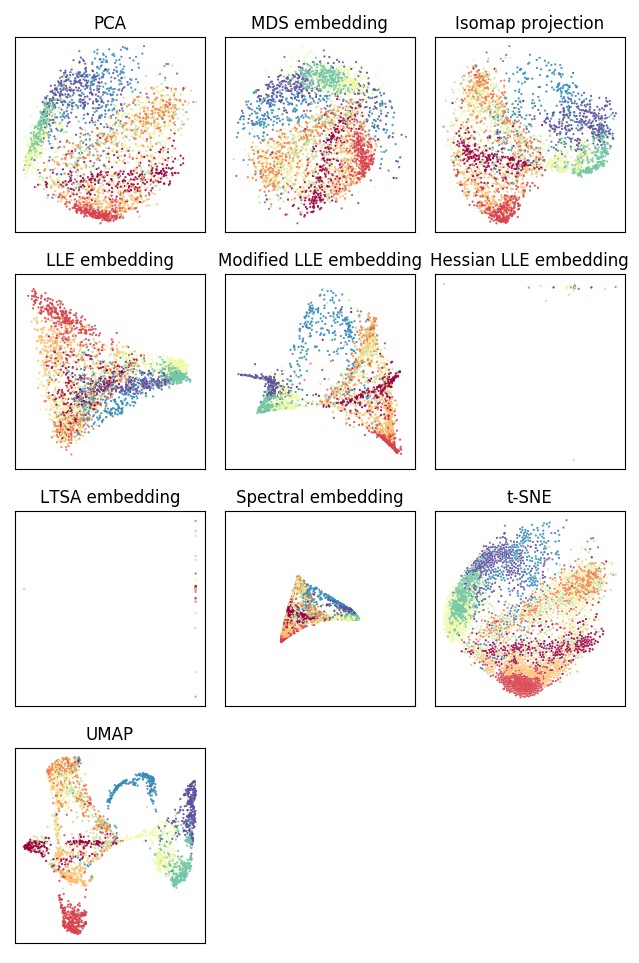
\includegraphics[width=\textwidth]{resources/images/reduction/compare/xfmnist.png}
    \caption{Rezultati algoritama na skupu Fashion MNIST}
    \label{fig:xfmnist}
\end{figure}

Na slici \ref{fig:xfmnist} vidljivi su vrlo zanimljivi rezultati koji pokazuju ponašanje na primjeru sličnijem stvarnim podacima. Cijelo vrijeme tijekom evaluiranja rezultata bitno je na umu imati kako je izvedena redukcija dimenzionalnosti generirala iznimno niskodimenzionalnu mnogostrukost od samo dvije dimenzije. Ovo je prvenstveno zbog ograničenja mogućnosti vizualiziranja viših dimenzija kvalitetno. No, uzevši to u obzir, ideja ovog primjera je pokazati neka od svojstva ovih algoritama.

Iz ovog se primjera može vidjeti iako na jednostavnim primjerima algoritmi rade vrlo dobro, u stvarnosti situacija je puno komplicirana. PCA algoritam, iako naravno ne savršen, pokazuje zanimljive rezultate vrlo slične onima od kompliciranijim algoritmima kao što su MDS u vremenu koje je nekoliko magnituda manje od svih ostalih algoritama. U rezultantnim mnogostrukostima tih algoritama možemo vidjeti odvajanje razreda do neke mjere, ali neki razredi koji su prostorno sličniji drugima su se pomiješali. Marginalno bolji rezultat dobiven je Isomap projekcijom. Algoritmi HLLE i LTSA, očekivano, dijele vrlo slične rezultate, oba koja su nažalost neuporabljiva. Naravno to ne znači da su ovi algoritmi loši, daleko od toga, to samo znači da na ovom konkretnom primjeru (podacima i rezultantnoj dimenziji) oni nisu uspješno mogli odrediti ugrađenu mnogostrukost. Ignorirajući njih, LLE i algoritam spektralnog ugrađivanja rezultirali su najlošijom vizualizacijom te je miješanje grupa kod njih najizraženije. Nedostatke LLE algoritama kod ovog primjera popravio je algoritam MLLE kod kojeg se grupiranje može jasno vidjeti. Algoritam t-SNE, koji je od svog izlaza bio standard za ovakvu primjenu, definitivno je rezultirao vizualizacijom koja je lošija od očekivanog. Naravno ukoliko bi se parametar \emph{preplexity} povećao sa 100 na 200 rezultanta slika bi pokazivala bolje grupiranje ali bi ujedno unijelo ogroman vremenski trošak na već ovako zahtjevan algoritam. Uz to, t-SNE pokazuje svojstva grupiranja bolja nego prijašnji algoritmi. Zadnji, ali ne manje važan, algoritam UMAP dao je objektivno najbolje rezultate, s jasnim granicama većine grupa, u vremenu koje je kraće od svih nelinearnih algoritama testiranih u ovom radu.

\bigskip
\begin{tikzpicture}
    \label{graph:timings}
    \begin{axis}[
            title  = Trajanje izvođenja algoritama na skupu Fashion MNIST,
            xbar, xmin=0, xmax=50,
            symbolic y coords = {UMAP, t-SNE, Spectral, LTSA, HLLE, MLLE, LLE, Isomap, MDS, PCA},
            ytick=data,
            ylabel={Algoritam},
            xlabel={vrijeme izvršavanja, s},
            axis y line*=none,
            axis x line*=bottom,
            nodes near coords,
            nodes near coords align={horizontal},
            width=.7\textwidth,
        ]
        \addplot coordinates {
                (0.12,PCA)
                (30.24,MDS)
                (29.41,Isomap)
                (24.04,LLE)
                (27.59,MLLE)
                (34.41,HLLE)
                (38.78,LTSA)
                (18.69,Spectral)
                (38.30,t-SNE)
                (12.29,UMAP)
            };
        % \legend{Topics, Posts}
    \end{axis}
\end{tikzpicture}

\chapter{Primjena redukcije dimenzionalnosti u SCA}

Kao što je spomenuto u uvodu, ovaj rad je temeljen na radu od \cite{8836108} u kojem se autori koncentriraju na utjecaj tehnika odabira značajki \engl{feature selection} u analizi koja koristi sporedna sredstva. Točnije, cilj je odrediti kako efikasnost SCA može biti povećana korištenjem tehnike odabira značajki. Dodatno u radu je istražena i metoda PCA kako bi se dao uvid u razlike odabira značajki i redukcije dimenzionalnosti. Iz spomenutog rada preuzete su notacije i skupovi podataka korišteni za evaluaciju metoda. U ovom poglavlju bit će opisana i raspravljena primjena redukcije dimenzionalnosti u analizi koja koristi sporedna sredstva uređaja. Radi boljeg razumijevanja dodatno će se opisati bitniji koncepti korišteni prilikom metode prezentirane u radu koji nisu obuhvaćeni prijašnjim poglavljima. Zatim će biti opisana metoda kojom su dobiveni rezultati, a posljednjem odjeljku ovog poglavlju ti dobiveni rezultati bit će izneseni, vizualizirani i diskutirani.

\section{Pozadina}

\subsection{AES kriptografski algoritam}
Američki nacionalni institut standarda i tehnologije \engl{National Institute of Standards and Technology, NIST} je u razdoblju od 1997. do 2000. godine raspisao natječaj s ciljem pronalaska novog standarda u kriptografiji koji bi naslijedio DES. Taj novi standard bi se zvao napredni enkripcijski standard \engl{Advanced Encryption Standard, AES}. Od mnoštva kandidata petnaest je odabrano u uži krug, a od njih zatim pet finalista: Rijndael, Serpent, MARS, Twofish, RC6. Iako su svi finalisti imali jednaku jačinu sigurnosti, NIST je odabrao algoritam Rijndael kao novi standard zbog dobrih performansi na većini platformi te jednostavnosti implementacije. Rijndael je simetrični blokovski kriptoalgoritam koji su razvili dvojica belgijskih kriptografa Joan Daemen i Vincent Rijmen, po kojima je i imenovan. Rijndael može biti specificiran s veličinom bloka i ključa koja je višekratnik od 32 bita između 128 bita i 256 bita. S druge strane, AES ima fiksnu veličinu bloka od 128 bita i veličinu ključa od 128, 192 i 256 bita. AES je dakle podskup Rijndael algoritma. Broj krugova $T$ u AES-u ovisi o veličini ključa te za verzije AES-128, AES-129 i AES-256 je 10, 12 i 14 respektivno. AES koristi četiri operacije $SubBytes$, $ShiftRows$, $MixColumns$ i $AddRoundKey$. Funkciju jednog kruga, $R_i, 1 \le i \le T$ definiramo kao
\begin{equation}
    R_i =
    \begin{cases}
        AddRoundKey_i \circ MixColumns \circ ShiftRows \circ SubBytes & , i < T \\
        AddRoundKey_i \circ ShiftRows \circ SubBytes                  & , i = T
    \end{cases}
\end{equation}
Prije prvog kruga, u koraku $AddRoundKey_0$ koristi se izbijeljeni ključ tako da se enkripcija sa $T$ krugova i ključem $K$ opisuje kao
\begin{equation}
    E_k = R_T \circ \dots \circ R_1 \circ AddRoundKey_0.
\end{equation}
Sve četiri operacije izvode se na 128 bitnom bloku raspoređenom u $4 \times 4$ matricu
\[
    \begin{pmatrix}
        b_{0} & b_{4} & b_{8}  & b_{12} \\
        b_{1} & b_{5} & b_{9}  & b_{13} \\
        b_{2} & b_{6} & b_{10} & b_{14} \\
        b_{3} & b_{7} & b_{11} & b_{15}
    \end{pmatrix}
\]
i na Rijndael konačnom polju $\mathbb{F}_{256}$.

\paragraph{Operacija $SubBytes$:} U ovoj operaciji svaki od 16 bajtova u matrici je zamijenjen s drugom vrijednošću prema tablici koja se naziva supstitucijska kutija (\englnp{Substitution box}, dalje \emph{S-Box}). Ova tablica je javna, a dizajnirana je tako da nije moguće da se vrijednost mapira sama u sebe te nije moguće da se svi bitovi preokrenu.

\paragraph{Operacija $ShiftRows$:} Ova operacija je vrlo jednostavna, te sve što radi je za $i$-ti red tablice, gdje za i vrijedi $0 \le i \le 3$, cirkularno rotira vrijednosti lijevo za $i$ pozicija.

\paragraph{Operacija $MixColumns$:} Ova operacija nastavlja se na prošlu, te se u njoj sada miješaju stupci. Ovaj korak se izvodi pomoću matričnog množenja. Dakle svaki stupac, kao vektor se množi s tablicom M
\[
    M =
    \begin{pmatrix}
        2 & 3 & 1 & 1 \\
        1 & 2 & 3 & 1 \\
        1 & 1 & 2 & 3 \\
        3 & 1 & 1 & 2 \\
    \end{pmatrix}
\]
Prilikom dekripcije koristi se inverz matrice $M^{-1}$.

\paragraph{Operacija $AddRoundKey$:} Konačno, u ovoj se operaciji našoj matrici dodaje ključ trenutnog kruga $K_i$ koristeći isključivo-ILI operaciju.

\subsection{Slučajna šuma}

Slučajna šuma (\englnp{Random forest}, skrać \emph{RF}) vrlo su poznat stohastički ansambl osnovnih klasifikatora po imenu stablo odluke.

\paragraph{Stabla odluke}
su neparametarska, diskriminativna metoda aproksimacije funkcije diskretnih vrijednosti koja može učiti disjunktivne koncepte i robusna je na šum. Stablo odluke koristi vrlo intuitivan koncept a sastoji se od čvorova koja predstavljaju pitanja a grane čvorova predstavljaju odgovore na ta pitanja. Listovi stabla su konačni razredi. Dakle na nekom čvoru se "odgovara na pitanje" a odgovor na to pitanje zatim vodi grananjem na neko drugo pitanje. Odabir atributa koji će činiti čvorove određuju se koristeći informacijsku dobit, koja je usko vezana s entropijom. Korijeni stabla su atributi s najvećom informacijskom dobiti.
\begin{definition}
    Za neku diskretnu slučajnu varijablu $X$ s mogućim skupom vrijednosti $\{x_1, \dots, x_n\}$ i funkciju vjerojatnosti $P$ definiramo entropiju kao:
    \begin{equation}
        H(X) = - \sum_{i=1}^n P(x_i) \log_b P(x_i)
    \end{equation}
    \label{def:entropy}
\end{definition}

\begin{definition}
    Neka je  $\bm{D} = \left\{ (\bm{x}^{(i)}, y^{(i)}) \right\}_{i=1}^N$ skup označenih primjera, gdje je $x_a \in \mathcal{V}(a)$ je vrijednost $a$-tog atributa primjera $\bm{x}^{(i)}$, a $y$ oznaka odgovarajućeg razreda. $H$ je entropija definirana u definiciji  \ref{def:entropy}. Za vrijednost $v$ i atribut $a$ neka
    \begin{equation}
        S_a(v) = \left\{ \bm{x} \in \bm{D} \vert x_a = v \right\}
    \end{equation}
    bude definiran kao podskup od $\bm{D}$ za koji atribut $a$ jednak vrijednosti $v$. Tada informacijsku dobit \engl{gain} skupa $\bm{D}$ za atribut $a$ definiramo kao
    \begin{equation}
        IG(\bm{D}, a) = H(D) - \sum_{v\in \mathcal{V}(a)}
        \frac{\vert S_a(v) \vert}{\vert \bm{D} \vert} H(S_a(v))
    \end{equation}
\end{definition}


Slučajne šume sastoje se od mnoštva ovakvih stabla odluke, svako od kojih daje zasebnu klasifikaciju, a zatim razred s najviše "glasova" postane rezultantan razred RF modela. Kako bi se osnovni klasifikatori maksimalno nadopunjavali, potrebno je da imaju vrlo malu međusobnu korelaciju. Kako bi se to postiglo, iskorištava se svojstvo stabla odluke da budu vrlo osjetljivi na podatke na kojima su trenirani, tako da svako stablo slučajno iz skupa podataka uzorkuje s ponavljanjem. Ovaj postupak naziva se bootstrap agregiranje \engl{Bagging}. Vremenska kompleksnost učenja ovog algoritma je $O(I \cdot k \cdot N \cdot \log N)$ gdje je $I$ broj stabala u slučajnoj šumi, $k$ je broj atributa koji se razmatra u svakom čvoru stabla, a $N$ je broj uzoraka.

\subsection{Entropija pogađanja}

Entropija pogađanja (\englnp{Guessing Entropy}, dalje. \emph{GE}), koju je originalno definirao \cite{massey1994guessing}, predložena za korištenje u analizi koja koristi sporedna sredstva od \cite{kopf2007information}. Ova mjera jednostavno predstavlja težinu da napadač pogodi vrijednost slučajne varijable. Točnije GE neke slučajne varijable $X$ je prosječan broj pitanja tipa "vrijedili da je $X = x$" koja moraju biti postavljena da bi se točno odredila vrijednost $X$. Ako pretpostavimo da su vjerojatnosti $p$ poznate, optimalna procedura je pokušati sve vrijednosti $x$ prema opadajućem redoslijedu njihovih vjerojatnosti. Generalnije, neka je $\mathcal{X}$ indeksiran tako da uvijek vrijedi $p_x(x_i) \ge p_x(x_j) \iff i \le j$. Tada se entropija pogađanja od $X$, $G(X)$, definira kao
\begin{equation}
    G(X) = \sum_{1 \le i \le \vert \mathcal{X}} i p_x(x_i)
\end{equation}
A analogno uvjetnoj entropiji, uvjetna entropija pogađanja definira se kao
\begin{equation}
    G(X \vert Y) = \sum_{y \in \mathcal{Y}} p_y(y) G(X \vert Y = y)
\end{equation}
koja predstavlja broj pogađanja potrebnih za određivanje vrijednosti X kada je vrijednost Y poznata. Dakle možemo povezati entropiju pogađanja s pojmom dobrobiti koji se koristi u kontekstu višestruke linearne kriptoanalize kao mjera koliko je kompleksnost iscrpnog pretraživanja smanjenja zahvaljujući napadu \citep{standaert2009unified}.

\section{Skupovi podataka}
U ovom radu, korištena su tri skupa podataka, koja predstavljaju razne težine situacija koje se često mogu dogoditi. Prvi, najjednostavniji, skup podataka sadrži podatke koji ne implementiraju protumjere te sadrže vrlo malo šuma. Drugi, malo realniji, primjer je skup podataka koji kao ni prvi nema implementirane protumjere ali zato ima mnogo šuma u podacima. Ovakva situacija češća je u stvarnosti zbog nemogućnosti izvođenja savršenih mjerenja sporednih sredstava. Konačno, posljednji skup podataka koji je korišten u ovom radi, implementira protumjere u obliku slučajnih kašnjenja.

\subsubsection{DPAcontest v4}
U ovom skupu podataka sadržana su mjerenja maskirane programske AES implementacije. Kako je maska poznata, lagano je pretvoriti ove podatke u skup bez protumjera. Pošto je ovo programska implementacija, većina odljeva informacija događa se za vrijeme izvođenja zamjene pomoću kutija za zamjene (\englnp{Substitution box}, dalje \emph{S-Box}), a ne za vrijeme zapisivanja podataka u registre. Zbog toga se napad izvodi u prvom krugu, a model odljeva je definiran kao
\begin{equation}
    Y(k*) = \aessbox{}\left[ P_{b_1} \oplus k* \right] \oplus \underbrace{M}_\text{poznata maska},
\end{equation}
gdje je $p_{b_1}$ $b_1$-ti oktet originalne poruke. U ovom radu napada se prvi samo prvi oktet, dakle $b_1 = 1$.


\subsubsection{AES\_HD} Ovaj skup podataka reprezentira nezaštićenu implementaciju AES-128 koja je napisana u VHDL-u. Za eksternu komunikaciju koristi se UART modul. Za implementaciju korišten je Xilinx Virtex-5 FPGA na SESEBO GII evaluacijskoj ploči. Sporedna sredstva mjerena su usko-poljnom elektromagnetskom sondom visoke osjetljivosti na kondenzatoru za odvajanje smještenom na krugu napajanja. Mjerenja su uzorkovana na Teledyne LeCroy Waverunner 610zi osciloskopu. Ukupni obujam dizajna je 1850 tablica traženja \engl{lookup tables} i 742 bistabila. U ovom slučaju napad se radi na posljednji krug AES-a tako da je prikladan i često korišten model odljeva onaj koji opisuje zapisivanje podataka u registre prilikom zadnjeg kruga, tj.
\begin{equation}
    Y(k*) = HW(\underbrace{\aessbox^{-1} \left[ C_{b_1} \oplus k* \right]}_\text{prošla vrijednost registra} \oplus \underbrace{C_{b_2}}_\text{oktet kriptirane poruke}),
\end{equation}

\subsubsection{Random delay}
Posljednji slučaj je stvarna zaštićena programska implementacija AES-a izvedena na 8 bitnom Atmel AVR mikrokontroleru. Implementirana zaštita je u obliku slučajnih kašnjenja. Napad se kao i u prvom skupu podataka izvodi na prvu $\aessbox$ operaciju.

\section{Metoda}

Za sve korištene skupove podataka, opisane u odlomku prije, primijenjena su dva različita modela odljeva. Osnovniji koristeći direktno međuvrijednosti tragova i drugi koji koristi Hammingovu težinu $HW$. Ti modeli su označeni kao "value" i "HW" respektivno. Broj značajki $D$ za svaki primjer odabran je da bude 50. Iz inicijalnog skupa podataka napravljena su dva podskupa: podskup podataka $\bm{D}_{train}$ za učenje koji sadrži 10 000 tragova (primjera) i podskup za testiranje $\bm{D}_{test}$ koji sadrži 25 000 tragova (primjera). Valja napomenuti da vrijedi $\bm{D}_{train} \cap \bm{D}_{train} = \emptyset$. Cilj je za skup podataka dimenzije $D$ redukcijom dimenzionalnosti pronaći skup podataka dimenzije $D_m$ gdje vrijedi da je $D_m < D$.
Metode redukcije dimenzionalnosti koje se koriste su one opisane u prošlim poglavljima\footnote{Algoritmi MDS i t-SNE nisu korišteni u ovom djelu rada zbog nemogućnosti generalizacije na neviđenim primjerima}. Za većinu metoda potrebno je odrediti broj susjeda $N_n$ koji algoritam koristi prilikom redukcije. Eksperimentalno izabrane kombinacije parametara korištene $D_m$ i $N_n$ korištene u ovom radu uz notaciju
\[(D_m, A) = \{(D_m, N_n) | N_n \in A\}, \quad D_m \in \mathbb{N}, A \subseteq \mathbb{N} \]
mogu biti opisane kao
\begin{align*}
    S = \{
     & (3, \{10\}) \cup
    (7, \{10, 20, 40\}) \cup
    (10, \{10, 30, 70\}) \cup
    (15, \{10, 50, 70, 150\}) \cup     \\
     & \quad(25, \{10, 50, 400\}) \cup
    (40, \{50, 500, 1000\})
    \}
\end{align*} Za neke algoritme, neke kombinacije navedenih parametara nisu moguće te su one zanemarene. Dodatno je korištena trivijalna metoda definirana funkcijom identiteta $f(x) = x, \forall x$. Takav transformator koristi se kao referentna vrijednost, a označen je sa pseudonimom "dummy". Uz osnovne metode redukcije dimenzionalnosti dodana je i hibridna metoda koja koristi rijetke slučajne projekcije \engl{Sparse Random Projection, SRP}. Za korištene skupove podataka pokazalo se da rijetke slučajne projekcije za redukciju u dimenziju 30 zadržavaju razumnu količinu informacija originalnog prostora dok istovremeno pružaju poželjnu razinu redukcije. Iz tog razloga hibridne metode prvo koristeći metodu SRP reduciraju dimenzionalnost u dimenziju 30, a zatim korištenjem neke osnovnih metoda redukcije dimenzionalnosti se prostor dodatno smanjuje u dimenziju $D_m$ za koju vrijedi $D_m < 30$. Takve hibridne metode notirane su koristeći prefix "srp30+" uz naziv osnovne metode redukcije korištene. Dakle ako bismo, primjerice, za hibridnu metodu koristili metodu SRP u kombinaciji s metodom LLE tada ona bila notirana kao "srp30+lle".

Nakon transformacije, skup podataka koji sada ima dimenziju $D_m$ postavlja se kao ulaz klasifikatora. Klasifikator korišten u ovom radu je opisana metoda slučajnih šuma koji je odabran zbog otpornosti na šum što je u ovom radu od velike važnosti. Radi usporedbe metoda za redukciju dimenzionalnosti broj stabala korištenih u ovom koraku je fiksno postavljen na 100. Naravno za određenu metodu i njene parametre moguće je pronaći optimalne parametre prilikom klasifikacije. Ako koristimo model odljeva s međuvrijednosti(value) broj razreda je 256 te predstavlja dekadsku vrijednost okteta koji pokušavamo odrediti, dok ako je riječ o metodi s Hammingovom težinom tada je broj razreda 9 i on naravno odgovara Hammingovoj težini okteta. Kao mjeru performansi, koristi se točnost klasifikatora, no uz to, zbog činjenice da ta mjera često ne pokazuje stvarnu situaciju, dodatno se koristi stopa uspjeha \engl{success rate} i entropija pogađanja.

\section{Rezultati}

U tablicama \ref{tab:dpa_hw}-\ref{tab:rd_value} prezentirane su vrijednosti točnosti klasifikatora i minimalna dobivena vrijednost entropije pogađanja $GE_{min}$, a na slikama \ref{fig:dpa_hw}-\ref{fig:rd_value} prikazane su vrijednosti entropije pogađanja ovisne o broju tragova. Zbog prostornih ograničenja, prikazani podaci predstavljaju reprezentativni podskup testiranih scenarija. Rezultati svih izvedenih testiranja dostupni su na https://github.com/eugen-vusak/manifold-SCA/blob/master/practical/reports/summary.xlsx. Za tablice \ref{tab:dpa_hw}-\ref{tab:rd_value} uzete su vrijednosti deset najboljih metoda ne uključujući metodu "dummy", koja je zatim dodana zasebno. Na isti način, za slike \ref{fig:dpa_hw}-\ref{fig:rd_value} su odabrane tri najbolje vrijednosti (bez  metode "dummy"), i dodatno referentna metoda "dummy". Na navedenim slikama isprekidanom sivom linijom označena je granica za koju smatramo da je napad bio uspješan, a metode su u legendi opisane oblikom "$\text{ime\_metode}(D_m, N_n)$", iako ako metoda ne koristi neke parametre oni su izostavljeni i iz naziva.

\subsection{DPAcontest v4}
Tablice \ref{tab:dpa_hw} i \ref{fig:dpa_value} pokazuju rezultate za skup podataka DPAcontest v4 dobivene za modele odljeva HW i value. Za HW model na tablici \ref{tab:dpa_hw} možemo vidjeti kako je najbolja metoda UMAP s vrlo malom redukcijom za samo 10 dimenzija. U kontrastu s time druge dvije najuspješnije metode su hibridne metode obije kod kojih je rezultantna dimenzija 10. Te metode koriste metode LTSA i MLLE kao osnovnu metodu. Metoda LLE pokazala se relativno uspješnom s raznim rasponom parametara. Bitno je naglasiti da su ove metode postigle mnogo bolje rezultate od referentne metode. Za ovaj specifični eksperiment pokazalo se da dimenzija 10 s 30 najbližih susjeda globalno pokazuje najbolje rezultate. Također vidljivo je da visoka točnost ne rezultira nužno dobrim rezultatima u kontekstu entropije pogađanja. Na slici \ref{fig:dpa_hw} vidljivo je da je razlika između prve tri metode relativno velika, te da ovisno o metodi broj potrebnih tragova može odstupati za približno 40.

Rezultati za value odljev, vidljivi na tablici \ref{tab:dpa_value} prikazuju drugačiju sliku. U ovom slučaju dvije najbolje metode obije izvode redukciju u prostor od 25 dimenzija. I u ovom slučaju metoda UMAP pokazala se najuspješnijom ali u ovom slučaju to je s većom redukcijom. Dodatno metoda srp30+UMAP pokazala se vrlo uspješnom, marginalno lošijom od metode MLLE.  Slika \ref{fig:dpa_value} pokazuje kako je razlika između najboljih metoda puno manja nego u HW modelu.


\begin{figure}[htb]
    \begin{floatrow}
        \CenterFloatBoxes
        \ffigbox[\FBwidth][]{%
            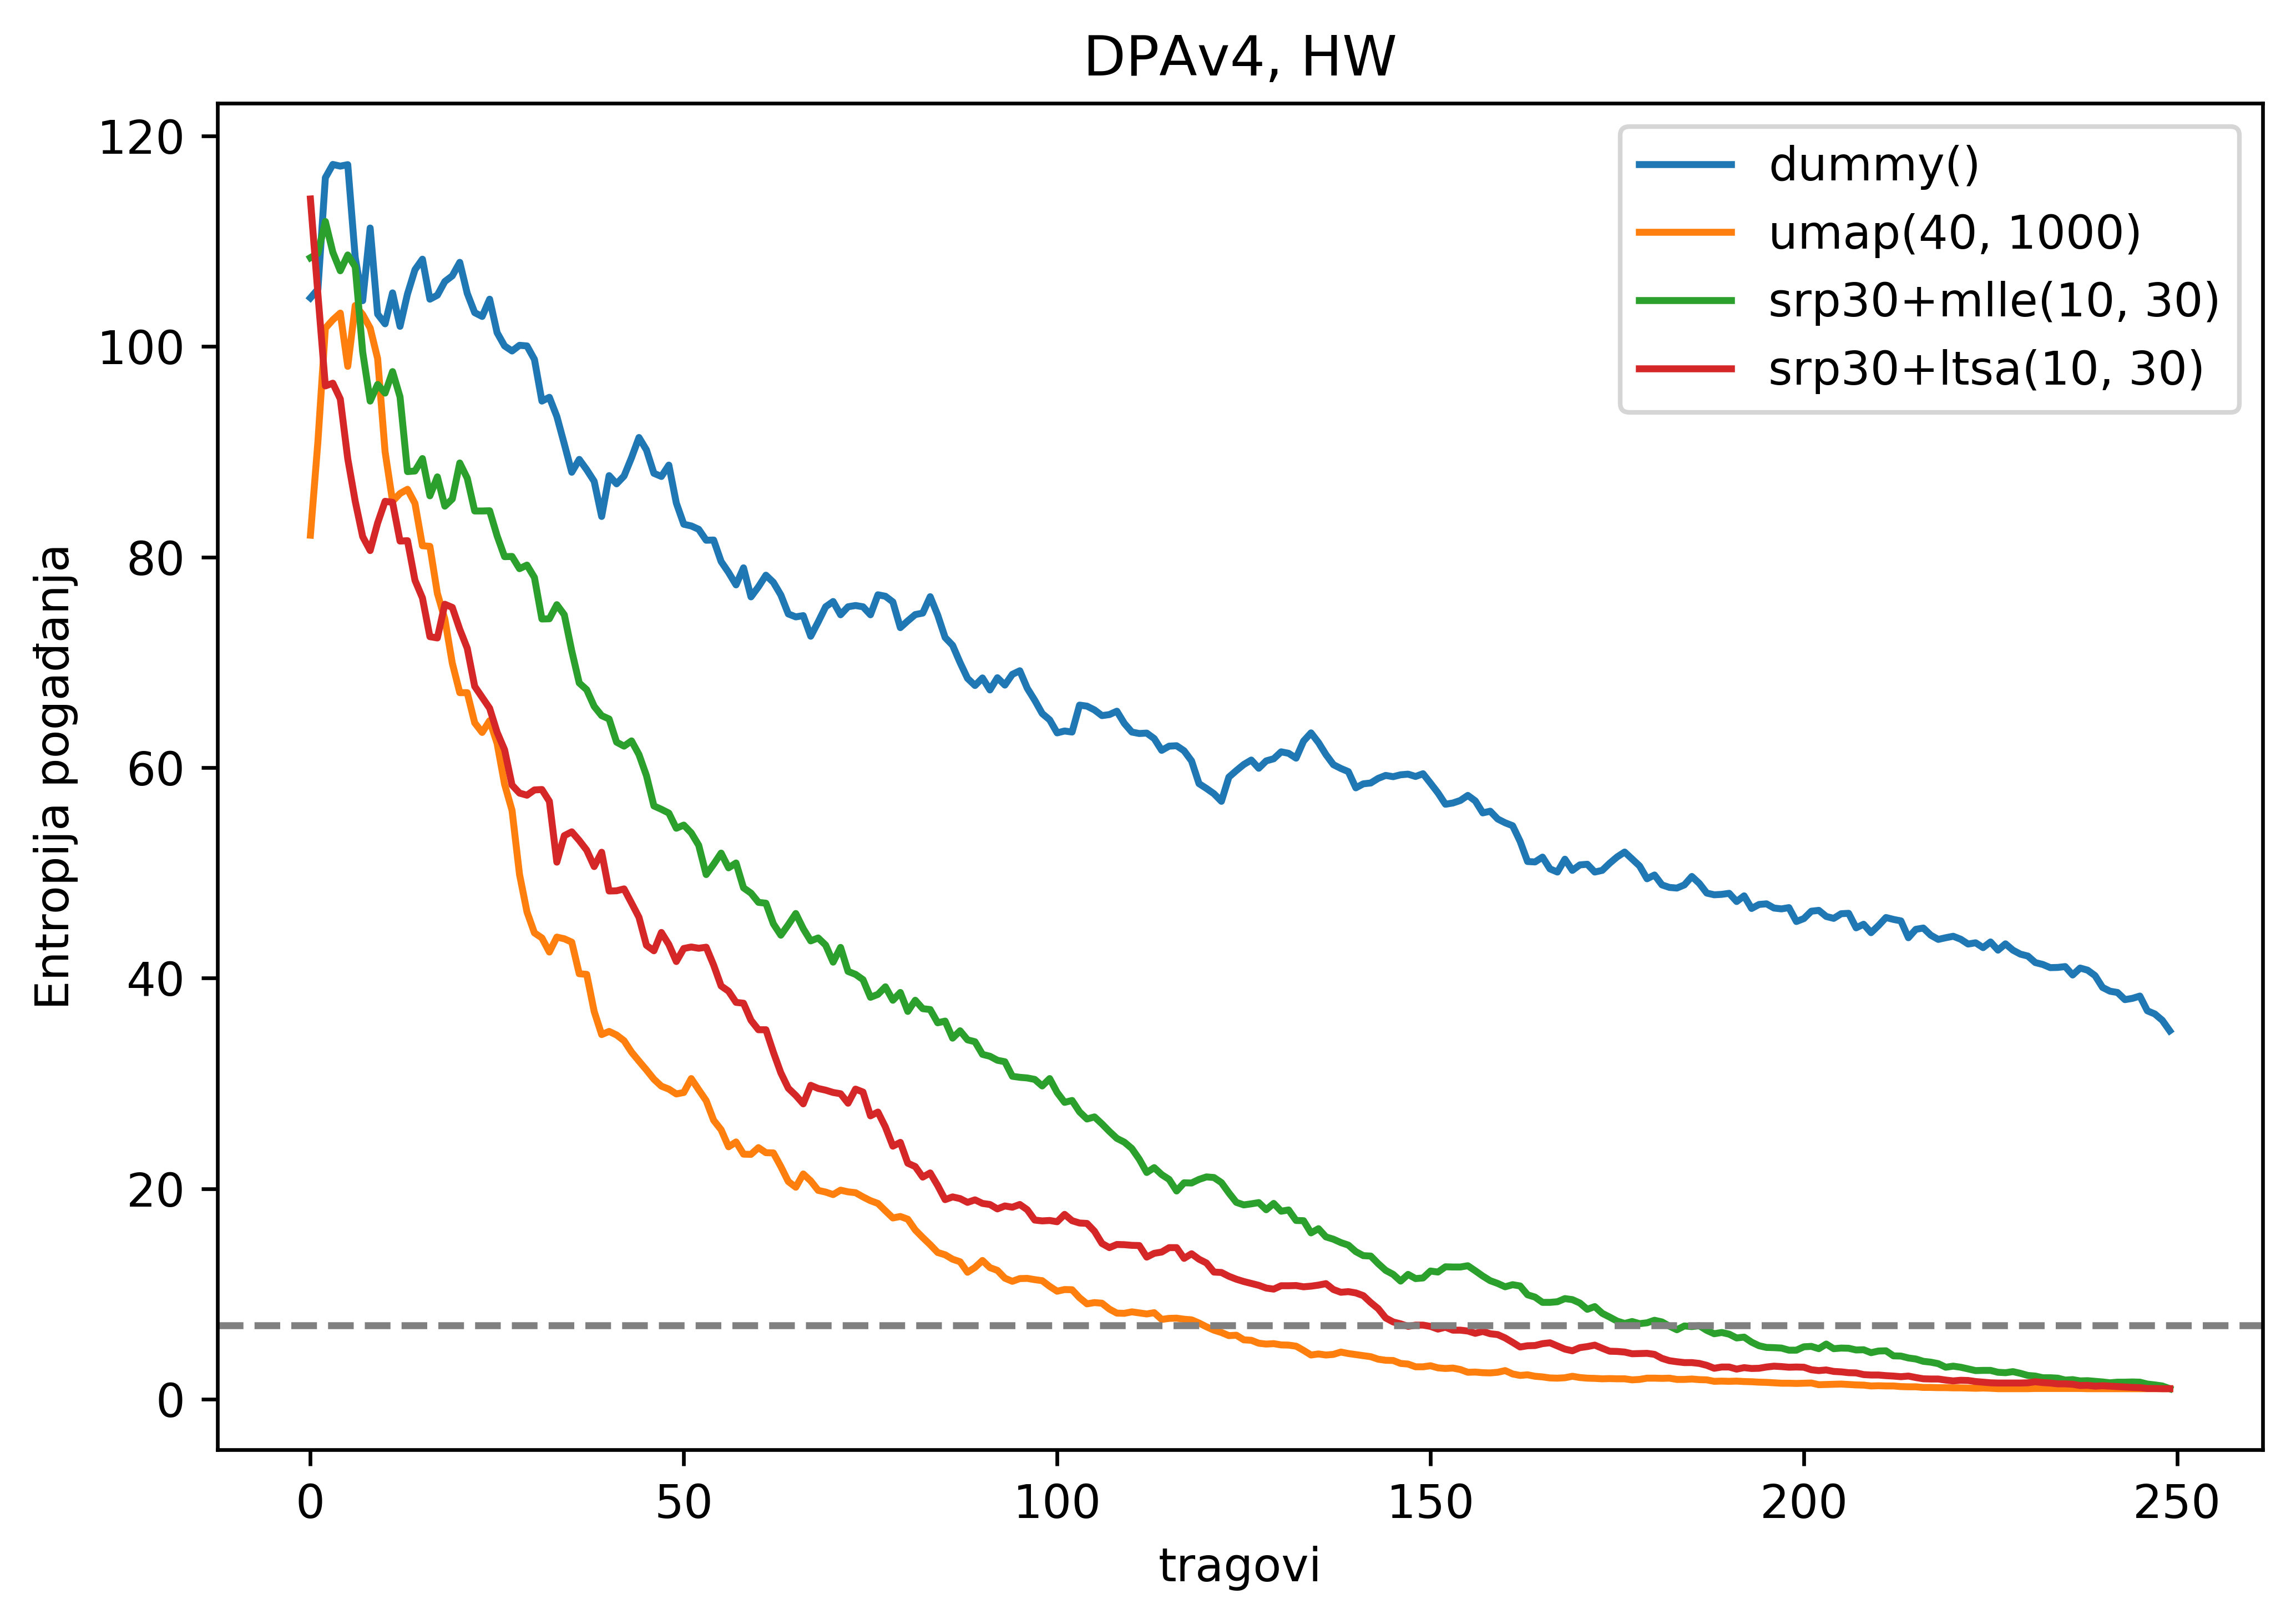
\includegraphics[width=.62\textwidth]{resources/images/application/DPAv4_HW.png}
        }{%
            \caption{GE za skup DPAcontest v4 - model HW}%
            \label{fig:dpa_hw}
        }
        \ttabbox[\FBwidth][]{%
            \resizebox{.32\textwidth}{!}{%
                \setlength\tabcolsep{1.5pt} % default value: 6pt
                \begin{tabular}{lcc|cc}
                    metoda     & $D_m$ & $N_n$ & točnost & $GE_{min}$ \\\hline
                    umap       & 40    & 1000  & 0.74448 & 1          \\
                    srp30+ltsa & 10    & 30    & 0.72476 & 1          \\
                    srp30+mlle & 10    & 30    & 0.79672 & 1          \\
                    lle        & 10    & 30    & 0.73048 & 1.78       \\
                    lle        & 25    & 200   & 0.84988 & 1.86       \\
                    lle        & 20    & 50    & 0.7438  & 2          \\
                    lle        & 25    & 400   & 0.86236 & 2          \\
                    mlle       & 20    & 50    & 0.8826  & 2          \\
                    srp30+mlle & 3     & 10    & 0.71436 & 2          \\
                    lle        & 40    & 500   & 0.83216 & 2.58       \\
                    dummy      &       &       & 0.85656 & 35         \\
                \end{tabular}
            }
        }{%
            \caption{Rezultati za skup DPAcontest v4 - model HW}%
            \label{tab:dpa_hw}
        }
    \end{floatrow}
\end{figure}

\begin{figure}[htb]
    \begin{floatrow}
        \CenterFloatBoxes
        \ffigbox[\FBwidth][]{%
            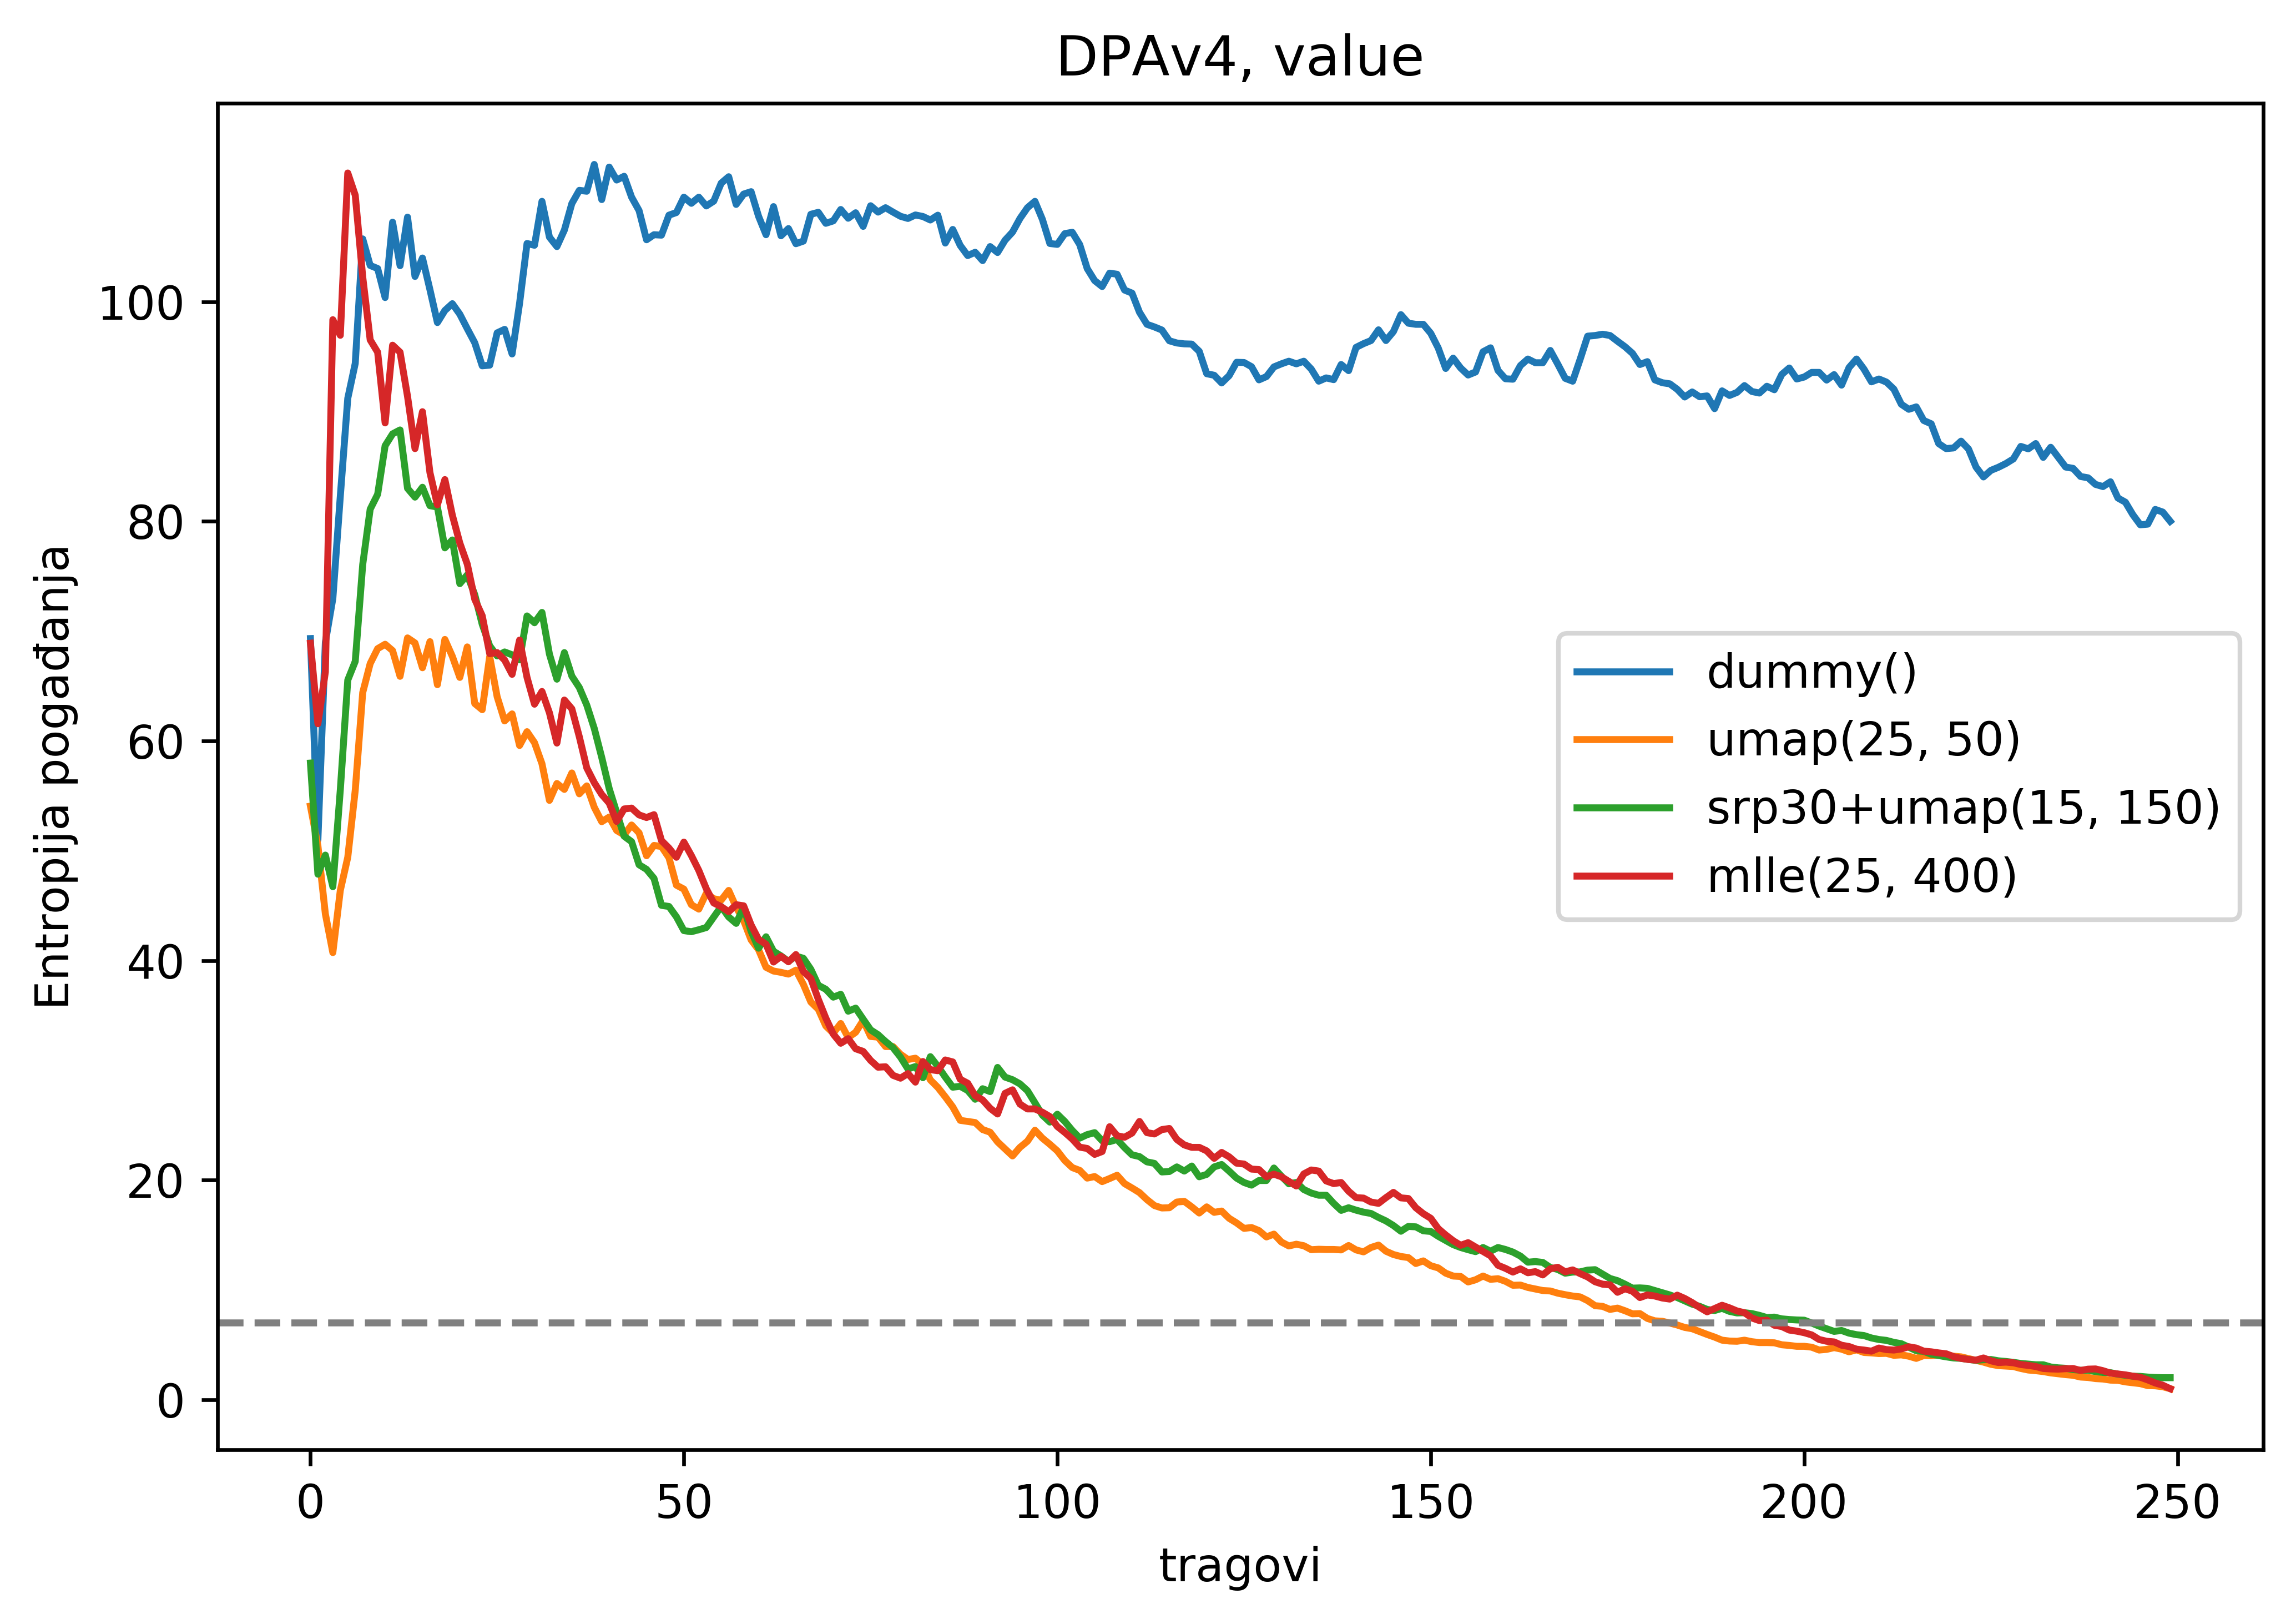
\includegraphics[width=.62\textwidth]{resources/images/application/DPAv4_value.png}
        }{%
            \caption{GE za skup DPAcontest v4 - value model}%
            \label{fig:dpa_value}
        }
        \ttabbox[\FBwidth][]{%
            \resizebox{.32\textwidth}{!}{%
                \setlength\tabcolsep{1.5pt} % default value: 6pt
                \begin{tabular}{lcc|cc}
                    metoda     & $D_m$ & $N_n$ & točnost & $GE_{min}$ \\\hline
                    umap       & 25    & 50    & 0.146   & 1          \\
                    mlle       & 25    & 400   & 0.29872 & 1          \\
                    srp30+umap & 15    & 150   & 0.12028 & 2          \\
                    srp30+hlle & 3     & 10    & 0.00556 & 2          \\
                    ltsa       & 7     & 20    & 0.00464 & 2.88       \\
                    umap       & 40    & 1000  & 0.132   & 2.9        \\
                    lle        & 3     & 10    & 0.12292 & 3          \\
                    lle        & 3     & 10    & 0.1212  & 3          \\
                    mlle       & 10    & 10    & 0.0044  & 3          \\
                    srp30+mlle & 10    & 10    & 0.00444 & 3          \\
                    dummy      &       &       & 0.3466  & 50.98      \\
                \end{tabular}
            }
        }{%
            \caption{Rezultati za skup DPAcontest v4 - value model}%
            \label{tab:dpa_value}
        }
    \end{floatrow}
\end{figure}

\subsection{AES\_HD}
Za skup podataka AES\_HD rezultati su dani u tablicama \ref{tab:aes_hw} za model odljeva HW i za \ref{tab:aes_value} za value model odljeva. Za HW model iako su korištenjem metoda redukcije dimenzionalnosti postignuti bolji rezultati nego kada one nisu implementirane, niti jedna od metoda nije uspješno izvela napad što je vidljivo na slici \ref{fig:aes_value}. Tome je najbliže bila metoda MLLE, dok su sve tri sljedeće metode hibridnog oblika raznih parametara. Manjak odnosa točnosti klasifikatora vrlo je izražena i u ovom primjeru.

Za rezultate na istom skupu podataka, ali koristeći model odljeva value, u rezultatima iz tablice \ref{tab:aes_value} vidljivo kako hibridna metoda koja koristi UMAP, a traženi prostor je vrlo niskodimenzionalan prostor dimenzije 7, je rezultirala najboljim rezultatom. Ista metoda, ali za konačnim prostorom dimenzije 25 je sljedeća. U ovom slučaju generalno se najbolje pokazala redukcija u 7-dimenzionalni prostor. Na slici \ref{fig:aes_value} može se vidjeti nakon koliko tragova su metode smatrane uspješnima. Točnost na ovom skupu podataka vrlo je niska i nalikuje slučajnom pogađanju ($1 / 256$). Za relativno mali broj primjera korišten u skupu za učenje, na ovako teškom skupu s 256 razreda ovakav rezultat nije daleko od očekivanog.
\begin{figure}[htb]
    \begin{floatrow}
        \CenterFloatBoxes
        \ffigbox[\FBwidth][]{%
            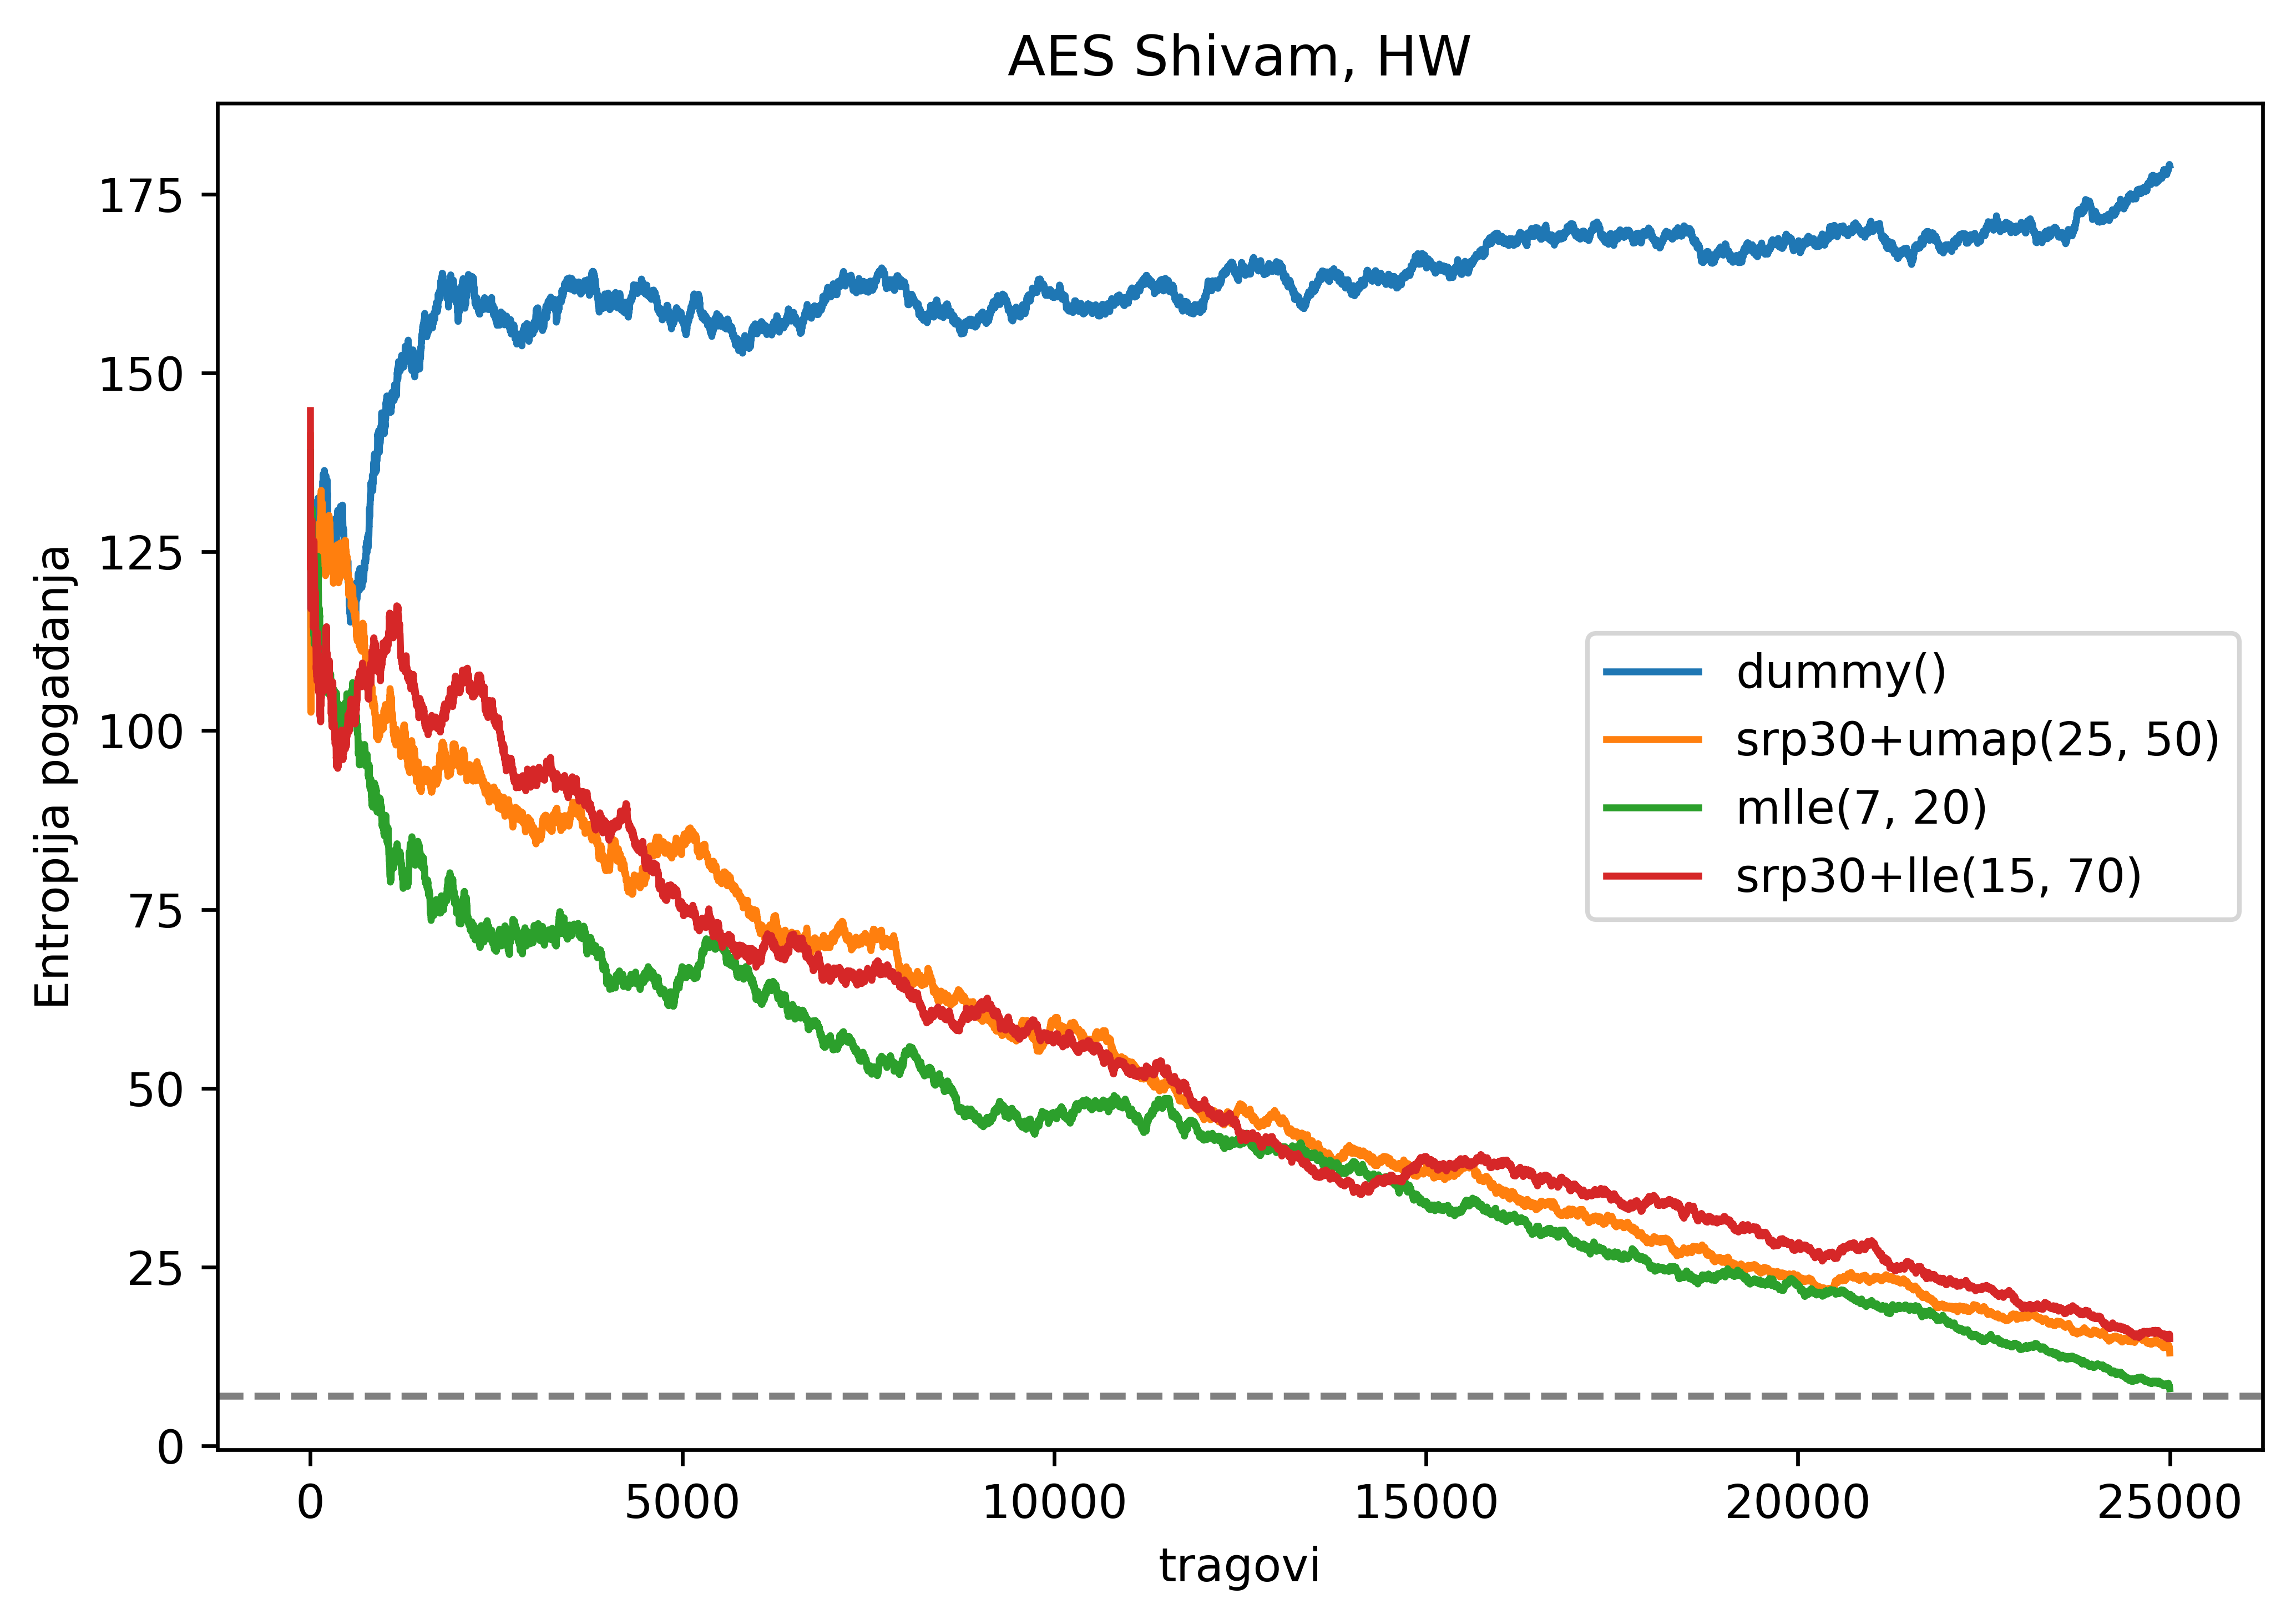
\includegraphics[width=.62\textwidth]{resources/images/application/AES Shivam_HW.png}
        }{%
            \caption{GE za skup AES\_HD - model HW}%
            \label{fig:aes_hw}
        }
        \ttabbox[\FBwidth][]{%
            \resizebox{.32\textwidth}{!}{%
                \setlength\tabcolsep{1.5pt} % default value: 6pt
                \begin{tabular}{lcc|cc}
                    metoda     & $D_m$ & $N_n$ & točnost & $GE_{min}$ \\\hline
                    mlle       & 7     & 20    & 0.23452 & 8          \\
                    srp30+umap & 25    & 50    & 0.05728 & 13         \\
                    srp30+lle  & 15    & 70    & 0.25116 & 15         \\
                    srp30+ltsa & 10    & 70    & 0.22916 & 15.58      \\
                    umap       & 25    & 400   & 0.01376 & 20.56      \\
                    mlle       & 10    & 70    & 0.24068 & 21.96      \\
                    umap       & 10    & 70    & 0.0436  & 22.68      \\
                    srp30+umap & 3     & 10    & 0.22524 & 23.48      \\
                    mlle       & 15    & 150   & 0.24896 & 23.78      \\
                    srp30+ltsa & 15    & 50    & 0.22136 & 23.98      \\
                    dummy      &       &       & 0.24904 & 103        \\
                \end{tabular}
            }
        }{%
            \caption{Rezultati za skup AES\_HD - model HW}%
            \label{tab:aes_hw}
        }
    \end{floatrow}
\end{figure}

\begin{figure}[htb]
    \begin{floatrow}
        \CenterFloatBoxes
        \ffigbox[\FBwidth][]{%
            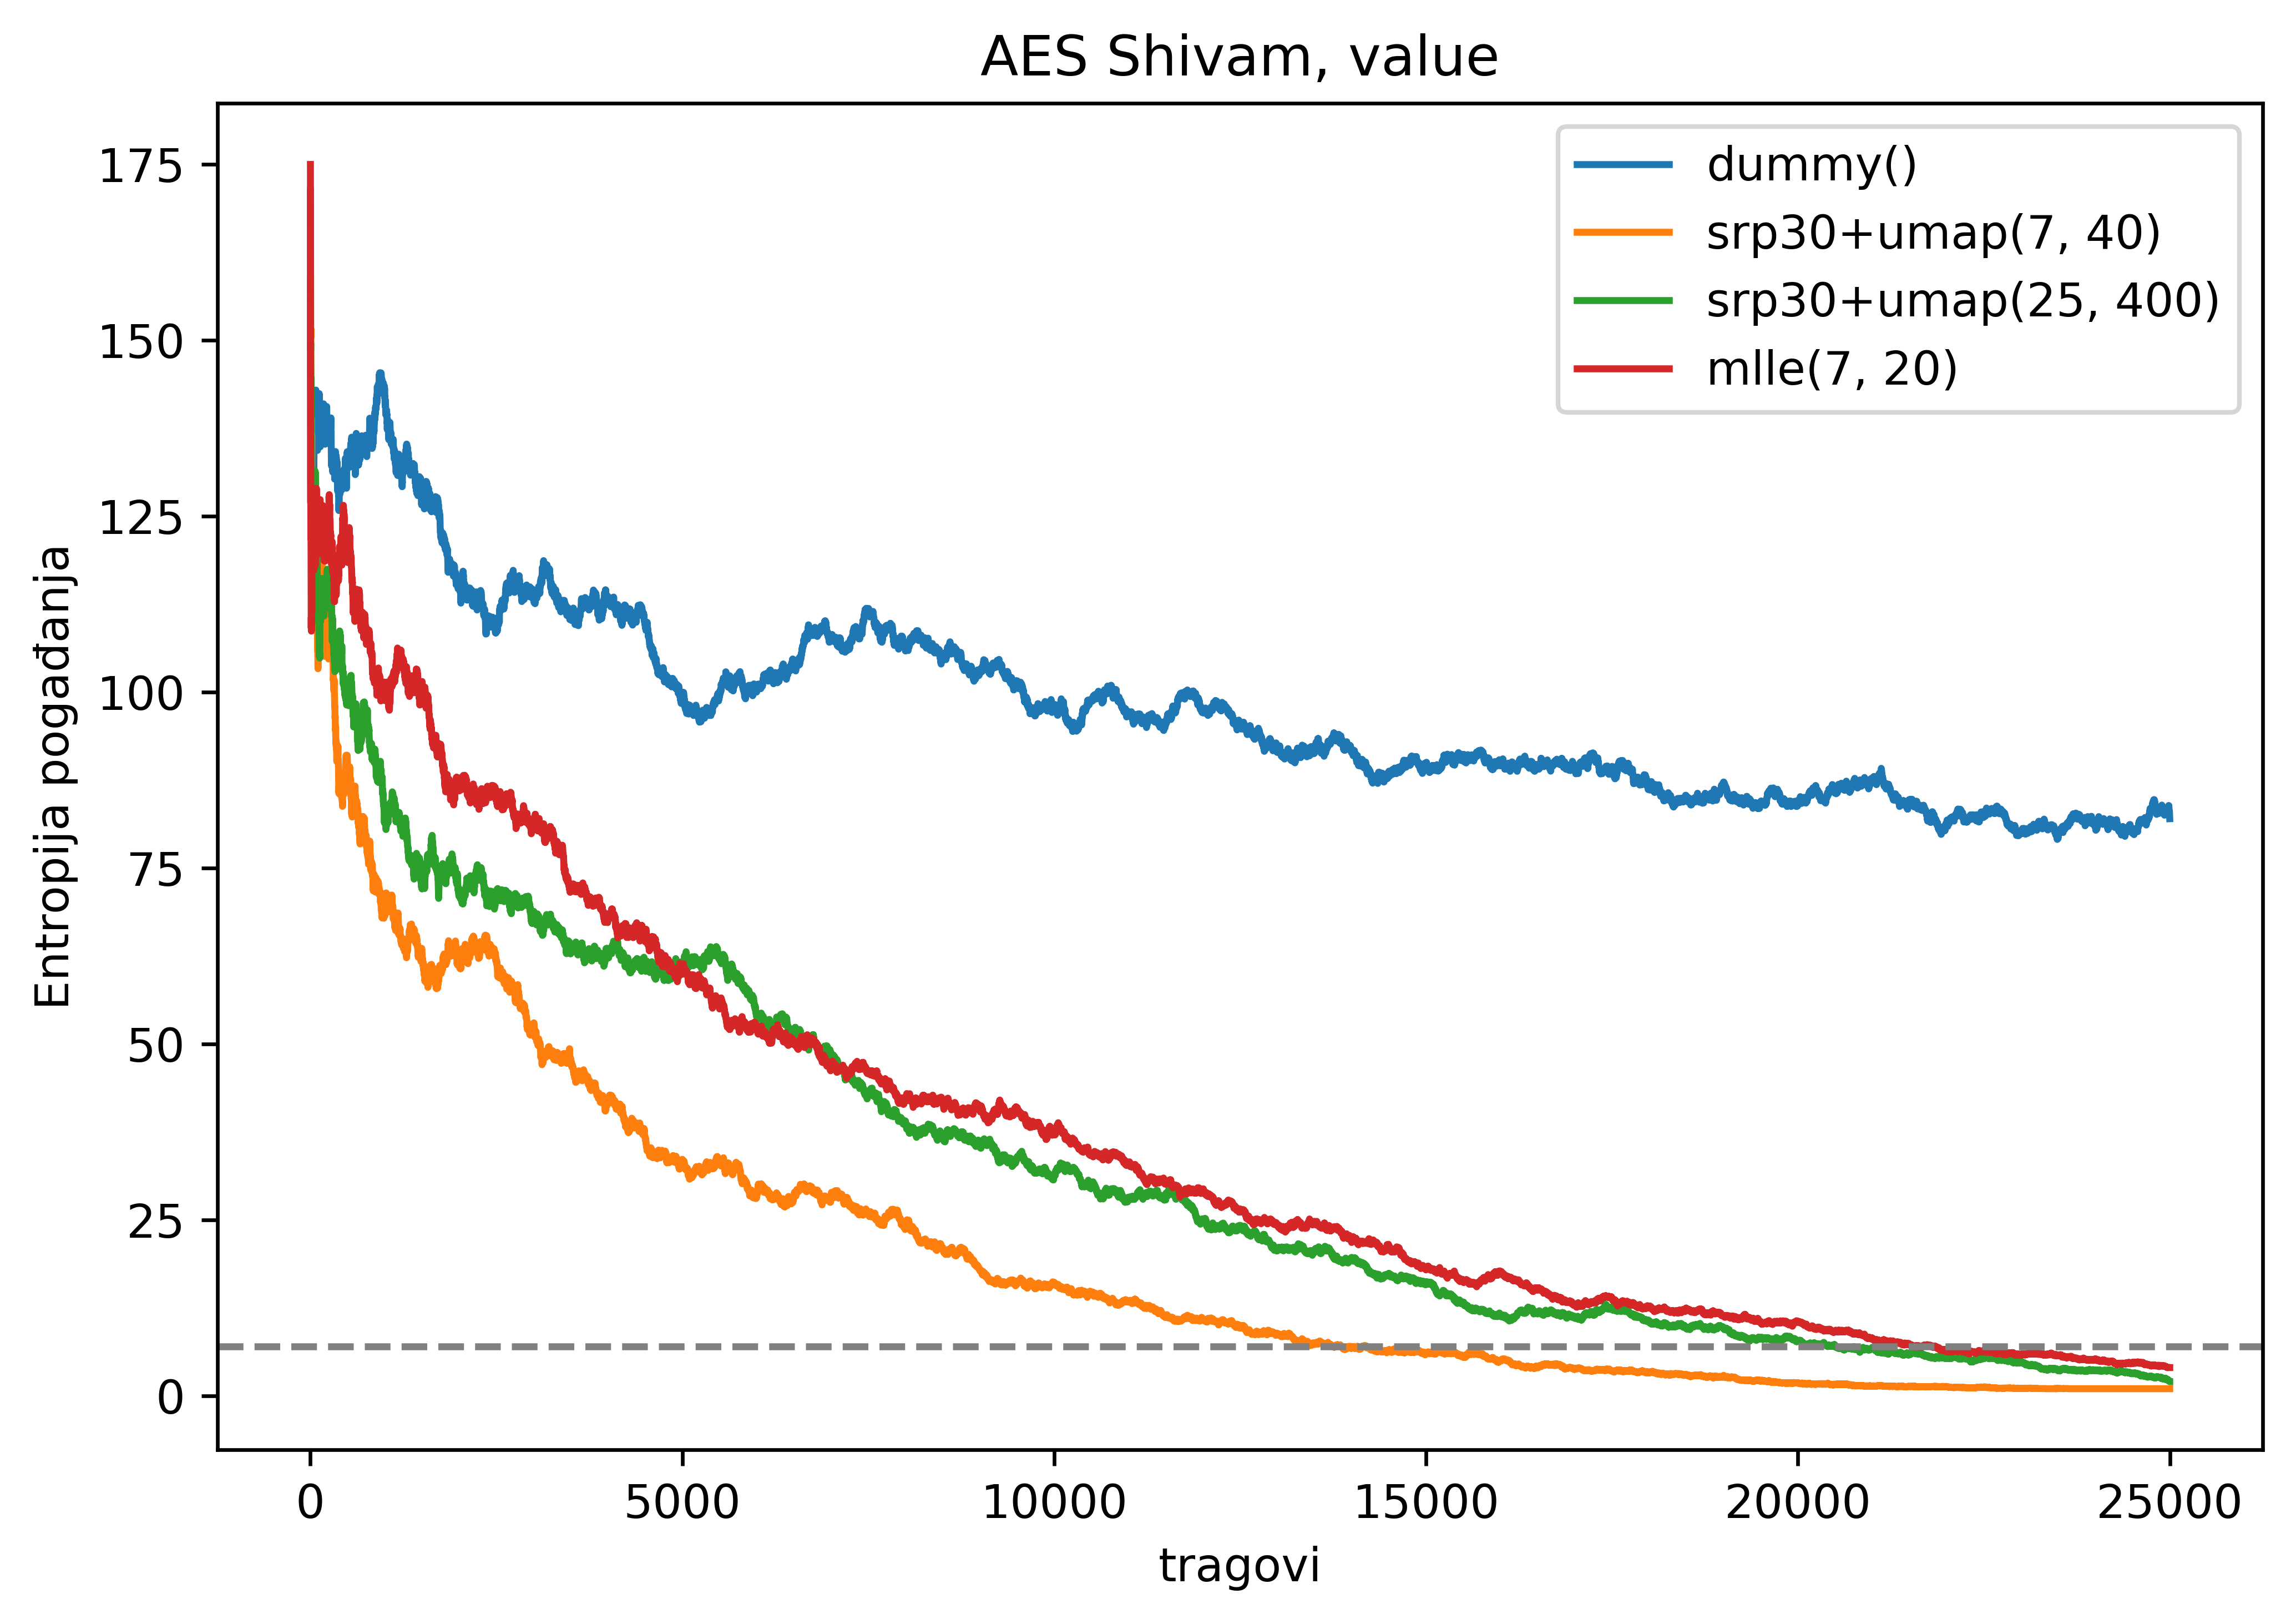
\includegraphics[width=.62\textwidth]{resources/images/application/AES Shivam_value.png}
        }{%
            \caption{GE za skup AES\_HD - value model}%
            \label{fig:aes_value}
        }
        \ttabbox[\FBwidth][]{%
            \resizebox{.32\textwidth}{!}{%
                \setlength\tabcolsep{1.5pt} % default value: 6pt
                \begin{tabular}{lcc|cc}
                    metoda     & $D_m$ & $N_n$ & točnost & $GE_{min}$ \\\hline
                    srp30+umap & 7     & 40    & 0.0038  & 1          \\
                    srp30+umap & 25    & 400   & 0.00364 & 2          \\
                    mlle       & 7     & 20    & 0.00372 & 4          \\
                    srp30+lle  & 10    & 10    & 0.00448 & 6.78       \\
                    srp30+umap & 7     & 20    & 0.00428 & 7          \\
                    pca        & 3     &       & 0.00416 & 7.72       \\
                    mlle       & 20    & 150   & 0.00424 & 7.76       \\
                    srp30+mlle & 15    & 50    & 0.00408 & 8.22       \\
                    srp30+umap & 7     & 10    & 0.004   & 10.96      \\
                    lle        & 7     & 10    & 0.00388 & 11.06      \\
                    dummy      &       &       & 0.00412 & 79.06      \\
                \end{tabular}
            }
        }{%
            \caption{Rezultati za skup AES\_HD - value model}%
            \label{tab:aes_value}
        }
    \end{floatrow}
\end{figure}

\subsection{Random delay}
Konačno, rezultati za posljednji skup podataka, Random delay, koji predstavlja podatke najbliže stvarnosti, dani su u tablicama \ref{tab:rd_hw} i \ref{tab:rd_value} za modele HW i value respektivno. Za model HW rezultati pokazuju da iako nakon mnogo tragova je moguće postići nisku vrijednost GE, korištenje metoda redukcije nije postiglo veliku korist, naspram slučaja di te metode nisu korištene. Ovo je posebno izraženo na slici \ref{fig:rd_hw}. U svakom slučaju, najboljom metodom u ovom slučaju pokazala se metoda srp30 + LLE, s konačnom dimenzijom od 15. Iza nje, kao i u primjeru DPAv4-HW, iskazala se metoda UMAP s malom redukcijom dimenzionalnosti.

No kod korištenja value modela, metodama redukcije dimenzionalnosti postignuti su dobri rezultati izneseni u tablici \ref{tab:rd_value}. Dvije najbolje metode, gotovo ekvivalentnih rezultata, su metoda MLLE s parametrima (10,10) te inačica iste metode s pretprocesiranjem koristeći SRP metodu. Za te metode napad je bio uspješan, tj. postigao nisku GE, nakon samo 2000 tragova. To je vidljivo na slici \ref{fig:rd_value}. Za ovu metodu generalno su najbolje rezultate postigle metode MLLE, HLLE i LTSA, s i bez dodanog koraka metode SRP, dok su metode LLE, PCA i UMAP pokazale lošije rezultate. 

\begin{figure}[htb]
    \begin{floatrow}
        \CenterFloatBoxes
        \ffigbox[\FBwidth][]{%
            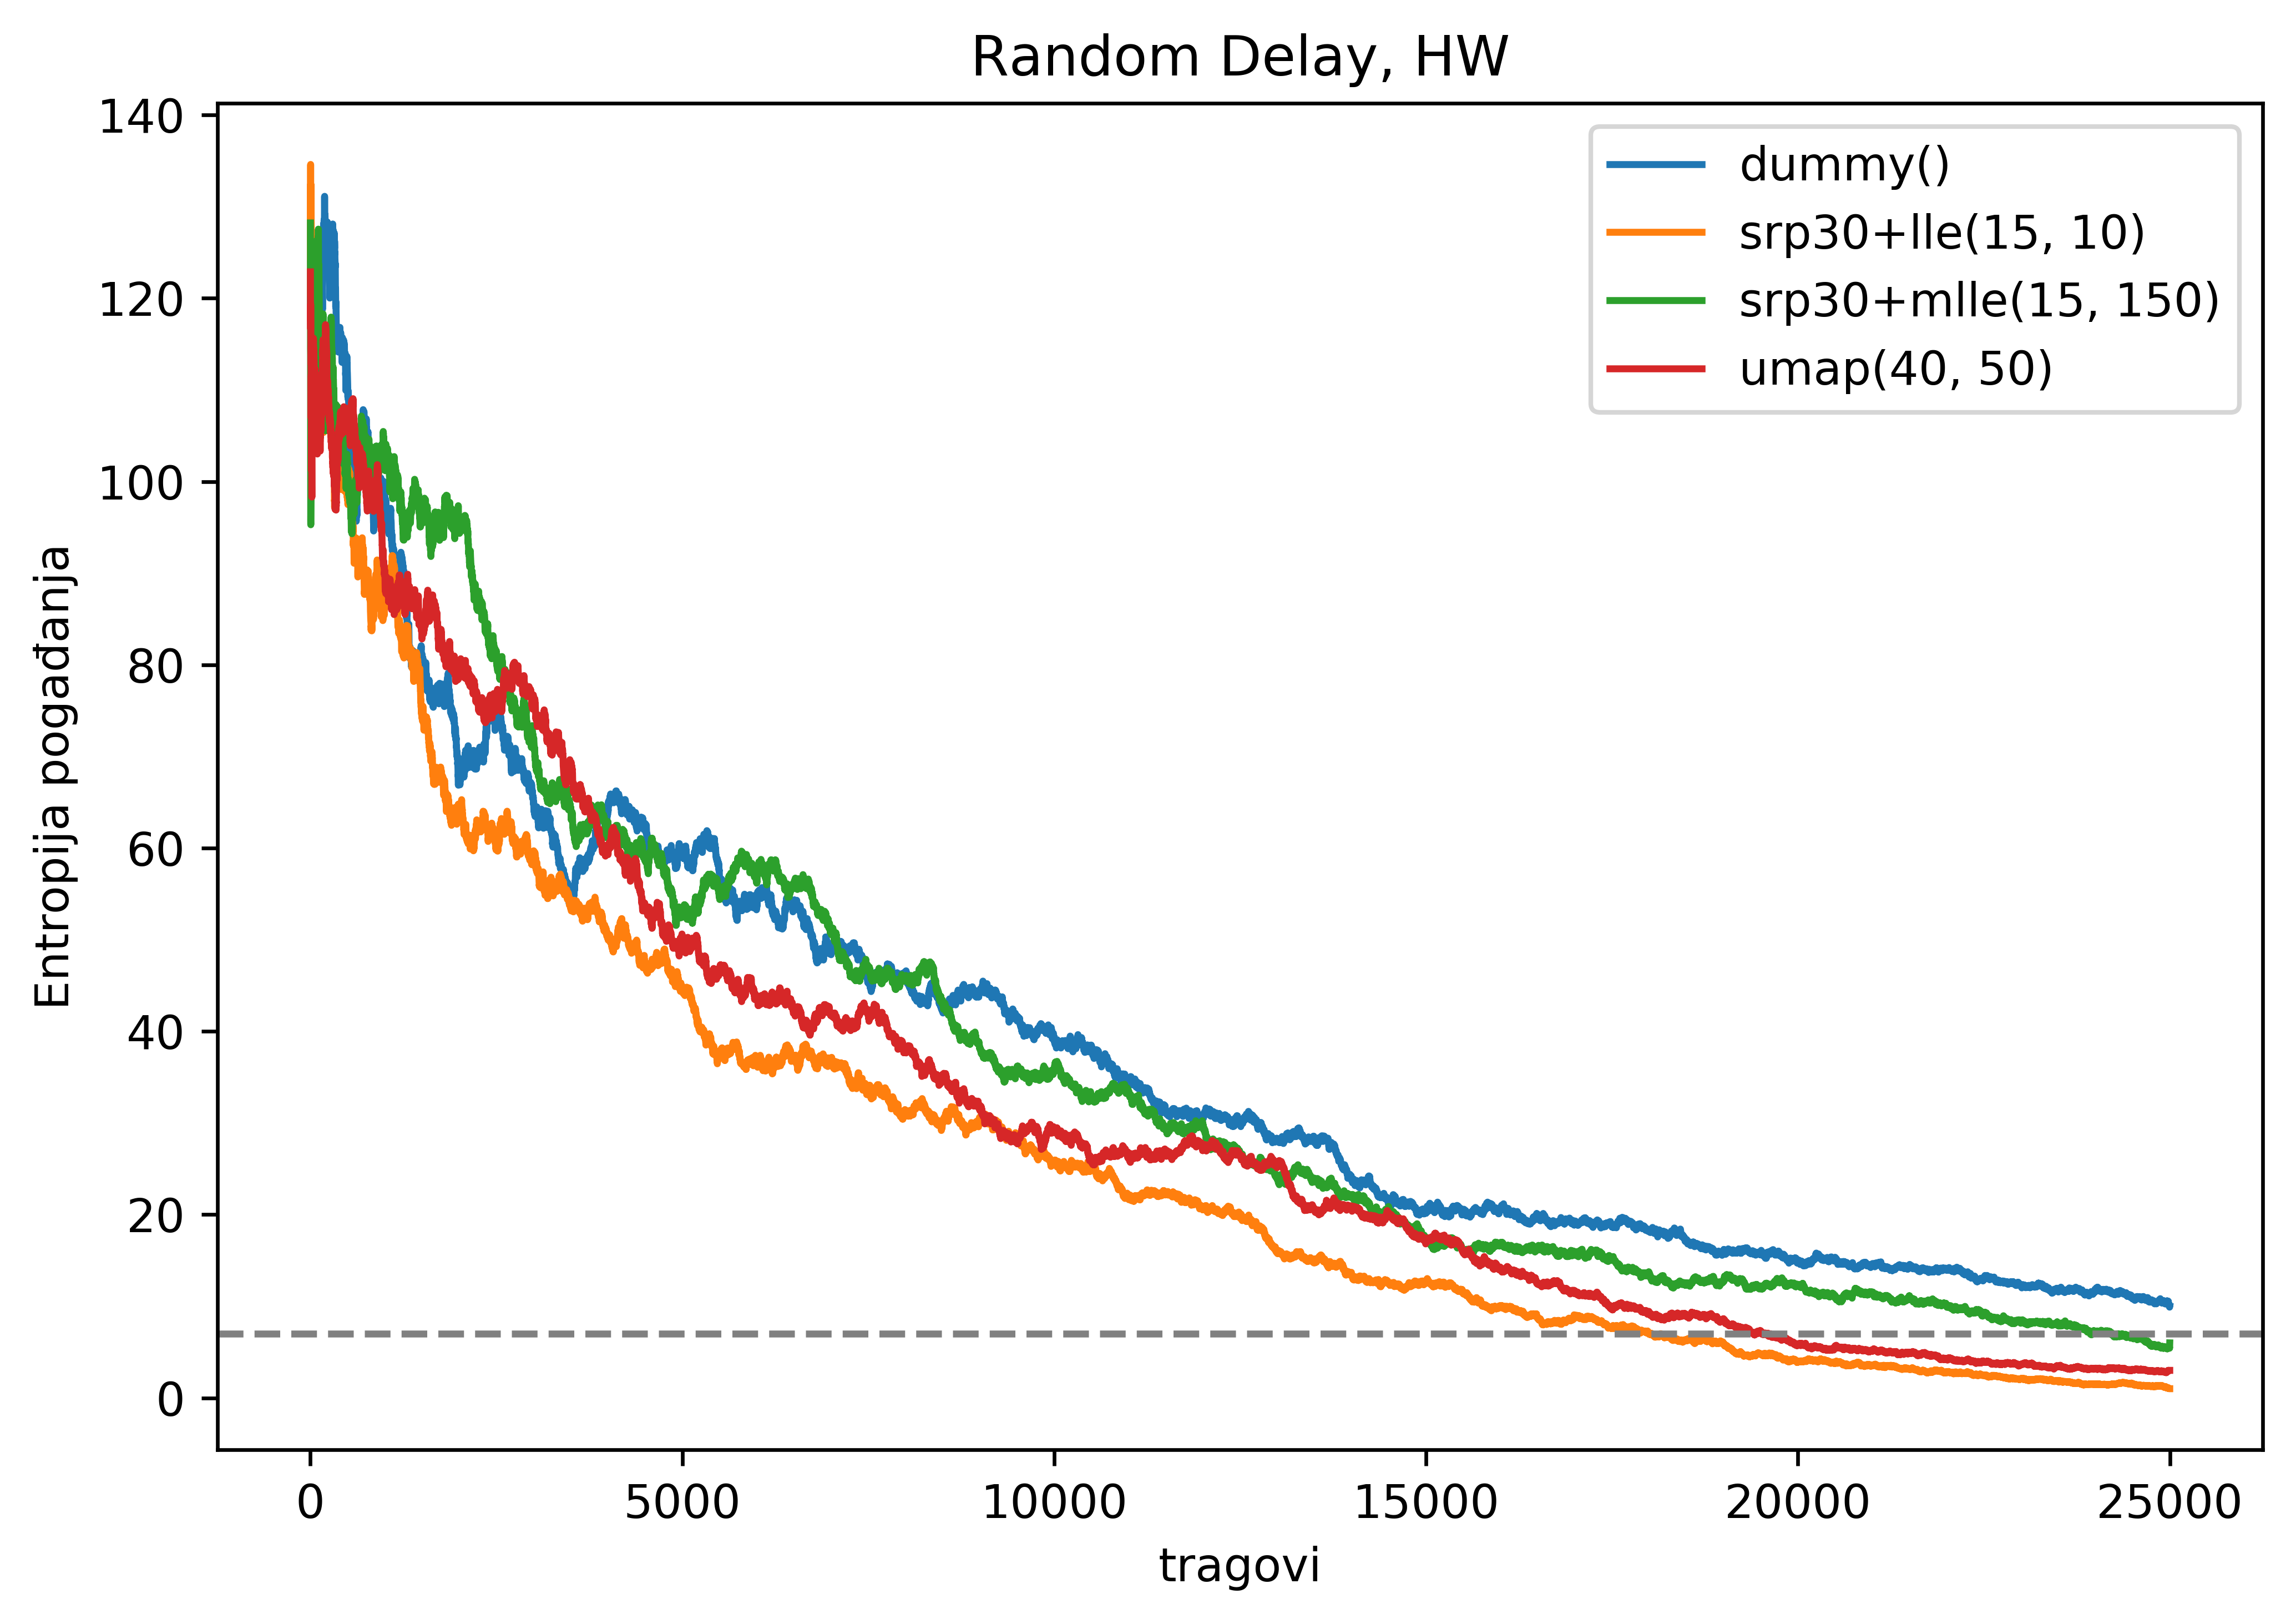
\includegraphics[width=.62\textwidth]{resources/images/application/Random Delay_HW.png}
        }{%
            \caption{GE za skup Random Delay - model HW}%
            \label{fig:rd_hw}
        }
        \ttabbox[\FBwidth][]{%
            \resizebox{.32\textwidth}{!}{%
                \setlength\tabcolsep{1.5pt} % default value: 6pt
                \begin{tabular}{lcc|cc}
                    metoda     & $D_m$ & $N_n$ & točnost & $GE_{min}$ \\\hline
                    srp30+lle  & 15    & 10    & 0.24632 & 1          \\
                    umap       & 40    & 50    & 0.03268 & 2.74       \\
                    srp30+mlle & 15    & 150   & 0.252   & 5.34       \\
                    srp30+lle  & 10    & 70    & 0.24924 & 5.38       \\
                    ltsa       & 10    & 10    & 0.24428 & 6.8        \\
                    mlle       & 7     & 10    & 0.2378  & 7          \\
                    umap       & 7     & 40    & 0.04592 & 8.82       \\
                    srp30+hlle & 25    & 400   & 0.25472 & 9.74       \\
                    dummy      &       &       & 0.25728 & 9.9        \\
                    srp30+lle  & 3     & 10    & 0.2288  & 10.06      \\
                    srp30+lle  & 7     & 40    & 0.24364 & 10.16      \\
                \end{tabular}
            }
        }{%
            \caption{Rezultati za skup Random Delay - model HW}%
            \label{tab:rd_hw}
        }
    \end{floatrow}
\end{figure}

\begin{figure}[htb]
    \begin{floatrow}
        \CenterFloatBoxes
        \ffigbox[\FBwidth][]{%
            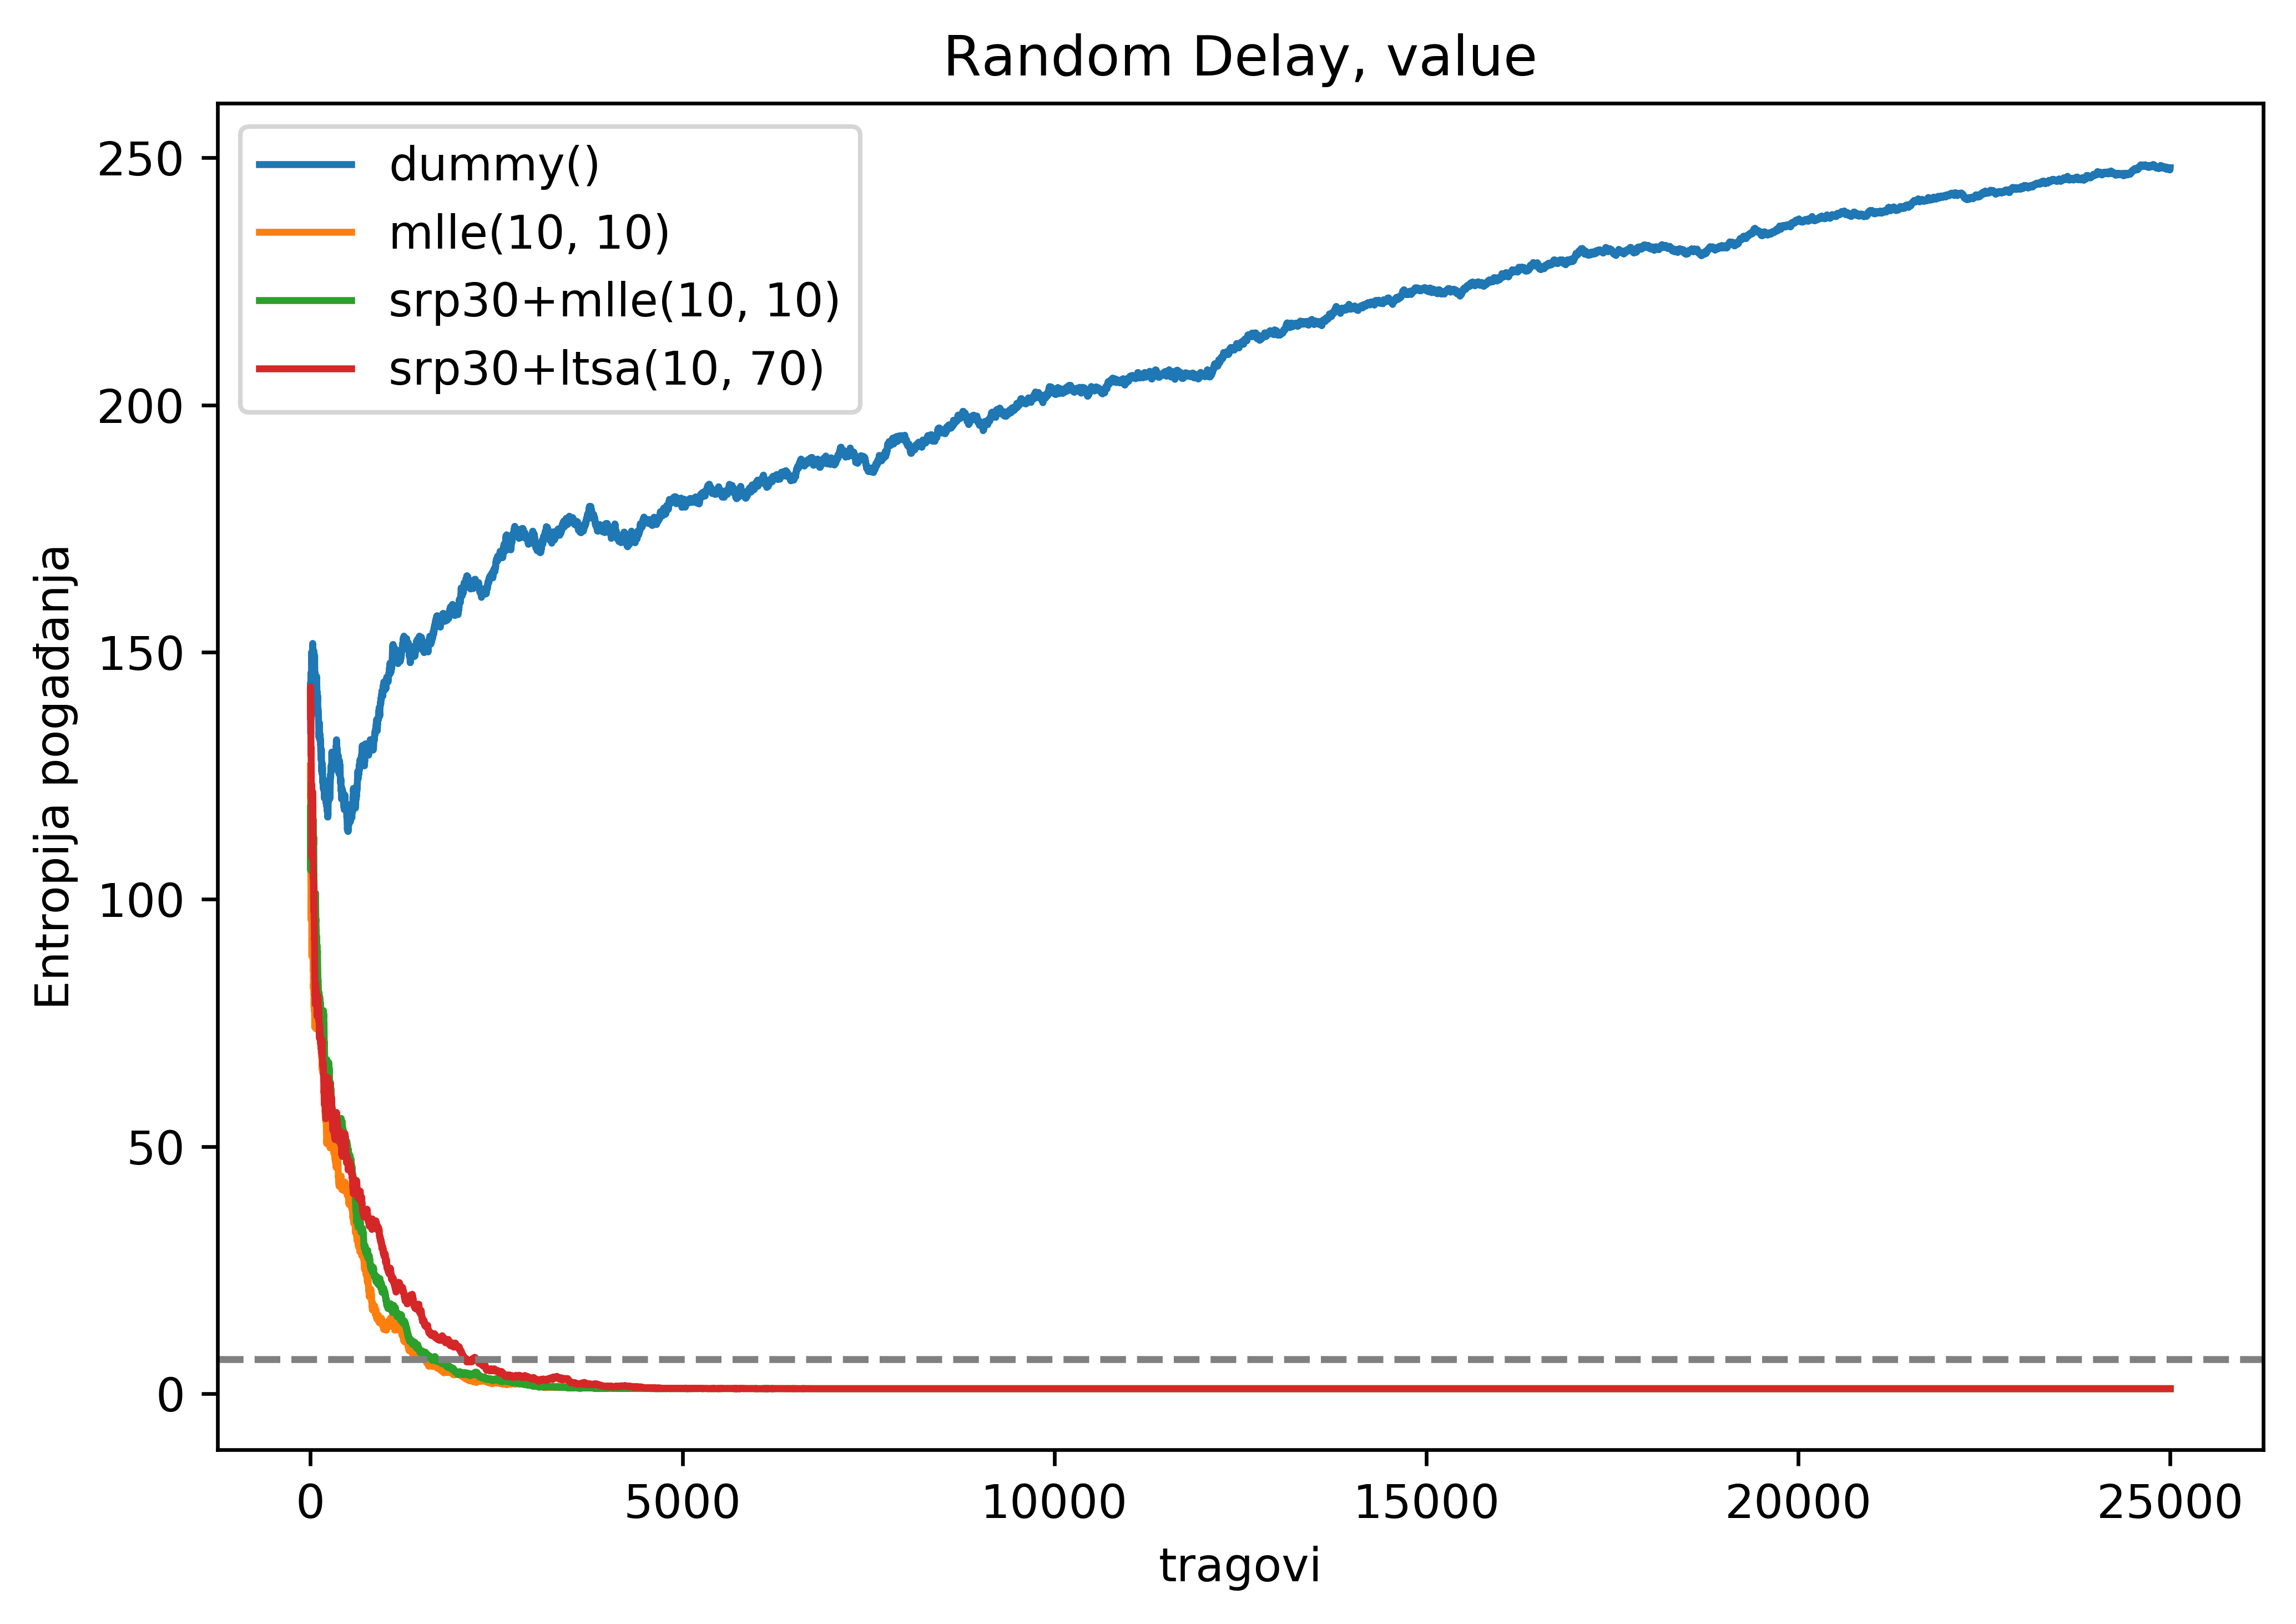
\includegraphics[width=.62\textwidth]{resources/images/application/Random Delay_value.png}
        }{%
            \caption{GE za skup Random Delay - value model}%
            \label{fig:rd_value}
        }
        \ttabbox[\FBwidth][]{%
            \resizebox{.32\textwidth}{!}{%
                \setlength\tabcolsep{1.5pt} % default value: 6pt
                \begin{tabular}{lcc|cc}
                    metoda     & $D_m$ & $N_n$ & točnost & $GE_{min}$ \\\hline
                    srp30+mlle & 10    & 10    & 0.00428 & 1          \\
                    mlle       & 10    & 10    & 0.00428 & 1          \\
                    srp30+ltsa & 10    & 70    & 0.00432 & 1          \\
                    ltsa       & 15    & 70    & 0.00432 & 1          \\
                    srp30+ltsa & 25    & 50    & 0.00424 & 1          \\
                    srp30+hlle & 10    & 70    & 0.00428 & 1          \\
                    ltsa       & 25    & 50    & 0.00428 & 1          \\
                    ltsa       & 40    & 50    & 0.00424 & 1          \\
                    srp30+ltsa & 15    & 50    & 0.00424 & 1          \\
                    ltsa       & 10    & 70    & 0.00432 & 1          \\
                    dummy      &       &       & 0.00408 & 113.74     \\
                \end{tabular}
            }
        }{%
            \caption{Rezultati za skup Random Delay - value model}%
            \label{tab:rd_value}

        }
    \end{floatrow}
\end{figure}

\section{Diskusija}
U prošlom odjeljku težina je bila na specifičnim skupovima podataka, dok u ovom odjeljku cilj je iznijeti generalnije zaključke. Ono što je proizašlo iz rezultata je da promjena parametara i metoda korištenih drastično utječe na rezultat. Ovo odgovara poznatom teoremu o nepostojanju besplatnog ručka \engl{"No Free Lunch" theorem} koji kaže da ne postoji jedan algoritam koji ispunjava potrebe svih problema. 

Također, pokazalo se kako smanjivanje dimenzije metodom rijetkih slučajnih projekcija prije nego što se izvodi učenje mnogostrukosti, osim što smanjuje trajanje izvođenja algoritma, dodatno i povećava performanse u kontekstu analize koja koristi sporedna sredstva. Postoji manjak empirijskih istraživanja na ovu temu, te ona definitivno prezentira razne mogućnosti. 

Za korištene skupove podataka pokazalo se kako iako HW model ima značajno veću točnost, koristeći mjeru entropije pogađanja, u ovom kontekstu boljim se modelom pokazao value model. Kod HW modela je za očekivati veća točnost klasifikacije jer je jednostavnije napraviti klasifikaciju u 9 razreda nego u 256 razreda. Što se tiče boljih ukupnih performansi na value modelu, jedno moguće objašnjenje je da ako na kreaciju sporednih sredstava gledamo kao neku transformaciju originalnih podataka $P$ u sporedna sredstva $S$, $\Phi: P \mapsto S$, na učenje mnogostrukosti možemo gledati kao traženje inverzne transformacije $\Phi^{-1}: S \mapsto P$. Ovaj zadatak je lakši kada imamo direktne vrijednosti dobivene mjerenjem nego kada je uvedena dodatna razina, u ovom slučaju Hammingova težina. 
Bolju efikasnost napada moguće je postići optimizacijom hiperparametara klasifikatora ili korištenjem dodatnih klasifikatora.

\chapter{Zaključak}
U ovom diplomskom radu razmatrala se primjena postupaka učenja mnogostrukosti za povećavanje učinkovitosti analize koja koristi sporedna sredstva kriptografskih uređaja (SCA) te su detaljno opisana oba polja analize sporednih sredstava i redukcije dimenzionalnosti. Za SCA dan je uvid u granu, opisane su osnove sporednih sredstava i napravljena je taksonomska podjela ove grane. Nakon toga su opisani razni napadi te širina njihove primjene. Zatim su opisane i razne implementirane protumjere protiv SCA napada. Uz SCA proučena je i ideja redukcije dimenzionalnosti koja je u ovom radu podijeljena na dvije velike pod skupine, a to su linearna redukcija dimenzionalnosti i učenje mnogostrukosti (nelinearna redukcija dimenzionalnosti). Naglasak u ovom radu je na metode učenja mnogostrukosti te je iz skupine linearne redukcije kao jedna od referentnih metoda uzeta i vrlo popularna metoda PCA. Osim PCA, dodatna referentna vrijednost u ovom radu je kako se izvedeni eksperimenti ponašaju kada nije implementirana nikakva redukcija dimenzionalnosti. Uz ovo korištena je dodatno hibridna metoda redukcije dimenzionalnosti koja prije metoda učenja mnogostrukosti izvršava jednostavniju metodu rijetkih slučajnih projekcija kako bi se napravila redukcija u međuprostor na kojem se onda provode opisane metode. Iz dobivenih rezultata vidljivo je da su korištene metode vrlo osjetljive na promjenu hiperparametara te je njihova optimizacija ključna za postizanje dobrih rezultata. Također, generalno se pokazalo kako je bolje koristiti model koji uzima međuvrijednosti u ovom kontekstu, nego model s Hammingovom težinom, koji se češće smatra boljim. Prezentirana hibridna metoda pokazala se kao izvrstan način za ne samo skraćivanje vremena izvođenja, već i za postizanje boljih rezultata. Dodatne kombinacije jednostavnijih i složenijih metoda su moguće koje imaju potencijal rezultirati i boljim performansama. Primjerice umjesto rijetkih slučajnih projekcija u istu se svrhu mogu koristiti i gaussianske slučajne projekcije. Korištenje ovakvih metoda moglo bi rezultirati još boljim rezultatima na više dimenzionalnim skupovima i na njima uvesti velike doprinose u kontekstu efikasnosti algoritma za redukciju dimenzionalnosti. Također bolji rezultati napada mogu se postići odabirom specifičnog klasifikatora i njegovih parametara za željenu metodu redukcije dimenzionalnosti. Ovo nije bilo u okviru ovog radate je cilj bio usporediti razne tehnike učenja mnogostrukosti u kontekstu SCA. Usprkos tome na svim skupovima uspješno je postignuta dovoljno niska entropija pogađanja koristeći relativno mali skup značajki veličine 50. Na skupu podataka koji implementira slučajno kašnjenje kao protumjeru postignuti su odlični rezultati te je dovoljno niska vrijednost entropije pogađanja postignuta nakon prosječno 2000 tragova.


\bibliography{literatura}
\bibliographystyle{fer}

\begin{sazetak}
    Cilj ovog diplomskog rada je razmotriti primjenu postupaka učenja mnogostrukosti kako bi se povećala učinkovitost analize koja koristi sporedna sredstva kriptografskih uređaja (SCA). U sklopu toga detaljno su opisana oba polja SCA i redukcije dimenzionalnosti te za njih ponaosob metode korištene u tom polju. Iako je naglasak u ovom radu na metode učenja mnogostrukosti, kao jedna od referentnih metoda uzeta je i vrlo popularna metoda PCA. Dodatno je korištena hibridna metoda redukcije dimenzionalnosti koja prije metoda učenja mnogostrukosti izvodi metodu rijetkih slučajnih projekcija kako bi se napravila redukcija u međuprostor. Za konačnu klasifikaciju koristi se metoda slučajnih šuma zbog velike otpornosti na smetnje.

    \kljucnerijeci{učenje mnogostrukosti, analiza koja koristi sporedna svojstva (SCA), entropija pogađanja (GE), redukcija dimenzionalnosti, AES}
\end{sazetak}

\begin{abstract}
    This thesis aims to study the application of manifold learning techniques with the intent of increasing the efficiency of side-channel analysis (SCA). With this in mind,  both SCA, dimensionality reduction fields, and their respected practices are described. Even though the emphasis in this paper is on manifold learning, as one of the reference methods, highly popular PCA method was adopted. Additionally, a hybrid dimensionality reduction method was applied, in which, before the manifold learning method, sparse random projections are performed to reduce data into interspace. The random forest method is used for the final classification due to its high resistance to noise.

    \keywords{manifold learning, side-channel analysis (SCA), guessing entropy (GE), dimensionality reduction, AES}
\end{abstract}

\end{document}